\documentclass{beamer}

\usetheme[progressbar=frametitle, block=fill]{metropolis}
% \usepackage{fontspec}
\usepackage{appendixnumberbeamer}
\usepackage{booktabs}
\usepackage{multirow}
\usepackage{amsmath}
\usepackage{amssymb}
\usepackage{listings}
\usepackage{tikz}
\usepackage{pgf}
\usetikzlibrary{arrows.meta, shapes, positioning, calc, fit, backgrounds}
\usepackage{xcolor}
\usepackage{arydshln}

% ---- Lean listings ----
\definecolor{keywordcolor}{rgb}{0.7, 0.1, 0.1}
\definecolor{tacticcolor}{rgb}{0.0, 0.1, 0.6}
\definecolor{commentcolor}{rgb}{0.4, 0.4, 0.4}
\definecolor{symbolcolor}{rgb}{0.0, 0.1, 0.6}
\definecolor{sortcolor}{rgb}{0.1, 0.5, 0.1}
\definecolor{attributecolor}{rgb}{0.7, 0.1, 0.1}
\def\lstlanguagefiles{lstlean.sty}
\lstset{language=lean, basicstyle=\footnotesize\ttfamily}

% ---- Accent colors ----
\definecolor{improverBlue}{HTML}{2C6EAB}
\definecolor{improverGreen}{HTML}{14B03D}
\definecolor{improverOrange}{HTML}{EB811B}
\definecolor{improverRed}{HTML}{C0392B}
\definecolor{accentTeal}{HTML}{16A085}

\newcommand{\highlight}[1]{\textcolor{improverOrange}{\textbf{#1}}}
\newcommand{\methodname}{ImProver}
\newcommand{\good}[1]{\textcolor{improverGreen}{\textbf{#1}}}
\newcommand{\bad}[1]{\textcolor{improverRed}{\textbf{#1}}}

\graphicspath{{./figures/}}

\title{Neural Proof Optimization}
\author{Riyaz Ahuja}
\institute{Department of Mathematics, Carnegie Mellon University}
\date{April 20, 2026}

% ================================================================
\begin{document}
% ================================================================

\maketitle

\begin{frame}{Outline}
\tableofcontents
\end{frame}

\begin{frame}{Core Contributions}
\vspace{0.3em}
\begin{enumerate}\setlength{\itemsep}{10pt}
  \item[\textbf{C1.}] \textbf{Task formalization}\\
    \small Proof optimization defined over a verified proof $(c,x,y_0)$ and arbitrary metric $\mu$; NTP shown to be a strict special case
  \item[\textbf{C2.}] \textbf{ImProver: agentic proof optimizer} \hfill{\small\textit{ICLR 2025}}\\
    \small GPT-4o agent with CoS prompting, iterative refinement, and RAG; outperforms naive GPT-4o by $423$--$778\%$ on undergraduate proofs
  \item[\textbf{C3.}] \textbf{ImProver~2: trained small model} \hfill{\small\textit{ICML 2026 submitted}}\\
    \small 7B model trained via IRPO self-improvement + neurosymbolic scaffold; outperforms 671B models on structural metrics at a fraction of the cost
  \item[\textbf{C4.}] \textbf{Specialization beats scale}\\
    \small Gains track formal-structure exposure (CoS, neurosymbolic augmentation), not model size; proof optimization is a specialization problem
\end{enumerate}
\end{frame}

% ================================================================
\section{Motivation}
% ================================================================

\begin{frame}{Mathematical Collaboration and the PNT}

% In 1896, Jacques Hadamard and Charles Jean de la Vallée Poussin independently proved one of the central results of nineteenth-century mathematics: the number of primes less than $n$ grows asymptotically as $n/\ln n$. The Prime Number Theorem had been conjectured by Gauss and Legendre nearly a century earlier from numerical evidence, but its proof required mathematical tools entirely foreign at the time. Indeed, it took Riemann's study of the deep connection between the distribution of primes and the zeros of the zeta function --- combined with subsequent advances in contour integration, the theory of entire functions, and analytic continuation --- that ultimately made the proof possible. The PNT was not proved by a direct combinatorial or number theoretic attack on the primes, rather, it took centuries of collaborative development of shared infrastructure and techniques across disparate domains of mathematics before the pieces could be put together.


\begin{figure}
    \centering
    % \includegraphics[width=\textwidth]{figures/flt_dependency_graph_placeholder.pdf}
    % 
\includegraphics[scale=0.075]{figures/slides/PNT_dependency.png}
    % \caption{Schematic dependency graph for the Lean formalization effort around the Prime Number Theorem (center). Radial distance measures dependency depth and angular distance measures domain similarity as computed by namespace distance.}
    \label{fig:pnt-dependency-graph}
\end{figure}


\end{frame}


\begin{frame}{Mathematical Collaboration and the PNT}


\begin{columns}[T]
\begin{column}{0.50\textwidth}
\begin{figure}
% 
\includegraphics[width=\linewidth]{figures/slides/PNT_dependency.png}
\end{figure}
\end{column}
\begin{column}{0.46\textwidth}
\vspace{1em}
% In 1896, Jacques Hadamard and Charles Jean de la Vallée Poussin independently proved one of the central results of nineteenth-century mathematics: the number of primes less than $n$ grows asymptotically as $n/\ln n$. The Prime Number Theorem had been conjectured by Gauss and Legendre nearly a century earlier from numerical evidence, but its proof required mathematical tools entirely foreign at the time. Indeed, it took Riemann's study of the deep connection between the distribution of primes and the zeros of the zeta function --- combined with subsequent advances in contour integration, the theory of entire functions, and analytic continuation --- that ultimately made the proof possible. The PNT was not proved by a direct combinatorial or number theoretic attack on the primes, rather, it took centuries of collaborative development of shared infrastructure and techniques across disparate domains of mathematics before the pieces could be put together.
\begin{theorem}
    The number of primes less than $n$ grows as $O(n / \ln n)$
\end{theorem}
\begin{itemize}
    \item Proven independently by Hadamard and Poussin in 1896
    \item However, conjectured nearly 100 years prior (Gauss, Legendre)
    \item What was the gap?
\end{itemize}


% Within DeepSeek family: larger models score higher --- scale helps.\\[0.8em]
% But \textbf{ImProver~2 at 7B} beats DeepSeek at \textbf{671B} on all three metrics.\\[0.8em]
% \begin{alertblock}{}
%   \small Proof optimization is a \textbf{specialization} problem, not just a scale problem.
% \end{alertblock}
\end{column}
\end{columns}

\end{frame}


\begin{frame}{Mathematical Collaboration and the PNT}


\begin{columns}[T]
\begin{column}{0.50\textwidth}
\begin{figure}
% 
\includegraphics[width=\linewidth]{figures/slides/PNT_dependency.png}
\end{figure}
\end{column}
\begin{column}{0.46\textwidth}
\vspace{1em}
% In 1896, Jacques Hadamard and Charles Jean de la Vallée Poussin independently proved one of the central results of nineteenth-century mathematics: the number of primes less than $n$ grows asymptotically as $n/\ln n$. The Prime Number Theorem had been conjectured by Gauss and Legendre nearly a century earlier from numerical evidence, but its proof required mathematical tools entirely foreign at the time. Indeed, it took Riemann's study of the deep connection between the distribution of primes and the zeros of the zeta function --- combined with subsequent advances in contour integration, the theory of entire functions, and analytic continuation --- that ultimately made the proof possible. The PNT was not proved by a direct combinatorial or number theoretic attack on the primes, rather, it took centuries of collaborative development of shared infrastructure and techniques across disparate domains of mathematics before the pieces could be put together.
\textbf{Infrastructure:}
\begin{itemize}
    \item Hadamard, Poussin both employed complex analytic techniques.
    \item Without 100 years of development of the shared infrastructure on the zeta function, contour integration, analytic continuation, etc., the proof would have been impossible.
\end{itemize}

\end{column}
\end{columns}

\end{frame}




\begin{frame}{Proof Assistants}

Despite the importance of shared public infrastructure and library development in mathematics, traditional collaboration is fundamentally limited by a \textit{trust bottleneck}.

% \includegraphics[width=\linewidth]{figures/slides/plot1_arxiv_authors.png}


\end{frame}

\begin{frame}{Proof Assistants}

However, proof assistants allow for the decentralization of trust: anyone, anywhere can contribute as their correctness is formally checked and verified. This allows for larger scale collaboration.

% \includegraphics[width=\linewidth]{figures/slides/plot2_comparison.png}

\end{frame}




\begin{frame}[fragile]{Proof Assistants}

Lean 4 is one such proof assistant, with an especially large and robust infrastructure library.


% \begin{columns}[T]
% \begin{column}{0.50\textwidth}
% \begin{figure}

\begin{itemize}
  \item Proofs are programs: Lean's type system enforces logical correctness
  \item Each tactic transforms the proof state: the current hypotheses and goals
  \item A small, trusted kernel checks every step
\end{itemize}

% \end{figure}
% \end{column}
% \begin{column}{0.46\textwidth}
\vspace{1em}
\begin{lstlisting}
-- set intersection distributes over union
example : s $\cap$ (t $\cup$ u) =
          (s $\cap$ t) $\cup$ (s $\cap$ u) := by
  ext x
  simp only [Set.mem_inter_iff,
             Set.mem_union]
  tauto
\end{lstlisting}
% \end{column}
% \end{columns}


% \includegraphics[width=\linewidth]{figures/slides/lines_mathlib.png}



\end{frame}

\begin{frame}{Proof Assistants Enable Decentralized Trust}
\vspace{0.8em}
\begin{itemize}\setlength{\itemsep}{10pt}
  \item Lean 4: a proof assistant where proofs are checked by a small, audited \textbf{kernel}
  \item You trust the kernel, not the author
  \item Anyone, anywhere can contribute --- correctness is checked mechanically
  \item This enables \highlight{trust-free, decentralized formal mathematics at scale}
\end{itemize}
\vspace{0.8em}
\begin{exampleblock}{}
  \centering A formal proof is a machine-checkable certificate, not a social agreement.
\end{exampleblock}
\end{frame}

\begin{frame}[fragile]{What a Lean Proof Looks Like}
\vspace{0.5em}
\begin{itemize}\setlength{\itemsep}{6pt}
  \item Proofs are programs: Lean's type system enforces logical correctness
  \item Each \emph{tactic} transforms the proof state: the current hypotheses and goals
  \item The kernel checks every step
\end{itemize}
\vspace{0.6em}
\begin{lstlisting}[basicstyle=\footnotesize\ttfamily]
-- set intersection distributes over union
example : s $\cap$ (t $\cup$ u) =
          (s $\cap$ t) $\cup$ (s $\cap$ u) := by
  ext x
  simp only [Set.mem_inter_iff,
             Set.mem_union]
  tauto
\end{lstlisting}
\end{frame}

\begin{frame}{Mathlib: Formal Mathematics at Scale}
\vspace{0.8em}
\begin{itemize}\setlength{\itemsep}{10pt}
  \item Lean's community mathematics library
  \item $>100{,}000$ formal lemmas: algebra, topology, analysis, number theory, and more
  \item Hundreds of active contributors worldwide
  \item \highlight{Growing by thousands of lemmas per month}
\end{itemize}
\vspace{0.8em}
\begin{exampleblock}{}
  \centering Lean's trust-free model makes this scale possible.
\end{exampleblock}
\end{frame}

\begin{frame}{Mathlib is Growing Exponentially}
\begin{center}
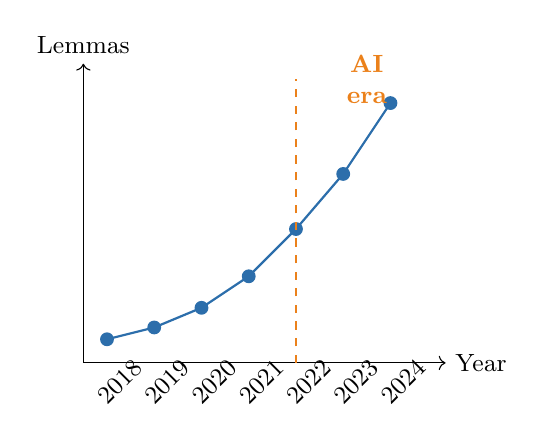
\begin{tikzpicture}[font=\normalsize, scale=1.0]
\draw[->] (0,0) -- (0,3.8) node[above] {\small Lemmas};
\draw[->] (0,0) -- (4.6,0) node[right] {\small Year};
\foreach \x/\y/\lbl in {
  0.3/0.3/2018, 0.9/0.45/2019, 1.5/0.7/2020,
  2.1/1.1/2021, 2.7/1.7/2022, 3.3/2.4/2023, 3.9/3.3/2024}
{
  \fill[improverBlue] (\x,\y) circle (2.5pt);
  \node[below, font=\small, rotate=45] at (\x, -0.08) {\lbl};
}
\draw[improverBlue, thick]
  (0.3,0.3)--(0.9,0.45)--(1.5,0.7)--(2.1,1.1)--(2.7,1.7)--(3.3,2.4)--(3.9,3.3);
\draw[improverOrange, dashed, thick] (2.7,0) -- (2.7,3.6);
\node[improverOrange, font=\small\bfseries, align=center] at (3.6,3.6) {AI\\era};
\end{tikzpicture}
\end{center}
\vspace{0.3em}
\small Growth already outpaces what human reviewers can reliably curate.
\end{frame}

\begin{frame}{But: Review is Still Manual}
\vspace{0.8em}
\begin{itemize}\setlength{\itemsep}{10pt}
  \item Every Mathlib PR is reviewed by human maintainers
  \item Reviewers check: mathematical correctness, style, documentation, robustness
  \item Contributions must be rewritten until they meet the library's style guidelines
  \item As the library grows, inter-dependencies make reviews harder
\end{itemize}
\vspace{0.8em}
\begin{alertblock}{}
  \centering Even today, the growth rate already stresses human capacity.
\end{alertblock}
\end{frame}

\begin{frame}{Is Proof \emph{Generation} Being Automated?}
\vspace{0.8em}
\begin{itemize}\setlength{\itemsep}{10pt}
  \item \textbf{Neural Theorem Proving (NTP)}: use language models to write Lean proofs automatically
  \item The field has exploded since 2020
  \item Two parallel questions for formal math:
    \begin{itemize}\setlength{\itemsep}{5pt}
      \item Can AI \emph{generate} proofs? \good{Yes, rapidly improving}
      \item Can AI \emph{review and improve} proofs? \highlight{This thesis}
    \end{itemize}
\end{itemize}
\end{frame}

\begin{frame}{NTP: Search-Based Provers (2020--2022)}
\vspace{0.6em}
\begin{itemize}\setlength{\itemsep}{10pt}
  \item \textbf{GPT-f (2020)}: first large-scale neural theorem prover; tactic-by-tactic generation
  \item \textbf{HyperTree Proof Search (2022)}: MCTS online self-training; first competition-level results
  \item \textbf{BFS-Prover (2022)}: breadth-first search with learned value function
\end{itemize}
\vspace{0.8em}
\begin{block}{}
  Treat proving as a \emph{search problem}: explore tactic space with a model as heuristic.
\end{block}
\end{frame}

\begin{frame}{NTP: LLM-Based and Subgoal Provers (2022--2024)}
\vspace{0.6em}
\begin{itemize}\setlength{\itemsep}{10pt}
  \item \textbf{Draft-Sketch-Prove (2022)}: informal sketch $\to$ formalize $\to$ fill subgoals recursively
  \item \textbf{LeanDojo (2023)}: retrieval-augmented premise selection
  \item \textbf{DeepSeek-Prover-V1.5}: large-scale LLM fine-tuned on formal corpora
  \item \textbf{DeepSeek-Prover-V2, Kimina (2024)}: subgoal decomposition; divide-and-conquer
\end{itemize}
\vspace{0.6em}
\begin{block}{}
  The \emph{subgoal paradigm} becomes dominant: decompose the goal, solve recursively.
\end{block}
\end{frame}

\begin{frame}{NTP: Bootstrapping and Self-Improvement (2024--2025)}
\vspace{0.6em}
\begin{itemize}\setlength{\itemsep}{10pt}
  \item \textbf{AlphaProof (2024)}: RL on formal proofs; solved 4/6 IMO 2024 problems
  \item \textbf{Gödel-Prover V2, STP-Prover}: self-play bootstrapping; IMO gold-medal level
  \item \textbf{SeedProver, Hilbert}: automated lemma generation; hundreds of results auto-generated
  \item \textbf{Gauss (2025)}: autoformalization of \emph{Sphere Packing} --- an ongoing research project\\
    \small \bad{Cost}: enormous compute; not practical for routine library use today
\end{itemize}
\end{frame}

\begin{frame}{These Systems Train on Formal Corpora}
\vspace{0.8em}
\begin{itemize}\setlength{\itemsep}{10pt}
  \item All NTP systems train on large datasets of formal proofs
  \item The structure and style of training proofs shapes what the model learns
  \item Bootstrapping: each generation of provers trains on the previous generation's outputs
\end{itemize}
\vspace{0.8em}
\begin{alertblock}{The Data Quality Hypothesis}
  \centering Performance of downstream provers is influenced by training data \textbf{quality}, not just quantity.
\end{alertblock}
\end{frame}

\begin{frame}{Correct $\neq$ Good}
\vspace{0.5em}
\begin{itemize}\setlength{\itemsep}{8pt}
  \item Lean's kernel checks \emph{correctness} --- not readability, length, or structure
  \item AlphaProof's proofs: reportedly ``arcane, non-human structure''
  \item Human first-drafts: written to compile, not to be maintained
  \item AI-generated proofs: optimized for passing the kernel, not for downstream use
\end{itemize}
\vspace{0.5em}
\begin{exampleblock}{}
  \centering There is no feedback mechanism pushing toward high-quality proofs.
\end{exampleblock}
\end{frame}

\begin{frame}{The Review Bottleneck is About to Get Much Worse}
\vspace{0.8em}
\begin{itemize}\setlength{\itemsep}{10pt}
  \item Mathlib already receives more PRs than reviewers can comfortably handle
  \item AI-generated proofs are about to flood formal math libraries
  \item AI proofs often require \emph{more} reviewer effort: arcane structure, unusual lemma usage
  \item Manual curation at library scale is not viable
\end{itemize}
\vspace{0.8em}
\begin{alertblock}{}
  \centering We need automated proof quality improvement.
\end{alertblock}
\end{frame}

\begin{frame}{Two Applications of Proof Optimization}
\vspace{0.6em}
\begin{columns}[T]
\begin{column}{0.48\textwidth}
\begin{block}{Library Curation}
  Rewrite incoming proofs to meet Mathlib's style guidelines automatically.\\[0.4em]
  Reduce maintainer burden; raise baseline quality of contributions.
\end{block}
\end{column}
\begin{column}{0.48\textwidth}
\begin{block}{Training Data Quality}
  Rewrite proof corpora into structured, modular form before training the next NTP generation.\\[0.4em]
  Better structure $\to$ better downstream provers.
\end{block}
\end{column}
\end{columns}
\vspace{1em}
\begin{exampleblock}{}
  \centering Both require: given a verified proof, rewrite it to be \emph{better} while staying correct.
\end{exampleblock}
\end{frame}

% ================================================================
\section{Proof Optimization}
% ================================================================

\begin{frame}{Proof Triples: Spaces and Notation}
\vspace{0.4em}
\begin{definition}[Proof Context, Statement, Proof]
Let $\mathcal{C}$ denote \emph{proof contexts} (imports, open namespaces, local declarations), $\mathcal{X}$ \emph{theorem statements}, and $\mathcal{Y}$ \emph{proofs}.\\[0.4em]
We work with triples $(c, x, y) \in \mathcal{C} \times \mathcal{X} \times \mathcal{Y}$, where $y$ is a purported proof of $x$ in context $c$.
\end{definition}
\end{frame}

\begin{frame}{Proof Triples: Verifier and Valid Proofs}
\vspace{0.4em}
\begin{definition}[Verifier and Valid Proof Set]
A \emph{verifier} is a computable function $\mathrm{v} : \mathcal{C} \times \mathcal{X} \times \mathcal{Y} \to \{0,1\}$. The set of \emph{valid proofs} of $x$ in $c$ is
\[
  \mathcal{F}(c,x) := \{y \in \mathcal{Y} : \mathrm{v}(c,x,y) = 1\}.
\]
\end{definition}
\vspace{0.5em}
\small Two proofs $y, y' \in \mathcal{F}(c,x)$ are \emph{semantically equivalent}: they prove the same fact but may differ in structure. We use Lean 4 as the verifier throughout.
\end{frame}

\begin{frame}{Optimization Metric}
\vspace{0.5em}
\begin{definition}[Optimization Metric]
An \emph{optimization metric} is any computable function
\[\mu : \mathcal{C} \times \mathcal{X} \times \mathcal{Y} \to \mathbb{R}.\]
Higher values are better.
\end{definition}
\vspace{0.6em}
Any notion of proof quality can be a metric: length, structure, dependency footprint, readability, \ldots
\end{frame}

\begin{frame}{Improvement Score}
\vspace{0.4em}
\begin{definition}[Improvement Score]
Given $(c, x, y_0)$ with $\mathrm{v}(c,x,y_0)=1$ and metric $\mu$, the \emph{improvement score} of candidate $y$ is
\[
  S_\mu(y, y_0 \mid c, x) := \bigl[\mu(c,x,y) - \mu(c,x,y_0)\bigr] \cdot \mathrm{v}(c,x,y).
\]
\end{definition}
\vspace{0.5em}
\begin{itemize}\setlength{\itemsep}{8pt}
  \item Zero if $y$ does not compile
  \item Zero if $\mu(y) \le \mu(y_0)$ (no metric improvement)
  \item $S_\mu(y_0, y_0 \mid c,x) = 0$: returning the original is always feasible but trivial
  \item \good{Any $\hat{y}$ with $S_\mu > 0$ is a strictly improved proof}
\end{itemize}
\end{frame}

\begin{frame}{The Optimization Objective}
\vspace{0.5em}
The \textbf{proof optimization problem} for a single theorem is
\[
  \hat{y} = \arg\max_{y \in \mathcal{Y}}\; S_\mu(y, y_0 \mid c, x).
\]
\vspace{0.5em}
\begin{itemize}\setlength{\itemsep}{8pt}
  \item Since $S_\mu(y_0, y_0) = 0$, returning the original is always feasible
  \item Any $\hat{y}$ with $S_\mu > 0$ is a \emph{strictly better} proof
  \item In practice, we approximate via a language model generator $G$ and an augmentation scaffold $\Psi$:
    \[y_1,\dots,y_n \sim G\bigl(\cdot \mid \Psi(c,x,y_0),\, \mu\bigr)\]
  \item Then select via best-of-$n$
\end{itemize}
\end{frame}

\begin{frame}{Proof Optimization Subsumes NTP}
\vspace{0.4em}
\begin{block}{Remark (Generalization)}
Neural theorem proving (NTP) is a special case of proof optimization.
\end{block}
\vspace{0.4em}
\textbf{Construction}:
\begin{itemize}\setlength{\itemsep}{6pt}
  \item Set $y_0 = \varnothing$ (empty, syntactically invalid proof)
  \item Set $\mu := \mu_{\mathrm{comp}}(c,x,y) := \mathrm{v}(c,x,y) \in \{0,1\}$
  \item Then $S_\mu(y, \varnothing \mid c, x) = \mathrm{v}(c,x,y)$
  \item Finding $\hat{y}$ with $S_\mu > 0$ is exactly: \emph{find any valid proof}
\end{itemize}
\vspace{0.4em}
\begin{exampleblock}{}
  \centering Any improvement to the proof optimization framework also improves neural theorem proving.
\end{exampleblock}
\end{frame}

\begin{frame}{Best-of-$n$ Selection}
\vspace{0.6em}
\begin{definition}[Best-of-$n$]
Given $n$ candidate proofs $y_1,\dots,y_n$ and original $y_0$, the \emph{best-of-$n$ output} is
\[
  \hat{y} = \arg\max_{0 \le i \le n}\; S_\mu(y_i, y_0 \mid c, x).
\]
\end{definition}
\vspace{0.8em}
\begin{exampleblock}{}
  $y_0$ is always included: $\hat{y}$ is \emph{never worse} than the original proof.
\end{exampleblock}
\end{frame}

\begin{frame}{Best-of-$n$: Properties}
\vspace{0.6em}
\begin{itemize}\setlength{\itemsep}{12pt}
  \item $\mathbb{E}[\max_i S_\mu(y_i, y_0)]$ is non-decreasing in $n$: more samples $=$ better expected performance
  \item When all candidates fail to compile, fall back to $y_0$ (score $= 0$, no regression)
  \item Best-of-$n$ defines the outer selection loop in ImProver and ImProver~2
\end{itemize}
\end{frame}

\begin{frame}{Dataset-Level Evaluation: Three Quantities}
\vspace{0.2em}
Given $\mathcal{D} = \{(c_i, x_i, y_{0,i})\}_{i=1}^N$, best-of-$n$ outputs $\hat{y}_i$:
\vspace{0.2em}
\begin{definition}[Mean Improvement Score \emph{(primary)}]
$\overline{S}_\mu(\mathcal{D}) := \frac{1}{N}\sum_{i=1}^{N} S_\mu(\hat{y}_i, y_{0,i} \mid c_i, x_i)$
\end{definition}
\vspace{-0.1em}
\small Jointly rewards correctness and magnitude. Cannot be inflated by returning $y_0$.
\vspace{0.2em}
\begin{definition}[Compilation Accuracy]
$\mathcal{A}(\mathcal{D}) := \frac{1}{N}\sum_{i=1}^{N}\mathrm{v}(c_i, x_i, \hat{y}_i)$
\end{definition}
\vspace{-0.1em}
\small Fraction of theorems with a compiling output.
\vspace{0.2em}
\begin{definition}[Improved Accuracy]
$\mathcal{A}^+_\mu(\mathcal{D}) := \frac{1}{N}\sum_{i=1}^{N}\mathbf{1}[S_\mu(\hat{y}_i, y_{0,i}) > 0]$
\end{definition}
\vspace{-0.1em}
\small Fraction with compiling proof \emph{and} strictly positive improvement.
\end{frame}

\begin{frame}{Datasets}
\vspace{0.5em}
\begin{center}
\small
\begin{tabular}{llc}
\toprule
\textbf{Dataset} & \textbf{Level} & \textbf{$N$}\\
\midrule
Mathematics in Lean (MIL) & Undergraduate & 72\\
Compfiles & Competition (IMO/etc.) & 26\\
Mathlib & Research library & 43\\
\midrule
\textbf{miniCTX-v2} & \textbf{7 research repos} & \textbf{held-out}\\
\bottomrule
\end{tabular}
\end{center}
\vspace{0.5em}
\begin{itemize}\setlength{\itemsep}{6pt}
  \item MIL, Compfiles, Mathlib: primary benchmarks for \textbf{ImProver}
  \item miniCTX-v2 (Mathlib, HEPLean, PFR, Carleson, ConNF, FLT, Seymour): primary benchmark for \textbf{ImProver~2}; in-context, real project dependencies
\end{itemize}
\end{frame}

\begin{frame}{Metric: Length}
\vspace{0.4em}
Let $|y|_{\mathrm{tac}}$ denote the number of tactic invocations in proof $y$.
\vspace{0.3em}
\begin{definition}[Length Metric]
\[
  \mu_{\mathrm{len}}(c,x,y) := -|y|_{\mathrm{tac}}
\]
\end{definition}
\vspace{0.4em}
\begin{itemize}\setlength{\itemsep}{6pt}
  \item Shorter proofs are easier to read and maintain
  \item Less compilation overhead; proof golfing is common in formal math
  \item Used in both ImProver and ImProver~2
  \item \bad{Failure mode}: replace structured proof with opaque one-liner
\end{itemize}
\end{frame}

\begin{frame}{Metric: Declarativity}
\vspace{0.4em}
Let $|y|_{\mathrm{have}}$ denote the number of explicitly typed \texttt{have} tactics in $y$.
\vspace{0.3em}
\begin{definition}[Declarative Metric]
\[
  \mu_{\mathrm{decl}}(c,x,y) := \frac{|y|_{\mathrm{have}}}{|y|_{\mathrm{tac}}}
\]
\end{definition}
\vspace{0.4em}
\begin{itemize}\setlength{\itemsep}{6pt}
  \item Declarative proofs make logical structure explicit: each \texttt{have} names and proves an intermediate claim
  \item More readable, modular, and maintainable
  \item Used in ImProver
  \item \bad{Failure mode}: \texttt{have}-padding (nominally typed stubs, no deductive role); addressed by modularity in ImProver~2
\end{itemize}
\end{frame}

\begin{frame}{Metrics: Mixed and Completion}
\vspace{0.4em}
\begin{definition}[Mixed Metric]
$\mu_{\mathrm{mix}}(c,x,y) := 5\cdot|y|_{\mathrm{have}} - |y|_{\mathrm{tac}}$
\end{definition}
\small Each \texttt{have} tactic ``pays for'' four additional tactics. Jointly optimizes brevity and structure.
\vspace{0.4em}
\begin{definition}[Completion Metric]
$\mu_{\mathrm{comp}}(c,x,y) := \mathrm{v}(c,x,y) \in \{0,1\}$
\end{definition}
\small Any correct proof achieves the optimum. Used in ImProver only to demonstrate NTP generalization.
\vspace{0.4em}
\begin{alertblock}{}
  \small Both metrics have failure modes (see Degenerate Solutions slide). Mixed partially mitigates length+declarativity failures simultaneously.
\end{alertblock}
\end{frame}

\begin{frame}{Metric: Dependencies}
\vspace{0.4em}
Let $\mathrm{Deps}(c,x,y)$ be the set of external theorem/lemma names explicitly referenced in $y$.
\vspace{0.4em}
\begin{definition}[Dependency Metric]
\[
  \mu_{\mathrm{dep}}(c, x, y) := -\left|\mathrm{Deps}(c, x, y)\right|
\]
\end{definition}
\vspace{0.6em}
\small \textbf{Note}: measures the explicit \emph{name} footprint, not logical dependency. \texttt{rw [a, b, c]} $\to$ \texttt{omega} reduces the count even if the logical dependency is unchanged.
\end{frame}

\begin{frame}{Metric: Dependencies --- Rationale}
\vspace{0.8em}
\begin{itemize}\setlength{\itemsep}{12pt}
  \item Minimizes explicit dependency footprint (fewer named lemma references)
  \item Encourages self-contained proofs: less brittle across library versions
  \item Consistent with Mathlib style guidance (prefer automation over long rewrite chains)
  \item \emph{Not} a degenerate metric: \texttt{omega}/\texttt{simp} replacing explicit rewrites is exactly the desired behavior
  \item Introduced in ImProver~2; evaluated on miniCTX-v2
\end{itemize}
\end{frame}

\begin{frame}{Metric: Modularity --- Lean Elaboration Semantics}
\vspace{0.2em}
\textbf{Goal}: count \emph{independent, non-trivial} subproof obligations --- with kernel-level guards against reward hacking.
\vspace{0.2em}

Lean elaborates tactic proofs via a \emph{metavariable context} $M = (\Delta, \sigma)$:
\begin{itemize}\setlength{\itemsep}{3pt}
  \item $\Delta$: finite set of metavariable declarations $?m : (\Gamma_{?m} \vdash A_{?m})$
  \item $\sigma$: partial assignment mapping metavariables to terms
  \item A \textbf{goal} is an unassigned metavariable $?m \in \Delta \setminus \mathrm{dom}(\sigma)$
\end{itemize}
\vspace{0.2em}
At each step $i$, tactic $\tau_i$ focuses goal $?m_i$, assigns $\sigma_{i+1}(?m_i) = t_i$, and introduces new metavariables (subgoals).
\vspace{0.3em}
\begin{definition}[Direct Children]
$\mathrm{Children}(\tau_i) := \{\text{metavariables free in } t_i\}$ --- the direct subgoals of the focused goal.
\end{definition}
\end{frame}

\begin{frame}{Metric: Modularity --- Spawned Goals}
\vspace{0.2em}
Not all new obligations are direct children. Tactics like \texttt{have}/\texttt{calc} introduce \emph{independent} sub-obligations.
\vspace{0.2em}

Let $\mathrm{Current}_i := \{?m_i\} \cup \mathrm{Children}(\tau_i)$ and $S_{i+1} := S_i \cup \mathrm{Children}(\tau_i)$.
\vspace{0.2em}
\begin{definition}[Spawned Goals]
\[
  \mathrm{Spawned}(\tau_i) := \bigl(\mathrm{Current}_i \setminus \mathrm{Children}(\tau_i)\bigr) \setminus S_i
\]
Goals that first appear at step $i$, are not direct logical subgoals, and correspond to independent sub-obligations introduced by \texttt{have}/\texttt{calc}.
\end{definition}
\vspace{0.2em}
\small The \emph{proof graph} $\mathcal{T}(y)$ records normal edges ($i \to j$: direct subgoal) and spawned edges ($i \rightsquigarrow j$: new sub-obligation). Extracted from Lean's \texttt{InfoTree}.
\end{frame}

\begin{frame}{Metric: Modularity --- Guards Against Reward Hacking}
\vspace{0.3em}
Spawned goals must pass four guard conditions (all at the \textbf{kernel level}):
\vspace{0.2em}
\begin{enumerate}\setlength{\itemsep}{4pt}
  \item \textbf{Non-trivial}: subtree has $> 2$ tactic steps (excludes goals solved by \texttt{simp}/\texttt{linarith})
  \item \textbf{No duplicates}: sequent variant hash $\neq$ any previously seen goal (up to $\alpha$/$\beta\delta\iota$-normalization)
  \item \textbf{No wrappers}: target is not a definitional wrapper of the parent goal
  \item \textbf{Effectiveness}: introduced hypotheses are used in the outer proof or another effective subtree
\end{enumerate}
\vspace{0.2em}
\small Guards use hash-based canonical representations: base target hash $+$ sorted hypothesis hashes $+$ sequent variant hashes.
\end{frame}

\begin{frame}{Metric: Modularity --- Effective Spawned Goals}
\vspace{0.3em}
\begin{definition}[Effective Spawned Goals]
Define the monotone operator $\Phi$ on sets of spawned roots:
\begin{align*}
\Phi(S) := \bigl\{\, g \;\big|\; &\mathsf{Intro}(g) \text{ used outside all spawned subtrees, or}\\
&\exists g' \in S,\, g' \neq g,\, \mathsf{Intro}(g) \text{ used in subtree of } g' \bigr\}
\end{align*}
The set of \emph{effective spawned goals} $\mathcal{E}(y)$ is the \textbf{least fixed point} of $\Phi$, restricted to goals satisfying all four guard conditions.
\end{definition}
\vspace{0.5em}
\small Guaranteed to terminate: only finitely many spawned roots.
\end{frame}

\begin{frame}{Metric: Modularity --- The Metric}
\vspace{0.5em}
\begin{definition}[Modularity Metric]
\[
  \mu_{\mathrm{mod}}(c,x,y) := \bigl|\mathcal{E}(y)\bigr|
\]
\end{definition}
\vspace{0.8em}
\begin{itemize}\setlength{\itemsep}{12pt}
  \item Counts the number of effective spawned goals satisfying all four guard conditions
  \item Guards operate at the \textbf{term level}, not tactic syntax --- substantially narrowing the reward-hacking surface relative to the declarative metric
  \item Kernel-level evaluation: immune to syntactic reward hacking
\end{itemize}
\end{frame}

\begin{frame}{Modularity: Proof Tree Example}
\begin{center}
\includegraphics[width=0.72\linewidth]{figures/Modularity/proof_tree_example.png}
\end{center}
\vspace{0.1em}
\small Dashed red arrows = spawned edges (\texttt{have}/\texttt{calc}). Red nodes = effective spawned goals ($|\mathcal{E}|=2$ here). Normal edges = direct subgoals.
\end{frame}

\begin{frame}{Metrics Summary}
\vspace{0.3em}
\begin{center}
\begin{tabular}{llll}
\toprule
\textbf{Metric} & \textbf{Definition} & \textbf{System} & \textbf{Guard level}\\
\midrule
Length       & $-|y|_{\mathrm{tac}}$                              & ImProver, IP2 & Syntactic\\
Declarative  & $|y|_{\mathrm{have}} / |y|_{\mathrm{tac}}$         & ImProver      & Syntactic\\
Mixed        & $5|y|_{\mathrm{have}} - |y|_{\mathrm{tac}}$        & ImProver      & Syntactic\\
Completion   & $\mathrm{v}(c,x,y)$                                & ImProver      & None\\
\hdashline
Dependencies & $-|\mathrm{Deps}(c,x,y)|$                          & ImProver~2    & Semantic\\
Modularity   & $|\mathcal{E}(y)|$                                  & ImProver~2    & Kernel-level\\
\bottomrule
\end{tabular}
\end{center}
\vspace{0.5em}
\small ImProver metrics: syntactic proxies, easy to compute.\\
ImProver~2 metrics: use Lean elaboration semantics with explicit reward-hacking guards.
\end{frame}

\begin{frame}{Degenerate Solutions: ImProver Metrics}
\vspace{0.3em}
\textbf{Every metric has characteristic failure modes.} The choice of $\mu$ is the user's responsibility.
\vspace{0.4em}
\begin{itemize}\setlength{\itemsep}{8pt}
  \item \textbf{Length}: replace structured proof with opaque single-line proof term --- shorter, but obscures structure
  \item \textbf{Declarativity}: insert \texttt{have}-padding --- nominally typed stubs with no deductive role
  \item \textbf{Mixed}: inherits both; each metric lessens the other's failure mode impact
  \item \textbf{Completion}: any correct proof is optimal (by design: used only for NTP generalization demo)
\end{itemize}
\end{frame}

\begin{frame}{Degenerate Solutions: ImProver~2 Metrics}
\vspace{0.3em}
\textbf{ImProver~2 metrics use kernel-level guards to explicitly block common degenerate patterns.}
\vspace{0.4em}
\begin{itemize}\setlength{\itemsep}{10pt}
  \item \textbf{Dependencies}: \texttt{rw [a,b,c]} $\to$ \texttt{omega} reduces count but this is \emph{not} degenerate --- aligned with Mathlib automation style
  \item \textbf{Modularity}: duplicate \texttt{have}s, single-automation spawned goals, wrapper subgoals --- all \bad{explicitly blocked} by kernel-level guards (term-level, not syntactic)
\end{itemize}
\end{frame}

% ================================================================
\section{ImProver}
% ================================================================

\begin{frame}{The Core Challenge}
\vspace{0.8em}
\begin{itemize}\setlength{\itemsep}{10pt}
  \item Lean proofs are extremely sensitive: most perturbations are invalid
  \item A model must understand the math \emph{and} the target metric simultaneously
  \item \textbf{Without proof-state context}: the model cannot see intermediate goals/hypotheses
  \item \textbf{Without error feedback}: no signal when generation fails to compile
\end{itemize}
\vspace{0.8em}
\begin{alertblock}{}
  A single prompt-and-sample loop is not sufficient for reliable proof optimization.
\end{alertblock}
\end{frame}

\begin{frame}{ImProver: An Agentic Scaffold}
\vspace{0.5em}
ImProver wraps GPT-4o in a scaffold $\Psi_{\mathrm{Imp}}$. Given $(c, x, y_0)$ and metric $\mu$:
\[
  y_1,\dots,y_n \sim G\bigl(\cdot \;\big|\; \Psi_{\mathrm{Imp}}(c, x, y_0),\, \mu\bigr), \quad \hat{y} = \text{best-of-}n
\]
\vspace{0.6em}
\begin{exampleblock}{}
  If no candidate improves on $y_0$, ImProver returns $y_0$ --- 100\% compilation guaranteed.
\end{exampleblock}
\end{frame}

\begin{frame}{ImProver: Scaffold Components}
\vspace{0.4em}
The scaffold $\Psi_{\mathrm{Imp}}$ augments generation with four components:
\vspace{0.3em}
\begin{enumerate}\setlength{\itemsep}{10pt}
  \item \highlight{Chain-of-States (CoS)}: annotate $y_0$ with intermediate Lean proof states
  \item \highlight{Output formatting}: structured constraints on syntactic form of output
  \item \highlight{Sampling and refinement}: past generation history and evaluations
  \item \highlight{RAG}: relevant examples and docs from Mathlib and TPiL
\end{enumerate}
\end{frame}

\begin{frame}{Chain-of-States: Intuition}
\vspace{0.8em}
\begin{itemize}\setlength{\itemsep}{10pt}
  \item Each Lean tactic transforms the \emph{proof state}: hypotheses and remaining goals
  \item This information is invisible in the raw proof text
  \item It \emph{is} available from Lean's \texttt{InfoTree} during compilation
  \item \textbf{CoS}: extract these states symbolically and insert them as comments before each tactic
\end{itemize}
\vspace{0.8em}
\begin{exampleblock}{}
  Analogous to chain-of-thought prompting: CoS makes intermediate \emph{symbolic states} explicit, not just reasoning steps.
\end{exampleblock}
\end{frame}

\begin{frame}{Chain-of-States: Formal Definition}
\vspace{0.2em}
\begin{definition}[Chain-of-States]
Given proof $y_0$, from \texttt{InfoTree} extract $(\texttt{goalsBefore}_i,\ \tau_i,\ \texttt{goalsAfter}_i)$ for each step $i$.
\[
  \Psi_{\text{cos}}(y_0)\ =\ \bigl\langle\,(\texttt{goalsBefore}_i,\ \tau_i,\ \texttt{goalsAfter}_i)\,\bigr\rangle_{i=1}^T,
\]
serialized as comments adjacent to each $\tau_i$ in the proof text.
\end{definition}
\vspace{0.3em}
\begin{itemize}\setlength{\itemsep}{4pt}
  \item States extracted from Lean's elaboration stages (symbolic, not approximate)
  \item Proof data stored in \texttt{Lean.Elab.InfoTree}
  \item Hidden kernel states become explicit cues the model can condition on
\end{itemize}
\end{frame}

\begin{frame}[fragile]{Chain-of-States: Before and After}
\begin{columns}[T]
\begin{column}{0.46\textwidth}
\textbf{Without CoS}
\begin{lstlisting}[basicstyle=\footnotesize\ttfamily]
example :
  s $\cap$ t $\cup$ s $\cap$ u
  $\subseteq$ s $\cap$ (t $\cup$ u) := by
  rintro x
    ($\langle$xs,xt$\rangle$ | $\langle$xs,xu$\rangle$)
  . use xs; left; exact xt
  . use xs; right; exact xu
\end{lstlisting}
\end{column}
\begin{column}{0.52\textwidth}
\textbf{With CoS}
\begin{lstlisting}[basicstyle=\footnotesize\ttfamily]
example :
  s $\cap$ t $\cup$ s $\cap$ u
  $\subseteq$ s $\cap$ (t $\cup$ u) := by
  rintro x
    ($\langle$xs,xt$\rangle$ | $\langle$xs,xu$\rangle$)
  /- case inl.intro
     xs : x $\in$ s, xt : x $\in$ t
     $\vdash$ x $\in$ s $\cap$ (t $\cup$ u) -/
  . use xs; left; exact xt
  /- Goals Solved! -/
  . use xs; right; exact xu
\end{lstlisting}
\end{column}
\end{columns}
\vspace{0.4em}
\small The ablation study confirms CoS is the \textbf{single largest contributor}: enabling CoS nearly doubles the improvement score for declarativity and substantially improves accuracy across all metrics.
\end{frame}

\begin{frame}{Output Formatting}
\vspace{0.3em}
LLM outputs often contain ancillary and syntactically invalid content. Three output formats tested:
\vspace{0.3em}
\begin{enumerate}\setlength{\itemsep}{7pt}
  \item \textbf{\texttt{string}}: raw proof text (default baseline)
  \item \textbf{\texttt{string list}}: model outputs tactic sequence as list of strings, one tactic per element\\
    \small Isolates individual steps; makes parsing and validation straightforward
  \item \textbf{\texttt{string tree}}: model outputs proof as a tree of strings\\
    \small Encourages explicit reasoning about hierarchical proof structure
\end{enumerate}
\vspace{0.3em}
\begin{block}{Ablation Winner}
  \texttt{string list} with CoS enabled achieves the best mean improvement score.
\end{block}
\end{frame}

\begin{frame}{Iterative Refinement}
\vspace{0.8em}
\textbf{Error Correction} (inspired by self-debugging in code generation):
\vspace{0.5em}
\begin{itemize}\setlength{\itemsep}{10pt}
  \item $n$ refinement iterations; each receives: input, output, metric score, correctness, error messages from the last \texttt{prev\_num} iterations
  \item Model observes its own mistakes and attempts targeted corrections
  \item Error messages forwarded from Lean's elaborator (syntax and type errors)
\end{itemize}
\end{frame}

\begin{frame}{Compound Sampling Methods}
\vspace{0.5em}
\textbf{Compound methods} nest best-of-$n$ and refinement ($mn$ total LLM calls):
\vspace{0.4em}
\begin{itemize}\setlength{\itemsep}{8pt}
  \item \texttt{best\_of\_n(refinement($m$), $n$)}: best-of-$n$ where each call is an $m$-step refinement
  \item \texttt{refinement(best\_of\_n($m$), $n$)}: $n$-step refinement, each iteration runs best-of-$m$
\end{itemize}
\vspace{0.6em}
\begin{block}{Ablation Winner}
  \texttt{refinement(best\_of\_3, 5)}: 5-step refinement, best-of-3 per step ($= 15$ LLM calls). Optimal balance of correction and sampling diversity.
\end{block}
\end{frame}

\begin{frame}{RAG: Example Retrieval}
\vspace{0.8em}
ImProver uses \textbf{Maximum Marginal Relevance (MMR)} retrieval to select relevant context.
\vspace{0.6em}
\begin{itemize}\setlength{\itemsep}{10pt}
  \item For user-specified $k$, retrieve the top-$k$ most relevant human-written proof rewrites for the specific metric being optimized
  \item Provided as multi-shot demonstrations in the prompt
  \item Helps the model understand the metric's intent concretely; mitigates the risk of degenerate solutions (see \S Degenerate Solutions)
  \item Ablation winner: $k = 10$ examples
\end{itemize}
\end{frame}

\begin{frame}{RAG: Document Retrieval}
\vspace{0.8em}
\textbf{Document retrieval} from two fixed vector databases:
\vspace{0.6em}
\begin{itemize}\setlength{\itemsep}{12pt}
  \item \textbf{Mathlib}: top-$k$ documents with highest MMR score against the current theorem statement --- finds relevant lemmas and tactics
  \item \textbf{TPiL} (\emph{Theorem Proving in Lean}): top-$k$ passages scored against the theorem \emph{and all current error messages} --- helps the model find syntax guides and fix its own compilation errors
\end{itemize}
\end{frame}

% ================================================================
\section{ImProver Experiments}
% ================================================================

\begin{frame}{Experimental Setup}
\vspace{0.4em}
\begin{columns}[T]
\begin{column}{0.50\textwidth}
\textbf{Datasets}\\[0.4em]
\begin{tabular}{ll}
\toprule
\textbf{Dataset} & \textbf{$N$}\\
\midrule
MIL (undergrad) & 72\\
Compfiles (competition) & 26\\
Mathlib (research) & 43\\
\bottomrule
\end{tabular}
\vspace{0.4em}

\textbf{Metrics}: length, declarative, mixed\\[0.3em]
\textbf{Generator}: GPT-4o (\texttt{gpt-4o-2024-08-06})
\end{column}
\begin{column}{0.46\textwidth}
\textbf{Baselines}\\[0.4em]
GPT-4o without scaffold\\
GPT-4o-mini without scaffold\\[0.5em]
\textbf{Ablation protocol}\\[0.4em]
\small Factorial testing on MIL subset;\\
hold best config, vary next group.\\[0.4em]
\textbf{Primary metric}: $\overline{S}_\mu$
\end{column}
\end{columns}
\end{frame}

\begin{frame}{Ablation Study: Six Groups}
\vspace{0.2em}
Sequential factorial design on MIL subset (length metric fixed):
\vspace{0.1em}
\begin{enumerate}\setlength{\itemsep}{2pt}
  \item \textbf{Model}: GPT-4o-mini vs.\ GPT-4o; \texttt{string} output, no features
  \item \textbf{Output format and CoS}: all format types $\times$ CoS on/off; GPT-4o fixed
  \item \textbf{Example retrieval}: $k \in \{0, 3, 5, 7, 10\}$
  \item \textbf{Sampling method}: best-of-$n$ vs.\ refinement; forwarding strategies
  \item \textbf{$n$ and model}: $n \in \{3, 5, 7, 10, 15\}$ for GPT-4o; $n=20$ for mini
  \item \textbf{Compound methods and RAG}: compound strategies $\pm$ document retrieval
\end{enumerate}
\vspace{0.1em}
\small Each group: select parameters maximizing $\overline{S}_\mu$; hold fixed for subsequent groups.
\end{frame}

\begin{frame}{Ablation Results}
\vspace{0.3em}
\begin{center}
\resizebox{\textwidth}{!}{%
\begin{tabular}{l|ccc}
\toprule
& $\overline{S}_\mu$ & $\mathcal{A}$ & $\mathcal{A}^+_\mu$\\
\midrule
GPT-4o-mini & 0 & 3.62\% & 0\%\\
GPT-4o & 7.03 & 35.77\% & 15.33\%\\
+ Output and CoS & 8.04 / 6.31 & 64.96\% / 44.53\% & 21.17\% / 16.06\%\\
+ Example Retrieval & 9.34 / 5.67 & 63.5\% / 67.15\% & 21.9\% / 16.79\%\\
+ Sampling Method & 15.35 / 9.34 & 83.21\% / 63.5\% & 36.5\% / 21.9\%\\
+ $n$ and Model & 23.51 / 3.65 & 89.47\% / 78.95\% & 45.61\% / 8.77\%\\
+ Combos and RAG & 34.88 / 28.25 & 60.61\% / 84.38\% & 54.55\% / 53.12\%\\
\midrule
\textbf{ImProver} & \textbf{34.88} & \textbf{100\%} & \textbf{54.55\%}\\
\bottomrule
\end{tabular}%
}
\end{center}
\vspace{0.3em}
\begin{minipage}{\textwidth}\small \emph{best / worst} within group. Each component adds incremental improvement.\end{minipage}
\end{frame}

\begin{frame}{Ablation: CoS on Declarativity}
\vspace{0.5em}
\textbf{CoS Declarativity Ablation} (CoS nearly doubles score):
\begin{center}
\small
\begin{tabular}{l|ccc}
\toprule
& $\overline{S}_\mu$ & $\mathcal{A}$ & $\mathcal{A}^+_\mu$\\
\midrule
GPT-4o & 4.97 & 37.5\% & 12.5\%\\
ImProver, CoS Disabled & 9.23 & 100.0\% & 28.12\%\\
\textbf{ImProver} & \textbf{16.69} & \textbf{100.0\%} & \textbf{46.88\%}\\
\bottomrule
\end{tabular}
\end{center}
\end{frame}

\begin{frame}{CoS Ablation: Why It Works}
\begin{columns}[T]
\begin{column}{0.50\textwidth}
\begin{tabular}{lcc}
\toprule
& $\overline{S}_\mu$ & $\mathcal{A}^+_\mu$\\
\midrule
Without CoS & 9.23 & 28.12\%\\
With CoS    & \good{16.69} & \good{46.88\%}\\
\bottomrule
\end{tabular}
\end{column}
\begin{column}{0.46\textwidth}
\small CoS exposes local hypotheses and goals that declarative \texttt{have} tactics name explicitly.\\[0.5em]
Enabling CoS nearly doubles the improvement score on declarativity.
\end{column}
\end{columns}
\end{frame}

\begin{frame}{Ablation: Syntax Guidance}
\vspace{0.5em}
\textbf{Syntax Guidance Ablation} (without error message forwarding):
\begin{center}
\small
\begin{tabular}{l|ccc}
\toprule
& $\overline{S}_\mu$ & $\mathcal{A}$ & $\mathcal{A}^+_\mu$\\
\midrule
GPT-4o & 11.00 & 42.42\% & 21.21\%\\
ImProver, No Syntax Guidance & 23.42 & 100.0\% & 46.88\%\\
\textbf{ImProver} & \textbf{28.94} & \textbf{100.0\%} & \textbf{59.38\%}\\
\bottomrule
\end{tabular}
\end{center}
\vspace{0.4em}
\small Primary drivers: CoS, example retrieval, RAG. Syntax guidance improves $\mathcal{A}^+$ by $\approx 13\%$.
\end{frame}

\begin{frame}{Main Results: Average Across Datasets}
\vspace{0.3em}
\begin{center}
\small
\begin{tabular}{ll|ccc}
\toprule
Metric & Model & $\overline{S}_\mu$ & $\mathcal{A}$ & $\mathcal{A}^+_\mu$\\
\midrule
\multirow{2}{*}{\textbf{Length}} & GPT-4o & 3.7 & 26.36\% & 8.31\%\\
& \textbf{ImProver} & \textbf{20.96} & \textbf{100.0\%} & \textbf{35.44\%}\\
\midrule
\multirow{2}{*}{\textbf{Declarativity}} & GPT-4o & 2.21 & 18.75\% & 6.13\%\\
& \textbf{ImProver} & \textbf{9.34} & \textbf{100.0\%} & \textbf{24.56\%}\\
\midrule
\multirow{2}{*}{\textbf{Mixed}} & GPT-4o & 3.51 & 14.70\% & 5.11\%\\
& \textbf{ImProver} & \textbf{27.31} & \textbf{100.0\%} & \textbf{30.55\%}\\
\bottomrule
\end{tabular}
\end{center}
\vspace{0.4em}
\small ImProver outperforms GPT-4o by \good{566\%} on length, \good{423\%} on declarativity, \good{778\%} on mixed.\\
ImProver guarantees 100\% compilation via fallback to $y_0$.
\end{frame}

\begin{frame}{Main Results: MIL}
\vspace{0.3em}
\begin{center}
\small
\begin{tabular}{ll|ccc}
\toprule
Metric & Model & $\overline{S}_\mu$ & $\mathcal{A}$ & $\mathcal{A}^+_\mu$\\
\midrule
\multirow{2}{*}{\textbf{Length}} & GPT-4o & 6.25 & 37.5\% & 14.42\%\\
& \textbf{ImProver} & \textbf{30.54} & \textbf{100.0\%} & \textbf{50.0\%}\\
\midrule
\multirow{2}{*}{\textbf{Declarativity}} & GPT-4o & 4.18 & 28.85\% & 11.54\%\\
& \textbf{ImProver} & \textbf{13.45} & \textbf{100.0\%} & \textbf{34.21\%}\\
\midrule
\multirow{2}{*}{\textbf{Mixed}} & GPT-4o & 3.70 & 13.51\% & 0.0\%\\
& \textbf{ImProver} & \textbf{43.55} & \textbf{100.0\%} & \textbf{45.94\%}\\
\bottomrule
\end{tabular}
\end{center}
\end{frame}

\begin{frame}{Main Results: Compfiles and Mathlib}
\begin{columns}[T]
\begin{column}{0.50\textwidth}
\textbf{Compfiles} ($N=26$)\\[0.3em]
\resizebox{\columnwidth}{!}{%
\begin{tabular}{l|ccc}
\toprule
& $\overline{S}$ & $\mathcal{A}$ & $\mathcal{A}^+$\\
\midrule
\multicolumn{4}{l}{\emph{Length}}\\
GPT-4o & 2.75 & 11.5\% & 5.1\%\\
ImProver & \textbf{18.86} & \textbf{100\%} & \textbf{34.6\%}\\
\multicolumn{4}{l}{\emph{Declarativity}}\\
GPT-4o & 0.39 & 14.1\% & 1.3\%\\
ImProver & \textbf{5.74} & \textbf{100\%} & \textbf{19.2\%}\\
\multicolumn{4}{l}{\emph{Mixed}}\\
GPT-4o & 3.96 & 26.9\% & 20.0\%\\
ImProver & \textbf{20.60} & \textbf{100\%} & \textbf{23.1\%}\\
\bottomrule
\end{tabular}%
}
\end{column}
\begin{column}{0.47\textwidth}
\textbf{Mathlib} ($N=43$)\\[0.3em]
\resizebox{\columnwidth}{!}{%
\begin{tabular}{l|ccc}
\toprule
& $\overline{S}$ & $\mathcal{A}$ & $\mathcal{A}^+$\\
\midrule
\multicolumn{4}{l}{\emph{Length}}\\
GPT-4o & 0.0 & 16.7\% & 0.0\%\\
ImProver & \textbf{6.19} & \textbf{100\%} & \textbf{11.5\%}\\
\multicolumn{4}{l}{\emph{Declarativity}}\\
GPT-4o & 0.0 & 4.7\% & 0.0\%\\
ImProver & \textbf{4.63} & \textbf{100\%} & \textbf{11.6\%}\\
\multicolumn{4}{l}{\emph{Mixed}}\\
GPT-4o & 2.92 & 9.3\% & 4.7\%\\
ImProver & \textbf{4.16} & \textbf{100\%} & \textbf{9.3\%}\\
\bottomrule
\end{tabular}%
}
\end{column}
\end{columns}
\vspace{0.3em}
\small Improvement score decreases with dataset difficulty; ImProver maintains 100\% compilation throughout.
\end{frame}

\begin{frame}{Neural Theorem Proving Evaluation}
\vspace{0.4em}
Using the completion metric ($\mu_{\mathrm{comp}}$) with $y_0 = \varnothing$ (empty proof) --- demonstrating that proof optimization \emph{subsumes} NTP:
\vspace{0.4em}
\begin{center}
\resizebox{\textwidth}{!}{%
\begin{tabular}{l|ccc|c}
\toprule
& MIL-C04 Pass@15 & MIL-C08 Pass@15 & MIL Pass@15 & MiniF2F-test Pass@8\\
\midrule
GPT-4o & 18.18\% & 25.00\% & 21.73\% & 9.02\%\\
\textbf{ImProver} & \textbf{45.45\%} & \textbf{33.33\%} & \textbf{39.13\%} & 16.39\%\\
Lean Expert Iter. & --- & --- & --- & \textbf{34.5\%}\\
\bottomrule
\end{tabular}%
}
\end{center}
\vspace{0.4em}
\begin{minipage}{\textwidth}\small Specialized NTP systems (trained for NTP) lead on MiniF2F; ImProver achieves competitive performance without NTP-specific training.\end{minipage}
\end{frame}

\begin{frame}[fragile]{Qualitative: Length Optimization}
\vspace{0.3em}
{\small MIL group theory (map composition): 9 $\to$ 7 tactics}
\begin{columns}[T]
\begin{column}{0.49\textwidth}
\textbf{Original}
\begin{lstlisting}[basicstyle=\scriptsize\ttfamily]
example ($\phi$:G $\to$* H)($\psi$:H $\to$* K)
    (S:Subgroup G):
    map ($\psi$.comp $\phi$) S =
    map $\psi$ (S.map $\phi$) := by
  ext x; simp only [mem_map]
  constructor
  . rintro $\langle$y,y_in,hy$\rangle$
    exact $\langle\phi$ y,$\langle$y,y_in,rfl$\rangle$,hy$\rangle$
  . rintro $\langle$y,$\langle$z,z_in,hz$\rangle$,hy$\rangle$
    use z, z_in
    calc $\psi$.comp $\phi$ z
         = $\psi$($\phi$ z) := rfl
       _ = $\psi$ y := by congr
\end{lstlisting}
\end{column}
\begin{column}{0.49\textwidth}
\textbf{ImProver} (length-optimized)
\begin{lstlisting}[basicstyle=\scriptsize\ttfamily]
example ($\phi$:G $\to$* H)($\psi$:H $\to$* K)
    (S:Subgroup G):
    map ($\psi$.comp $\phi$) S =
    map $\psi$ (S.map $\phi$) := by
  ext x; simp only [mem_map]
  constructor
  . rintro $\langle$y,y_in,hy$\rangle$
    exact $\langle\phi$ y,$\langle$y,y_in,rfl$\rangle$,hy$\rangle$
  . rintro $\langle$y,$\langle$z,z_in,hz$\rangle$,hy$\rangle$
    exact $\langle$z,z_in,
      (congr_arg $\psi$ hz).trans hy$\rangle$
\end{lstlisting}
\vspace{0.3em}
\small \texttt{calc} block $\to$ one proof term.
\end{column}
\end{columns}
\end{frame}

\begin{frame}[fragile]{Qualitative: Declarativity Optimization}
\vspace{0.3em}
{\small Compfiles (IMO 2019 P1): \texttt{additive\_to\_int\_linear}}
\begin{columns}[T]
\begin{column}{0.49\textwidth}
\textbf{Original} (opaque rewrite chain)
\begin{lstlisting}[basicstyle=\tiny\ttfamily]
lemma additive_to_int_linear
  (f : $\mathbb{Z}$ $\to$ $\mathbb{Z}$)
  (h: $\forall$ (x y : $\mathbb{Z}$),
    f (x + y) = f x + f y):
  $\exists$ c, $\forall$ a, f a = c * a := by
  let g := AddMonoidHom
    .toIntLinearMap
    <| AddMonoidHom.mk' f h
  refine $\langle$f 1, fun a => ?_$\rangle$
  change g a = g 1 * a
  rw [mul_comm,
    $\leftarrow$ smul_eq_mul,
    $\leftarrow$ LinearMap.map_smul,
    smul_eq_mul, mul_one]
\end{lstlisting}
\end{column}
\begin{column}{0.49\textwidth}
\textbf{ImProver} (named intermediates)
\begin{lstlisting}[basicstyle=\tiny\ttfamily]
lemma additive_to_int_linear
  (f : $\mathbb{Z}$ $\to$ $\mathbb{Z}$)
  (h: $\forall$ (x y : $\mathbb{Z}$),
    f (x + y) = f x + f y):
  $\exists$ c, $\forall$ a, f a = c * a := by
  let g := ...
  have linear_property :
    $\forall$ a, f a = g a := by
    intro a; rfl
  have g_smul :
    $\forall$ a, g a = g 1 * a := by
    intro a
    rw [mul_comm, $\leftarrow$ smul_eq_mul,
      $\leftarrow$ LinearMap.map_smul,
      smul_eq_mul, mul_one]
  exact $\langle$f 1, fun a =>
    (linear_property a).trans
    (g_smul a)$\rangle$
\end{lstlisting}
\end{column}
\end{columns}
\end{frame}

\begin{frame}[fragile]{Qualitative: Mixed Optimization}
\vspace{0.3em}
{\small MIL group theory: \texttt{eq\_bot\_iff\_card} (7 tactics $\to$ 3)}
\begin{columns}[T]
\begin{column}{0.49\textwidth}
\textbf{Original}
\begin{lstlisting}[basicstyle=\tiny\ttfamily]
lemma eq_bot_iff_card
    {H : Subgroup G} [Fintype H] :
    H = $\bot$ $\leftrightarrow$ card H = 1 := by
  suffices
    ($\forall$ x $\in$ H, x = 1) $\leftrightarrow$
    ($\exists$ x $\in$ H, $\forall$ a $\in$ H, a = x)
    by simpa [eq_bot_iff_forall,
         card_eq_one_iff]
  constructor
  . intro h; use 1, H.one_mem
  . rintro $\langle$y, -, hy'$\rangle$ x hx
    calc x = y := hy' x hx
    _      = 1 :=
      (hy' 1 H.one_mem).symm
\end{lstlisting}
\end{column}
\begin{column}{0.49\textwidth}
\textbf{ImProver} (shorter + declarative)
\begin{lstlisting}[basicstyle=\tiny\ttfamily]
lemma eq_bot_iff_card
    {H : Subgroup G} [Fintype H] :
    H = $\bot$ $\leftrightarrow$ card H = 1 := by
  have key :
    ($\forall$ x $\in$ H, x = 1) $\leftrightarrow$
    ($\exists$ x $\in$ H,
      $\forall$ a $\in$ H, a = x) :=
    $\langle\lambda$ h => $\langle$1, H.one_mem, h$\rangle$,
     $\lambda$ $\langle$y,_,hy'$\rangle$ x hx =>
       hy' x hx $\rangle$
  simpa [eq_bot_iff_forall,
    card_eq_one_iff] using key
\end{lstlisting}
\vspace{0.2em}
\small Both shorter \emph{and} more declarative.
\end{column}
\end{columns}
\end{frame}

\begin{frame}{ImProver: Limitations}
\vspace{0.2em}
\begin{enumerate}\setlength{\itemsep}{8pt}
  \item[\bad{1.}] \textbf{Cost}: many GPT-4o API calls + document retrieval per theorem; library-scale deployment infeasible at current pricing
  \item[\bad{2.}] \textbf{Closed-source}: tightly coupled to GPT-4o; non-reproducible; subject to model deprecation
  \item[\bad{3.}] \textbf{Small evaluation}: only $72 + 26 + 43 = 141$ theorems total; toy datasets not representative of real research repositories with inter-file dependencies
  \item[\bad{4.}] \textbf{Weak metrics}: declarativity gameable via \texttt{have}-padding; no kernel-level structural or maintainability metric
\end{enumerate}
\vspace{0.4em}
\begin{alertblock}{}
  \centering These limitations motivate \textbf{ImProver~2}.
\end{alertblock}
\end{frame}

% ================================================================
\section{ImProver~2}
% ================================================================

\begin{frame}{ImProver~2: Addressing the Limitations}
\vspace{0.3em}
\begin{columns}[T]
\begin{column}{0.48\textwidth}
\textbf{ImProver problems}\\[0.4em]
\begin{itemize}\setlength{\itemsep}{6pt}
  \item[\bad{$\times$}] Expensive frontier model (GPT-4o)
  \item[\bad{$\times$}] Closed-source, non-reproducible
  \item[\bad{$\times$}] Toy evaluation datasets
  \item[\bad{$\times$}] Gameable syntactic metrics
\end{itemize}
\end{column}
\begin{column}{0.48\textwidth}
\textbf{ImProver~2 solutions}\\[0.4em]
\begin{itemize}\setlength{\itemsep}{6pt}
  \item[\good{$\checkmark$}] 7B open-weight model (DS-R1-Distill)
  \item[\good{$\checkmark$}] Fully reproducible; locally hosted
  \item[\good{$\checkmark$}] miniCTX-v2: 7 real research repos
  \item[\good{$\checkmark$}] Kernel-level structural metrics
\end{itemize}
\end{column}
\end{columns}
\vspace{0.5em}
\begin{block}{Three Core Components}
  \textbf{Neurosymbolic scaffold} $\Psi$ \quad$+$\quad \textbf{IRPO training} \quad$+$\quad \textbf{Replay buffer}
\end{block}
\end{frame}

\begin{frame}{The ImProver~2 Core Loop}
\vspace{0.2em}
Given base model $G_0$, at iteration $t$:
\vspace{0.1em}
\begin{enumerate}\setlength{\itemsep}{4pt}
  \item \textbf{Generate}: run $G_t$ + scaffold $\Psi$ on training set; $n$ candidates per theorem $\to \mathcal{D}^{(t)}_{\mathrm{nr}}$
  \item \textbf{Replay}: interleave $\mathcal{D}^{(t)}_{\mathrm{nr}}$ with filtered prior-round data $\mathcal{D}^{(t-1)}_{\mathrm{re}}$ $\to \mathcal{D}^{(t)}_{\mathrm{re}}$
  \item \textbf{Filter}: remove too-easy problems; partition winners/losers $\to \mathcal{D}^{(t)}_{\mathrm{fil}}$
  \item \textbf{Pair}: construct preference pairs $\to \mathcal{D}^{(t)}_{\mathrm{IRPO}}$
  \item \textbf{Train}: one IRPO epoch on $\mathcal{D}^{(t)}_{\mathrm{IRPO}}$ $\to G_{t+1}$
  \item \textbf{Evaluate}: test $G_{t+1}$ on held-out miniCTX-v2 (best@16)
\end{enumerate}
\vspace{0.3em}
\small Repeat until validation improvement regresses or compute budget exhausted.
\end{frame}

\begin{frame}{Neurosymbolic Scaffold: Three Channels}
\vspace{0.3em}
The scaffold $\Psi$ augments every generation prompt with three views of the formal proof environment:
\[
  \Psi: I \;\mapsto\; \bigl(I,\; \Psi_{\mathrm{ctx}}(I),\; \Psi_{\mathrm{cos}}(I),\; \Psi_{\mathrm{inf}}(I)\bigr)
\]
\vspace{0.2em}
\begin{enumerate}\setlength{\itemsep}{6pt}
  \item \textbf{Context slice} $\Psi_{\mathrm{ctx}}$: compact formal context (declarations reachable from the theorem)
  \item \textbf{Chain-of-States} $\Psi_{\mathrm{cos}}$: goal-state traces from Lean's \texttt{InfoTree}
  \item \textbf{Auto-informalization} $\Psi_{\mathrm{inf}}$: natural language translation of the proof
\end{enumerate}
\vspace{0.3em}
\small Each channel adds a different \emph{kind} of information. Generation is still prompted to be formal; correctness still judged formally.
\end{frame}

\begin{frame}{Channel 1: Context Slice}
\vspace{0.4em}
When proofs rely on many lemmas and definitions, the context is large. $\Psi_{\mathrm{ctx}}$ extracts a minimal, deterministic bundle.
\vspace{0.4em}
\begin{itemize}\setlength{\itemsep}{6pt}
  \item \textbf{CST view} (textual reachability): harvest all surface identifiers in $x$ and $y_0$ with source spans
  \item \textbf{AST view} (semantic reachability): resolve identifiers to fully-qualified symbols; record declaration categories and provenance
\end{itemize}
\vspace{0.3em}

\textbf{Context slice}: reachable subgraph of the entity graph:
\[
  S(c,x,y_0) = \mathrm{Reach}\bigl(G_{\mathrm{ent}},\; \mathsf{touch}(x,y_0)\bigr)
\]
Serialized with declaration type and source snippet.\\[0.3em]
\small Invariant to formatting; robust to $\alpha$-renaming. Slice size grows with reachable subgraph, not raw file size.
\end{frame}

\begin{frame}{Channel 2: Chain-of-States}
\vspace{0.8em}
\begin{itemize}\setlength{\itemsep}{10pt}
  \item Reuses the $\Psi_{\mathrm{cos}}$ transformation from ImProver (same InfoTree extraction)
  \item Exposes intermediate proof states of $y_0$ to the model as comments before each tactic
  \item Provides a richer signal than the raw proof text alone
\end{itemize}
\vspace{0.8em}
\begin{exampleblock}{}
  Tells the model \emph{what each tactic does}: the exact symbolic effect on the proof state at every step.
\end{exampleblock}
\vspace{0.5em}
\small Both ImProver and ImProver~2 use the same CoS extraction. In ImProver~2 it is one of three scaffold channels; in ImProver it was the primary context source.
\end{frame}

\begin{frame}{Channel 3: Auto-Informalization}
\vspace{0.4em}
\begin{itemize}\setlength{\itemsep}{8pt}
  \item Prompt a language model with the CoS-annotated proof to translate it into natural language
  \item Explains the effect of each tactic on the proof state in prose
  \item Provides a fuzzy, high-level description robust to syntactic variation
  \item Inspired by the Draft-Sketch-Prove paradigm: natural language sketches improve LLM formal generation
\end{itemize}
\vspace{0.4em}
\begin{exampleblock}{}
  Tells the model \emph{what the proof is about} at a human-readable mathematical level, while generation and evaluation remain fully formal.
\end{exampleblock}
\end{frame}

\begin{frame}{Training Pipeline: Flowchart}
\definecolor{cGen}{RGB}{50, 50, 120}
\definecolor{cPrompt}{RGB}{220, 220, 220}
\definecolor{cBuf}{RGB}{80, 160, 140}
\definecolor{cDtrain}{RGB}{100, 149, 237}
\definecolor{cDre}{RGB}{138, 110, 215}
\definecolor{cDfil}{RGB}{186, 85, 211}
\definecolor{cDirpo}{RGB}{219, 112, 147}
\definecolor{cScore}{RGB}{255, 235, 175}
\definecolor{bgInf}{RGB}{240, 248, 255}
\definecolor{bgBuf}{RGB}{235, 250, 245}
\definecolor{bgShape}{RGB}{248, 240, 252}
\definecolor{bgTrain}{RGB}{255, 245, 240}
\pgfdeclarelayer{bg}
\pgfsetlayers{bg,main}
\begin{center}
\resizebox{0.85\linewidth}{!}{%
\begin{tikzpicture}[
    font=\small\sffamily,
    node distance=14mm and 22mm,
    >={Latex[length=2.5mm, width=1.8mm]},
    box/.style={draw=black!50,thick,rounded corners=4pt,inner sep=5pt,align=center,
                text=white,font=\small\bfseries,minimum height=2.3em},
    pbox/.style={draw=black!30,fill=cPrompt,text=black!70,rounded corners=3pt,
                 inner sep=3pt,font=\footnotesize},
    sbox/.style={draw=orange!60!black,thick,fill=cScore,text=black!80,
                 rounded corners=4pt,inner sep=5pt,font=\bfseries},
    conn/.style={->,semithick,draw=black!60,rounded corners=5pt},
    tag/.style={font=\tiny\sffamily\bfseries,text=black!60,inner sep=2pt,rounded corners=2pt},
    region/.style={inner sep=14pt,rounded corners=8pt,draw=none},
    lbl/.style={font=\scriptsize\bfseries\sffamily,text opacity=0.8,inner sep=4pt}
]
\node[box, fill=cGen] (Gt) {$G_t$};
\node[box, fill=cDtrain, left=of Gt] (Dtrain) {$\mathcal{D}_{\mathrm{nr}}^{(t)}$};
\node[box, fill=cDtrain, right=of Gt] (Dtest) {$\mathcal{D}_{\mathrm{test}}^{(t)}$};
\node[sbox, below=1.4cm of Dtest] (score) {Score$_t$};
\node[pbox] (Ptrain) at ($(Dtrain)!0.5!(Gt) + (0, 1.4cm)$) {$\mathcal{P}_{\mathrm{train}}$};
\node[pbox] (Ptest)  at ($(Gt)!0.5!(Dtest) + (0, 1.4cm)$) {$\mathcal{P}_{\mathrm{test}}$};
\node[box, fill=cDre, below=2.8cm of Dtrain] (Dre) {$\mathcal{D}_{\mathrm{re}}^{(t)}$};
\node[box, fill=cDfil, below=of Dre] (Dfil) {$\mathcal{D}_{\mathrm{fil}}^{(t)}$};
\node[box, fill=cBuf, left=2.2cm of Dre] (add) {Add to\\Buffer};
\coordinate (midFlow) at ($(Dtrain.south)!0.5!(Dre.north)$);
\node[box, fill=cBuf] (retrieve) at (add |- midFlow) {Retrieve\\$\mathcal{D}_{\mathrm{re}}^{(t-1)}$};
\node[box, fill=cDirpo] (Dirpo) at (Gt |- Dfil) {$\mathcal{D}_{\mathrm{IRPO}}^{(t)}$};
\node[box, fill=cGen] (Gt1) at ($(Dirpo)!0.5!(Gt)$) {$G_{t+1}$};
\draw[conn] (Gt) -- (Dtrain);
\draw[conn] (Gt) -- (Dtest);
\draw[conn] (Dtest) -- (score);
\draw[semithick, black!40] (Ptrain) -- ($(Dtrain)!0.5!(Gt)$);
\draw[semithick, black!40] (Ptest)  -- ($(Gt)!0.5!(Dtest)$);
\draw[conn] (Dtrain) -- node[tag, fill=white, pos=0.75] {Add Replay} (Dre);
\draw[semithick, black!60] (retrieve.east) -- (midFlow);
\draw[conn] (Dre) -- node[tag, fill=bgShape] {Filter} (Dfil);
\draw[conn, dashed] (Dre) -- node[tag, fill=white] {Store} (add);
\draw[conn] (Dfil) -- node[tag, fill=bgShape] {Curate Pairs} (Dirpo);
\draw[conn] (Dirpo) -- node[tag, fill=bgTrain] {Train (IRPO)} (Gt1);
\draw[conn, dotted, thick] (Gt1) -- node[tag, fill=white] {Update} (Gt);
\begin{pgfonlayer}{bg}
  \node[region, fill=bgInf, fit=(Gt)(Dtrain)(Dtest)(Ptrain)(Ptest)] (infBox) {};
  \node[lbl, text=cDtrain!50!black, anchor=north west] at (infBox.north west) {Inference};
  \node[region, fill=bgBuf, fit=(retrieve)(add)] (bufBox) {};
  \node[lbl, text=cBuf!50!black, anchor=north west] at (bufBox.north west) {Dataset Buffer};
  \node[region, fill=bgShape, fit=(Dre)(Dfil)] (shapeBox) {};
  \node[lbl, text=cDre!50!black, anchor=south west] at (shapeBox.south west) {Data Shaping};
  \node[region, fill=bgTrain, fit=(Dirpo)(Gt1)] (trainBox) {};
  \node[lbl, text=cDirpo!50!black, anchor=south west] at (trainBox.south west) {Training};
\end{pgfonlayer}
\end{tikzpicture}%
}
\end{center}
\end{frame}

\begin{frame}{Replay Buffer: Improvement Rate}
\vspace{0.5em}
\textbf{Motivation}: indiscriminate self-training leads to model collapse. The replay buffer mixes new and historical data.
\vspace{0.6em}

For problem $T$, the \emph{improvement rate} at iteration $j$:
\[
  \pi_T^{(j)} = \frac{1}{n}\sum_{i=1}^n \mathbb{I}\!\left[\mathrm{v}(c_T,x_T,y_{T,i}^{(j)})=1 \;\wedge\; \widehat{s}_{T,i}^{(j)}>0\right]
\]
\vspace{0.4em}
A problem is \textbf{replay-eligible} if it had at least one improved compiling solution in some prior iteration.
\end{frame}

\begin{frame}{Replay Buffer: Construction}
\vspace{0.5em}
\textbf{Buffer construction} (parameterized by replay proportion $\rho$, mode, cap $\pi_{\max}$, gap $\gamma$):
\vspace{0.4em}
\begin{enumerate}\setlength{\itemsep}{12pt}
  \item \textbf{Mark}: tag problems as \textsc{replay} or \textsc{frontier} to achieve target fraction $\rho$; downsample easiest replay items ($\pi_T > \pi_{\max}$)
  \item \textbf{Merge}: for replay items, splice candidate set from prior round via \texttt{join}/\texttt{replace}/\texttt{mark} modes
\end{enumerate}
\end{frame}

\begin{frame}{Replay Buffer: Filtering and Winner/Loser Partition}
\vspace{0.2em}
\textbf{Filtering}: $\widetilde{\mathcal{P}}^{(t)} = \mathcal{P}_{\mathrm{train}} \setminus \{T \mid \pi_T^{(t)} > \pi_{\max}\}$
\vspace{0.2em}

\textbf{Winner/Loser partition} ($\delta^{(t)}$ = $\gamma$-th percentile of scores):
\begin{itemize}\setlength{\itemsep}{3pt}
  \item $W_T^{(t)} = \{y \in \widetilde{\mathcal{Y}}^{(t)}_T : \mathrm{v}(\cdot) = 1 \;\wedge\; \widehat{s}_{T,y} > \delta^{(t)}\}$
  \item $L_T^{(t)} = \widetilde{\mathcal{Y}}^{(t)}_T \setminus W_T^{(t)}$
\end{itemize}
\vspace{0.2em}
\textbf{Preference pairs} (two families):
\[
  \mathfrak{P}^{\ell\to w}_T = \{(b,g) : b \in L_T^{(t)},\, g \in W_T^{(t)}\}
\]
\[
  \mathfrak{P}^{w\to w}_T = \{(g',g) : g,g' \in W_T^{(t)},\, \widehat{s}_{T,g} > \widehat{s}_{T,g'}\}
\]
\small $\mathfrak{P}^{w\to w}$ is \textbf{novel}: dense reward signal beyond binary correctness (winners ranked by metric score).
\end{frame}

\begin{frame}{IRPO: Loss Formula}
\vspace{0.5em}
\textbf{IRPO} (Iterative Reasoning Preference Optimization): DPO + NLL stabilizer.
\vspace{0.6em}
\begin{align*}
  \mathcal{L}_{\mathrm{IRPO}}(T) = &\;\mathcal{L}_{\mathrm{DPO}}(y_{T,\ell},\, y_{T,w} \mid \Psi(c_T,x_T,y_{T,0}),\, \mu)\\
    &+ \alpha\,\mathcal{L}_{\mathrm{NLL}}(y_{T,\ell},\, y_{T,w} \mid \Psi(\cdot),\, \mu)
\end{align*}
\vspace{0.6em}
\begin{itemize}\setlength{\itemsep}{10pt}
  \item \textbf{DPO term}: increase likelihood of preferred $y_w$ relative to $y_\ell$ (contrastive)
  \item \textbf{NLL term}: stabilize training; prevent winner likelihood from degrading across iterations
\end{itemize}
\end{frame}

\begin{frame}{IRPO: Masking and Training Schedule}
\vspace{0.8em}
\begin{itemize}\setlength{\itemsep}{14pt}
  \item \textbf{Masking}: reasoning trace masked; train only on the final \texttt{<answer>} block
  \item \textbf{Schedule}: one IRPO epoch per training round on $\mathcal{D}_{\mathrm{IRPO}}^{(t)}$
  \item \textbf{Initialization}: $G_{t+1}$ initialized from $G_t$ (iterative refinement of weights)
\end{itemize}
\vspace{0.8em}
\begin{exampleblock}{}
  Training on masked answer blocks prevents the model from memorizing reasoning chains while still learning the proof structure.
\end{exampleblock}
\end{frame}

% ================================================================
\section{ImProver~2 Experiments}
% ================================================================

\begin{frame}{Experimental Setup}
\vspace{0.4em}
\begin{columns}[T]
\begin{column}{0.50\textwidth}
\textbf{Test dataset}: miniCTX-v2\\[0.3em]
\begin{itemize}\setlength{\itemsep}{3pt}
  \item 7 research-level Lean repos
  \item Mathlib, HEPLean, PFR, Carleson
  \item ConNF, FLT, Seymour
  \item In-context: real project imports
\end{itemize}
\vspace{0.3em}
\textbf{Evaluation}: best@16 sampling\\
\textbf{Primary}: $\overline{S}_\mu(\mathcal{D}_{\mathrm{test}})$\\
\textbf{Metrics}: Length, Dep., Mod.
\end{column}
\begin{column}{0.46\textwidth}
\textbf{Base model}\\
\texttt{DeepSeek-R1-Distill-Qwen-7B}\\[0.4em]
\textbf{Baselines}\\
DS-R1 family (7B / 14B / 671B)\\
GPT-4o, GPT-5 variants\\
GPT-oss-120B\\
ImProver (prior work)\\[0.4em]
\small All baselines evaluated with and without scaffold $\Psi$ to isolate augmentation from training.
\end{column}
\end{columns}
\end{frame}

\begin{frame}{Inference Cost Comparison}
\vspace{0.3em}
\begin{center}
\resizebox{\textwidth}{!}{%
\begin{tabular}{lcc}
\toprule
\textbf{Model} & \textbf{Type} & \textbf{Cost (Input / Output per 1M tokens)}\\
\midrule
DeepSeek-R1-7B  & Open-weight & Locally hosted\\
DeepSeek-R1-14B & Open-weight & Locally hosted\\
DeepSeek-R1-671B & Open-weight & \$0.70 / \$2.50\\
GPT-4o & API & \$2.50 / \$10\\
GPT-5-nano & API & \$0.05 / \$0.40\\
GPT-5-mini & API & \$0.25 / \$2\\
GPT-oss-120B & Open-weight & Locally hosted\\
GPT-5-chat & API & \$1.25 / \$10\\
GPT-5-high & API & \$1.25 / \$10\\
\bottomrule
\end{tabular}%
}
\end{center}
\vspace{0.4em}
\begin{minipage}{\textwidth}\small ImProver~2 (locally hosted 7B) is orders of magnitude cheaper to deploy than frontier API models.\end{minipage}
\end{frame}

\begin{frame}{Main Results: Intra-Family (DeepSeek)}
\vspace{0.3em}
\begin{center}
\small
\begin{tabular}{l|ccc}
\hline
\textbf{Model} & \textbf{Length} & \textbf{Mod.} & \textbf{Dep.}\\
\hline
DeepSeek-R1 7B     & 0.118 & 0.003 & 0.050\\
DeepSeek-R1 14B    & 0.140 & 0.037 & 0.093\\
DeepSeek-R1 671B   & 0.308 & 0.055 & 0.153\\
\hdashline
\textbf{ImProver~2} & \textbf{0.330} & \textbf{0.143} & \textbf{0.206}\\
\hline
\end{tabular}
\end{center}
\vspace{0.5em}
\begin{alertblock}{}
  \centering\large \good{7B trained model beats 671B base model on all three metrics.}
\end{alertblock}
\vspace{0.3em}
\small Within the DeepSeek family, larger models score higher (scale helps). But specialization via IRPO on a 7B model surpasses raw scale.
\end{frame}

\begin{frame}{Main Results: Frontier Models}
\vspace{0.3em}
\begin{center}
\small
\begin{tabular}{l|ccc}
\hline
\textbf{Model} & \textbf{Length} & \textbf{Mod.} & \textbf{Dep.}\\
\hline
GPT-4o          & 0.336 & 0.034 & 0.050\\
GPT-oss-120B    & 0.321 & 0.075 & 0.181\\
GPT-5-nano      & 0.087 & 0.065 & 0.106\\
GPT-5-mini      & 0.330 & 0.109 & 0.203\\
GPT-5-chat      & 0.346 & 0.118 & 0.046\\
GPT-5-high      & \good{0.660} & 0.120 & 0.208\\
\hdashline
ImProver        & 0.355 & 0.088 & 0.047\\
\textbf{ImProver~2} & 0.330 & \good{\textbf{0.143}} & \good{0.206}\\
\hline
\end{tabular}
\end{center}
\vspace{0.3em}
\small \good{Leads all models on modularity.} Essentially tied with GPT-5-high on dependencies ($0.206$ vs $0.208$). Trails GPT-5-high on length ($0.330$ vs $0.660$) --- a qualitatively different operating point in inference cost.
\end{frame}

\begin{frame}{Scale vs.\ Specialization}
\vspace{0.4em}
\begin{block}{Key Finding}
Proof optimization is a \textbf{specialization} problem as much as a scale problem.
\end{block}
\vspace{0.5em}
\begin{itemize}\setlength{\itemsep}{8pt}
  \item Within DeepSeek family: larger models score higher (scale helps for length and dependency)
  \item But ImProver~2 (7B) outperforms DeepSeek 671B on \emph{all three} metrics
  \item Gap especially pronounced for modularity ($0.143$ vs $0.055$) and dependency ($0.206$ vs $0.153$)
\end{itemize}
\end{frame}

\begin{frame}{Scale vs.\ Specialization (cont.)}
\vspace{0.8em}
\begin{itemize}\setlength{\itemsep}{12pt}
  \item Interpretation: structural refactoring requires task-specific adaptation, not just raw reasoning capacity
  \item ImProver~2 beats GPT-oss-120B (120B parameters) on all three metrics despite starting from a 7B base
  \item Training on the \emph{right objective} with the right data matters more than scale alone
\end{itemize}
\vspace{0.6em}
\begin{alertblock}{}
  \centering A 7B model trained for proof optimization $>$ a 671B base model on structural metrics.
\end{alertblock}
\end{frame}

\begin{frame}{Improvement vs.\ Accuracy: DeepSeek Family}
\vspace{0.3em}
\small Training raises $\mathcal{A}^+_\mu$ faster than $\mathcal{A}$: riskier edits yield real gains but also more failures.
\vspace{0.3em}
\begin{center}
\small
\setlength{\tabcolsep}{4pt}
\begin{tabular}{l|ccc}
\hline
\textbf{Model} & \textbf{Length} $\mathcal{A}^+ / \mathcal{A}$ & \textbf{Mod.} $\mathcal{A}^+ / \mathcal{A}$ & \textbf{Dep.} $\mathcal{A}^+ / \mathcal{A}$\\
\hline
DS-R1 7B      & 0.062 / 0.617 & 0.003 / 0.570 & 0.037 / 0.754\\
DS-R1 14B     & 0.075 / 0.660 & 0.034 / \textbf{0.775} & 0.065 / 0.567\\
DS-R1 671B    & 0.162 / 0.536 & 0.048 / 0.536 & 0.109 / 0.480\\
\hline
\textbf{ImProver~2}    & \textbf{0.131} / 0.657 & \textbf{0.065} / 0.579 & \textbf{0.069} / 0.368\\
\hline
\end{tabular}
\end{center}
\vspace{0.4em}
\small DS-R1 7B (dep.): $\mathcal{A}=0.754$ but $\mathcal{A}^+=0.037$ --- compiles but rarely reduces dependencies. After IRPO training: $\mathcal{A}^+$ rises sharply, $\mathcal{A}$ drops moderately.
\end{frame}

\begin{frame}{Improvement vs.\ Accuracy: Frontier Models}
\vspace{0.3em}
\small All models evaluated with scaffold $\Psi$; $\mathcal{A}^+ / \mathcal{A}$ format.
\vspace{0.3em}
\begin{center}
\small
\setlength{\tabcolsep}{4pt}
\begin{tabular}{l|ccc}
\hline
\textbf{Model} & \textbf{Length} $\mathcal{A}^+ / \mathcal{A}$ & \textbf{Mod.} $\mathcal{A}^+ / \mathcal{A}$ & \textbf{Dep.} $\mathcal{A}^+ / \mathcal{A}$\\
\hline
ImProver      & 0.171 / 0.560 & 0.068 / 0.597 & 0.031 / 0.249\\
GPT-4o        & 0.158 / 0.595 & 0.031 / 0.464 & 0.028 / 0.227\\
GPT-5-nano    & 0.044 / 0.461 & 0.053 / 0.757 & 0.065 / \textbf{0.894}\\
GPT-5-mini    & 0.159 / 0.623 & 0.085 / 0.525 & \textbf{0.111} / 0.834\\
GPT-5-chat    & 0.165 / 0.586 & 0.084 / 0.455 & 0.025 / 0.185\\
GPT-5-high    & \textbf{0.264} / \textbf{0.757} & \textbf{0.092} / 0.656 & 0.094 / 0.753\\
\hline
\end{tabular}
\end{center}
\vspace{0.4em}
\small GPT-5-nano: high $\mathcal{A}$ on dep.\ (0.894) but low $\mathcal{A}^+$ (0.065) --- compiles often, improves rarely. Training (ImProver~2) flips this balance.
\end{frame}

\begin{frame}{Performance vs.\ Parameter Count: Length}
\begin{center}
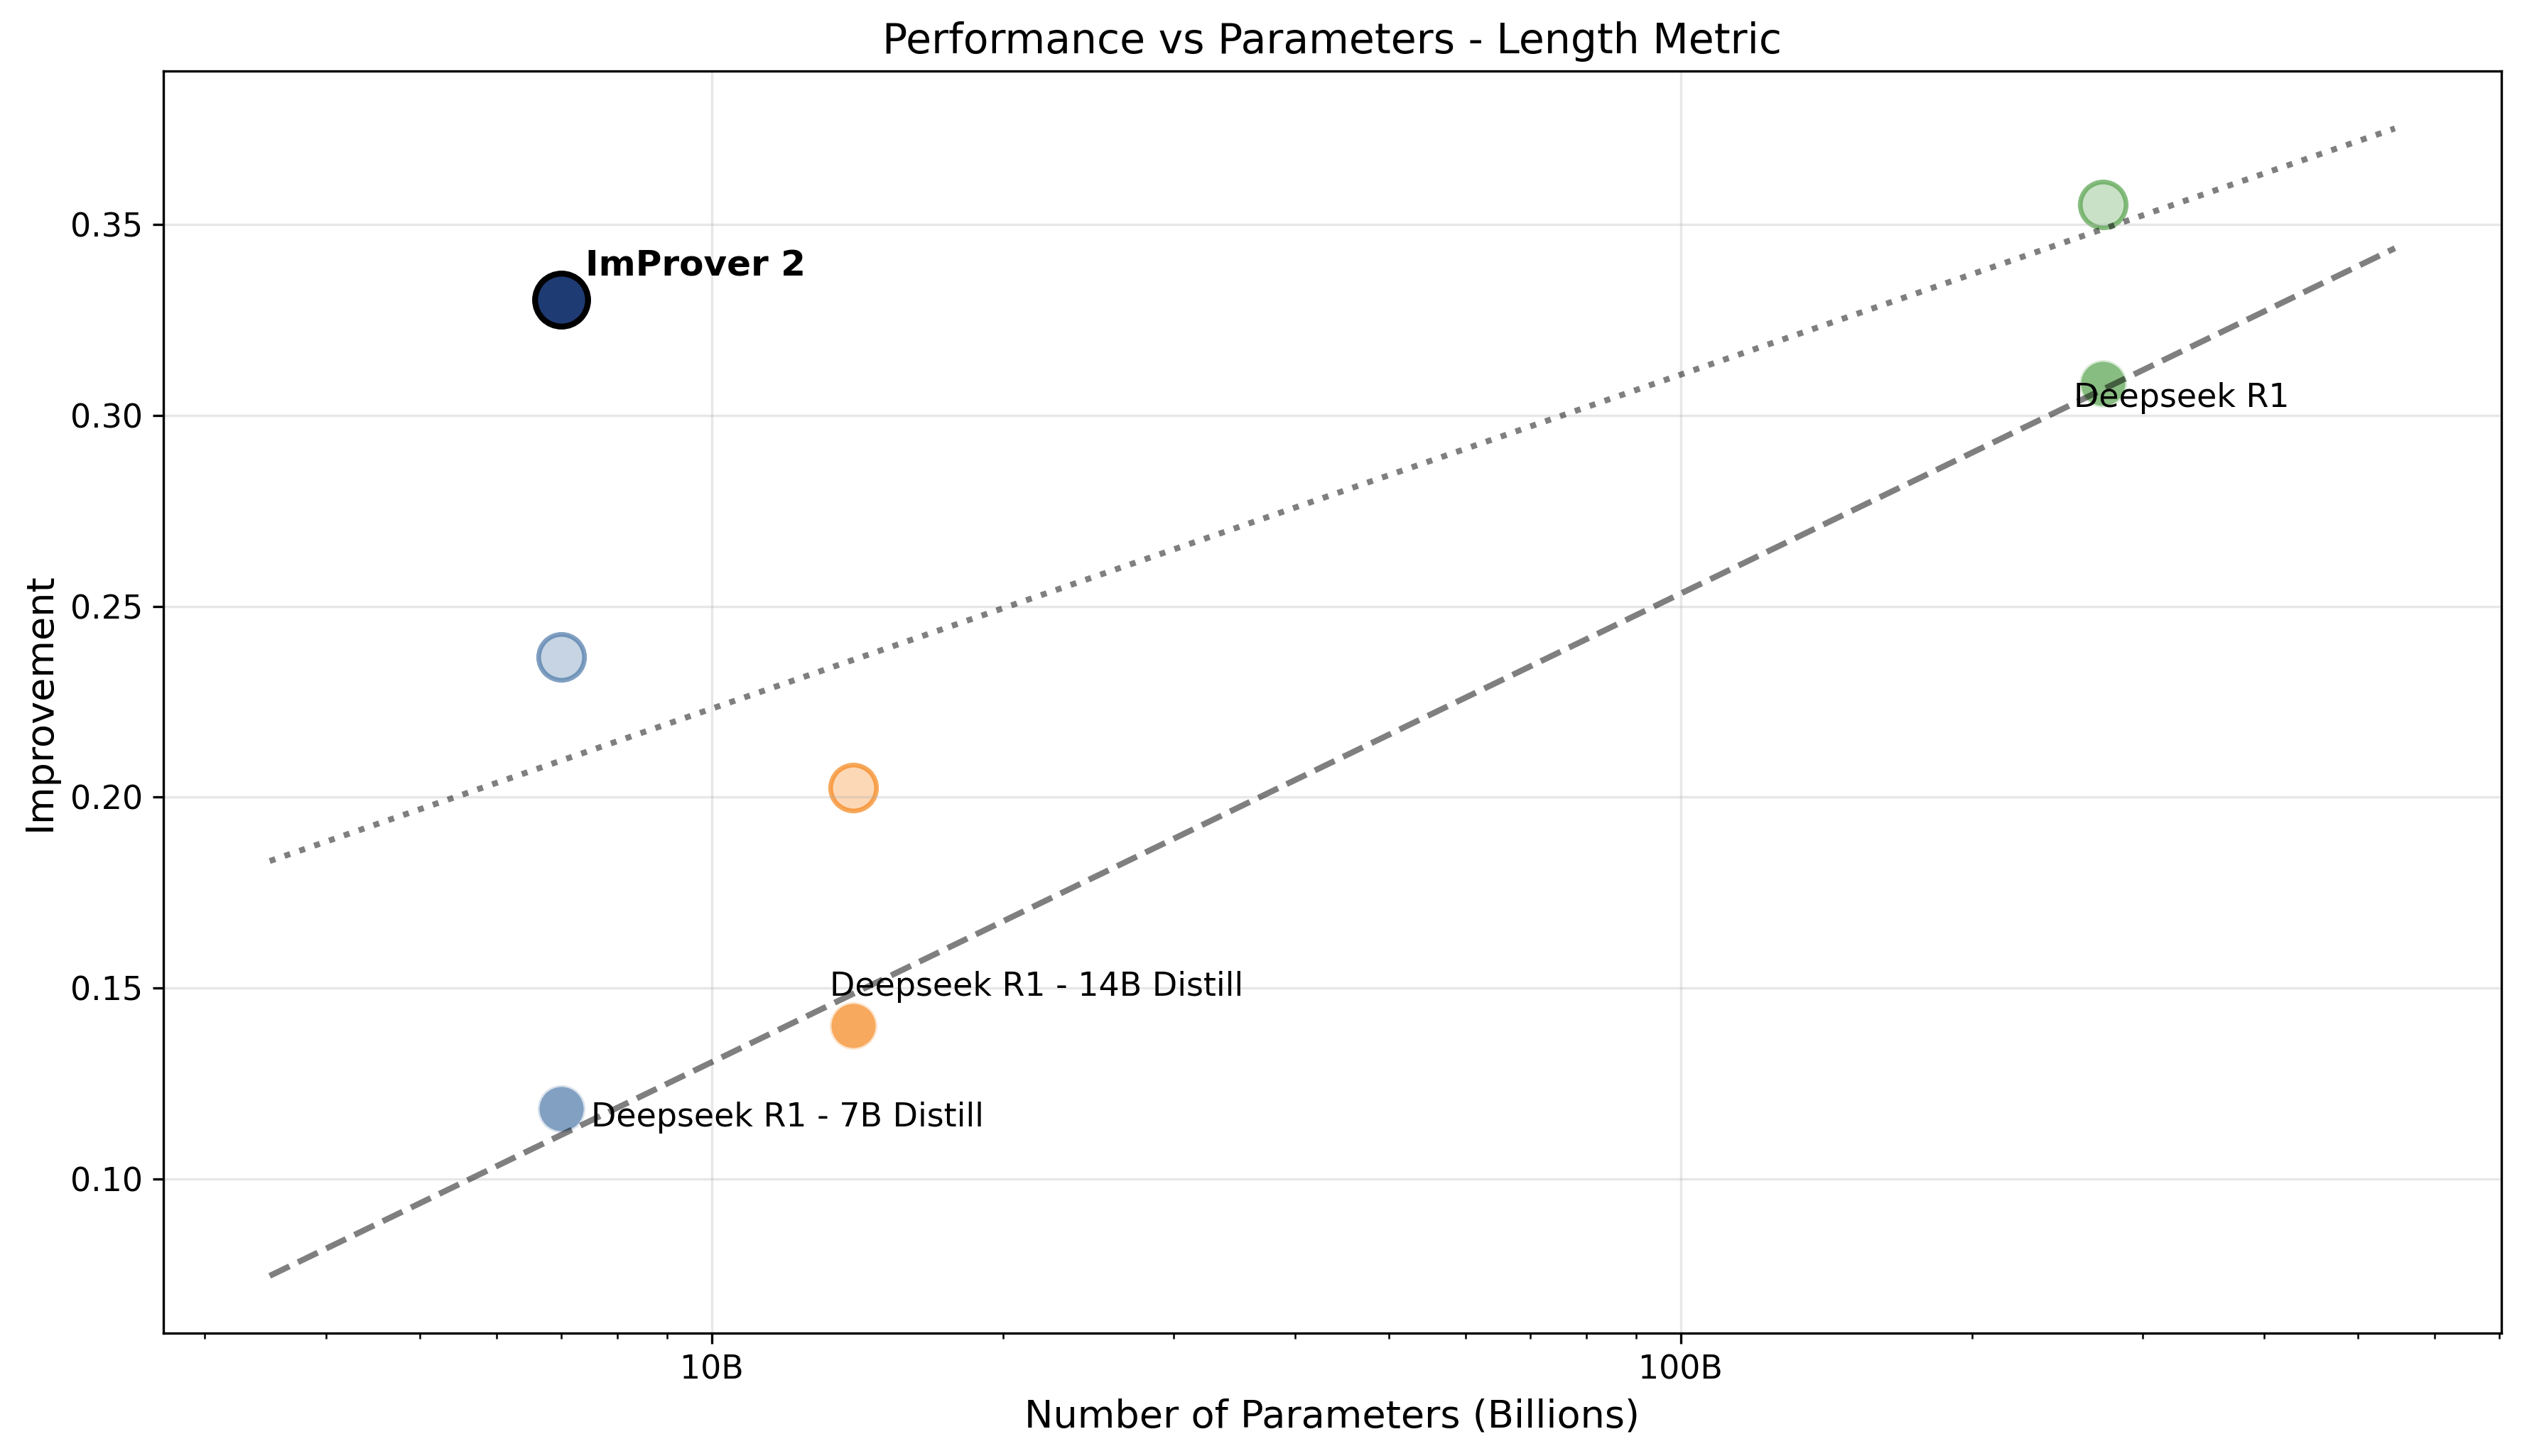
\includegraphics[width=0.82\linewidth]{figures/Length/length_param_perf.png}
\end{center}
\vspace{0.2em}
\small Within DeepSeek family: larger model scores higher. \textbf{ImProver~2 (7B)} outperforms DeepSeek-671B.
\end{frame}

\begin{frame}{Performance vs.\ Parameter Count: Modularity}
\begin{center}
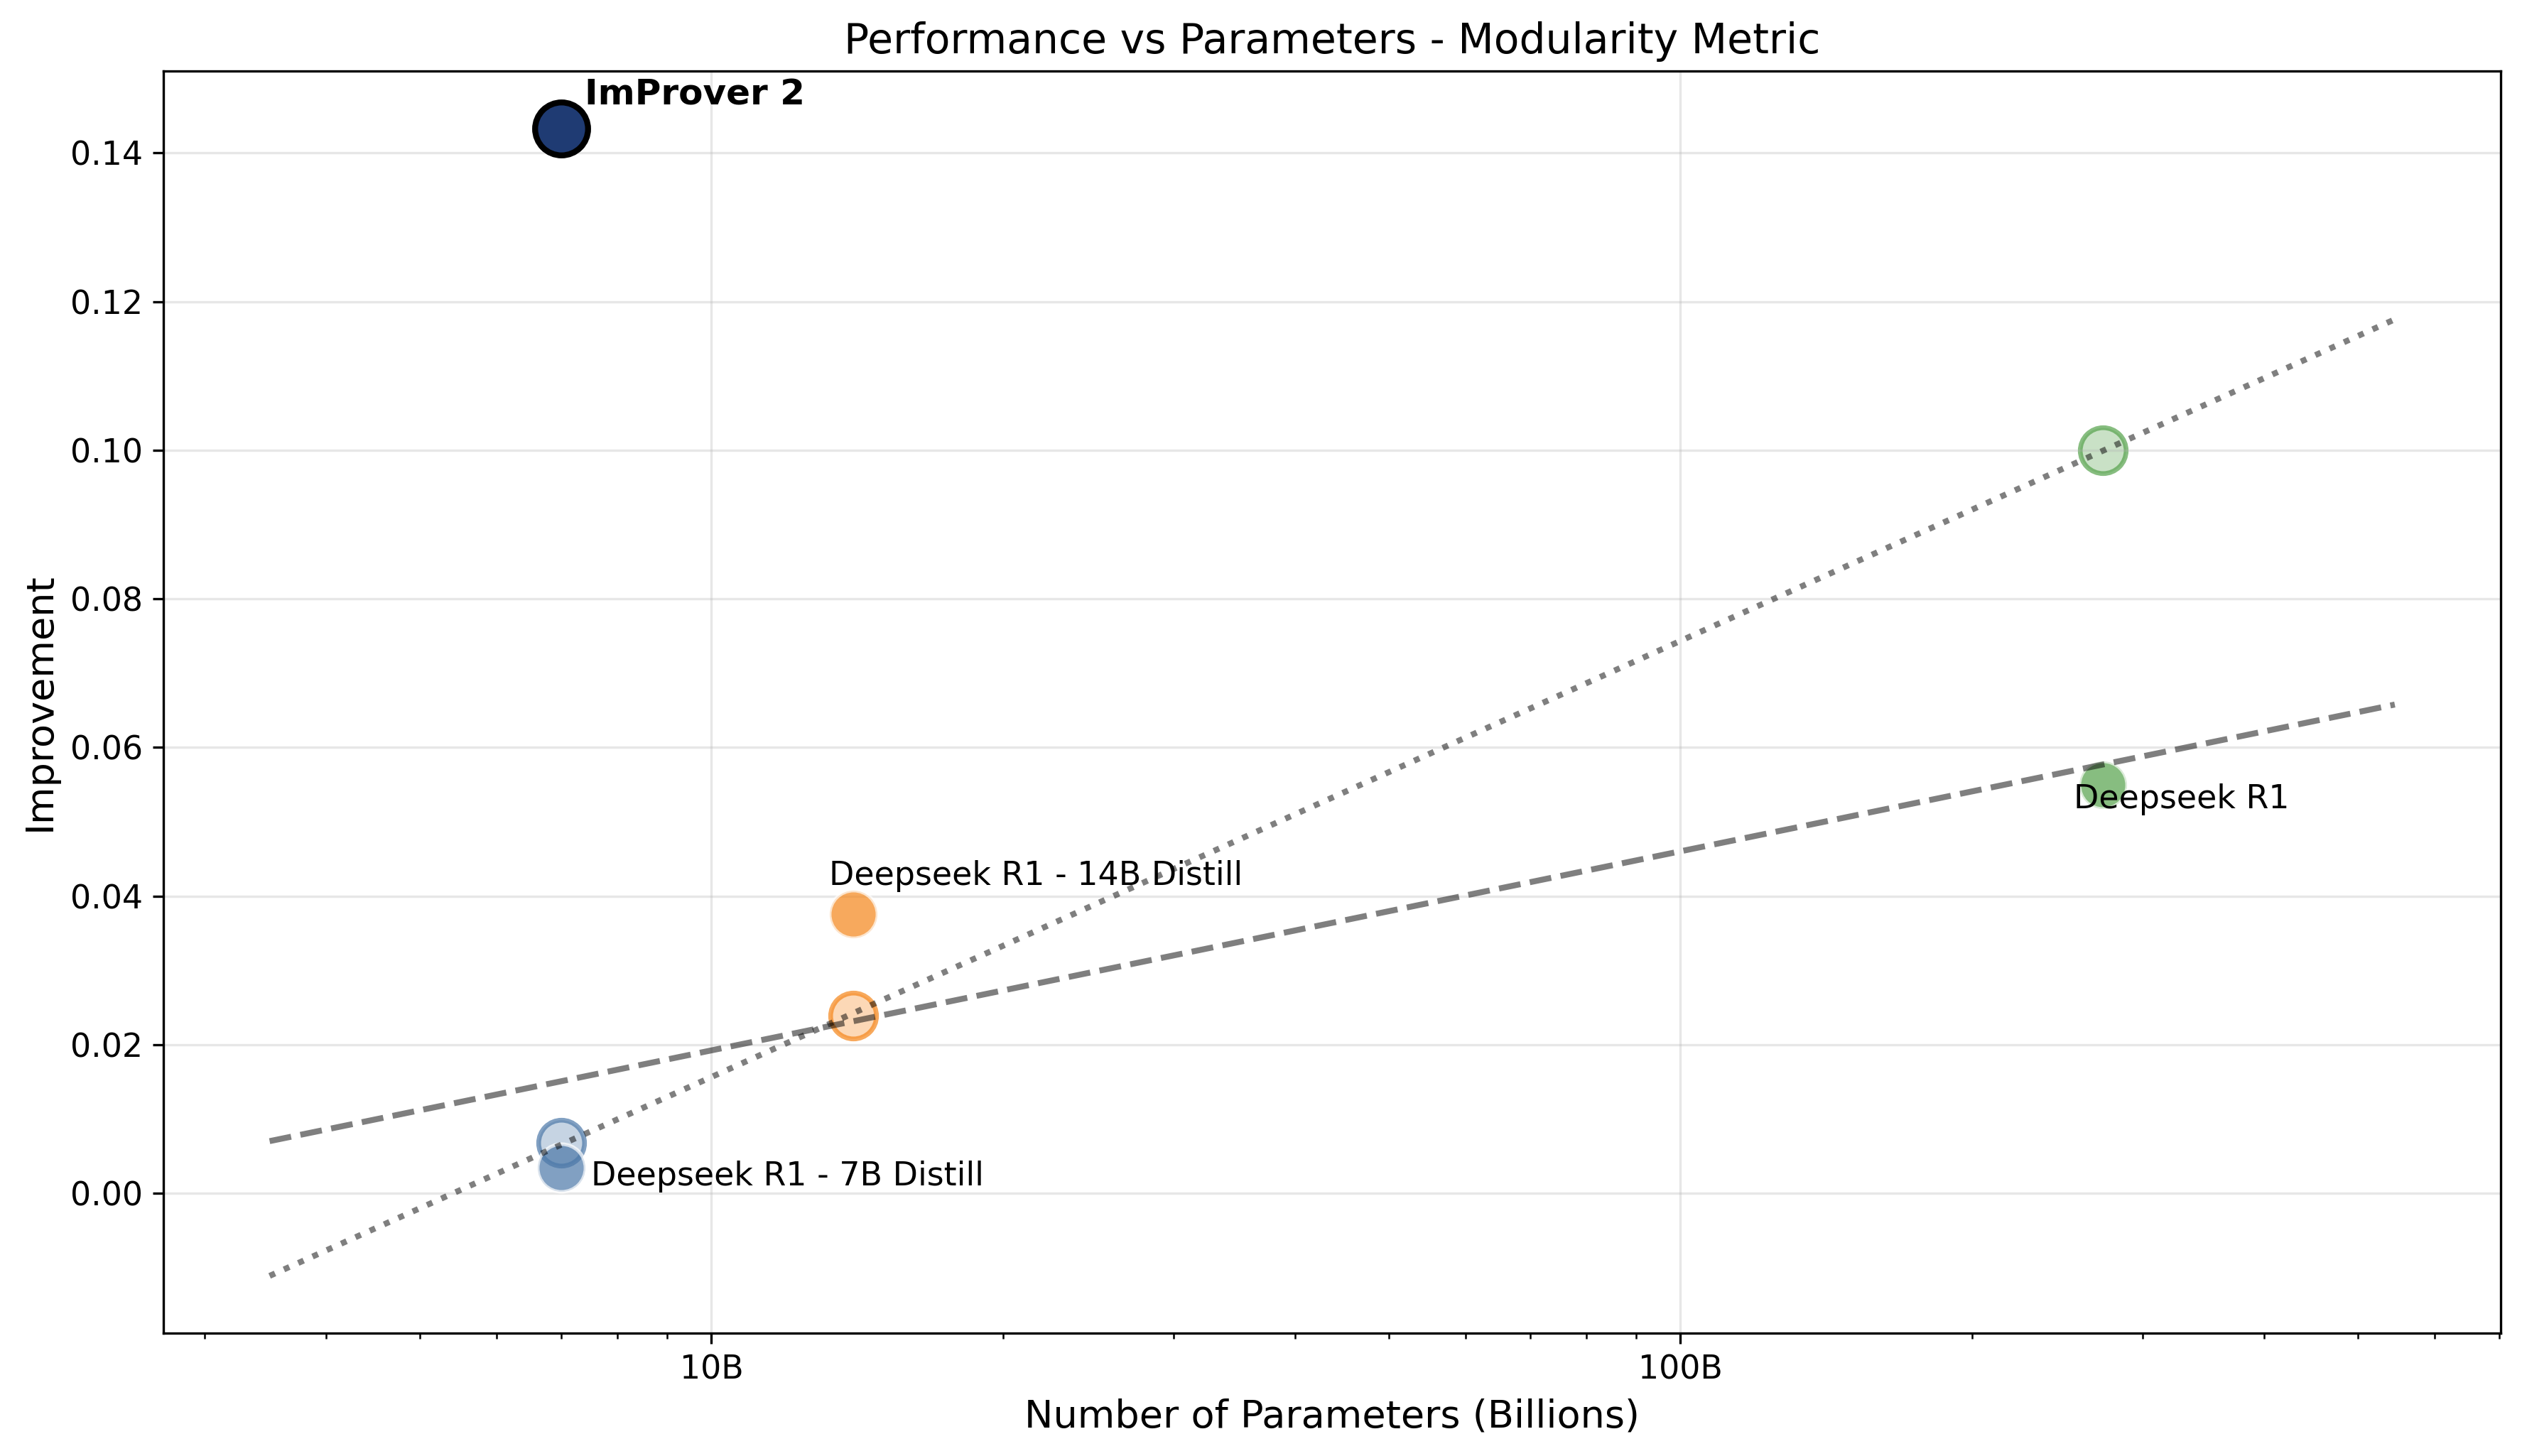
\includegraphics[width=0.82\linewidth]{figures/Modularity/declarativity2_param_perf.png}
\end{center}
\vspace{0.2em}
\small ImProver~2 leads all models on modularity including 671B and GPT-5-high.
\end{frame}

\begin{frame}{Performance vs.\ Parameter Count: Dependencies}
\begin{center}
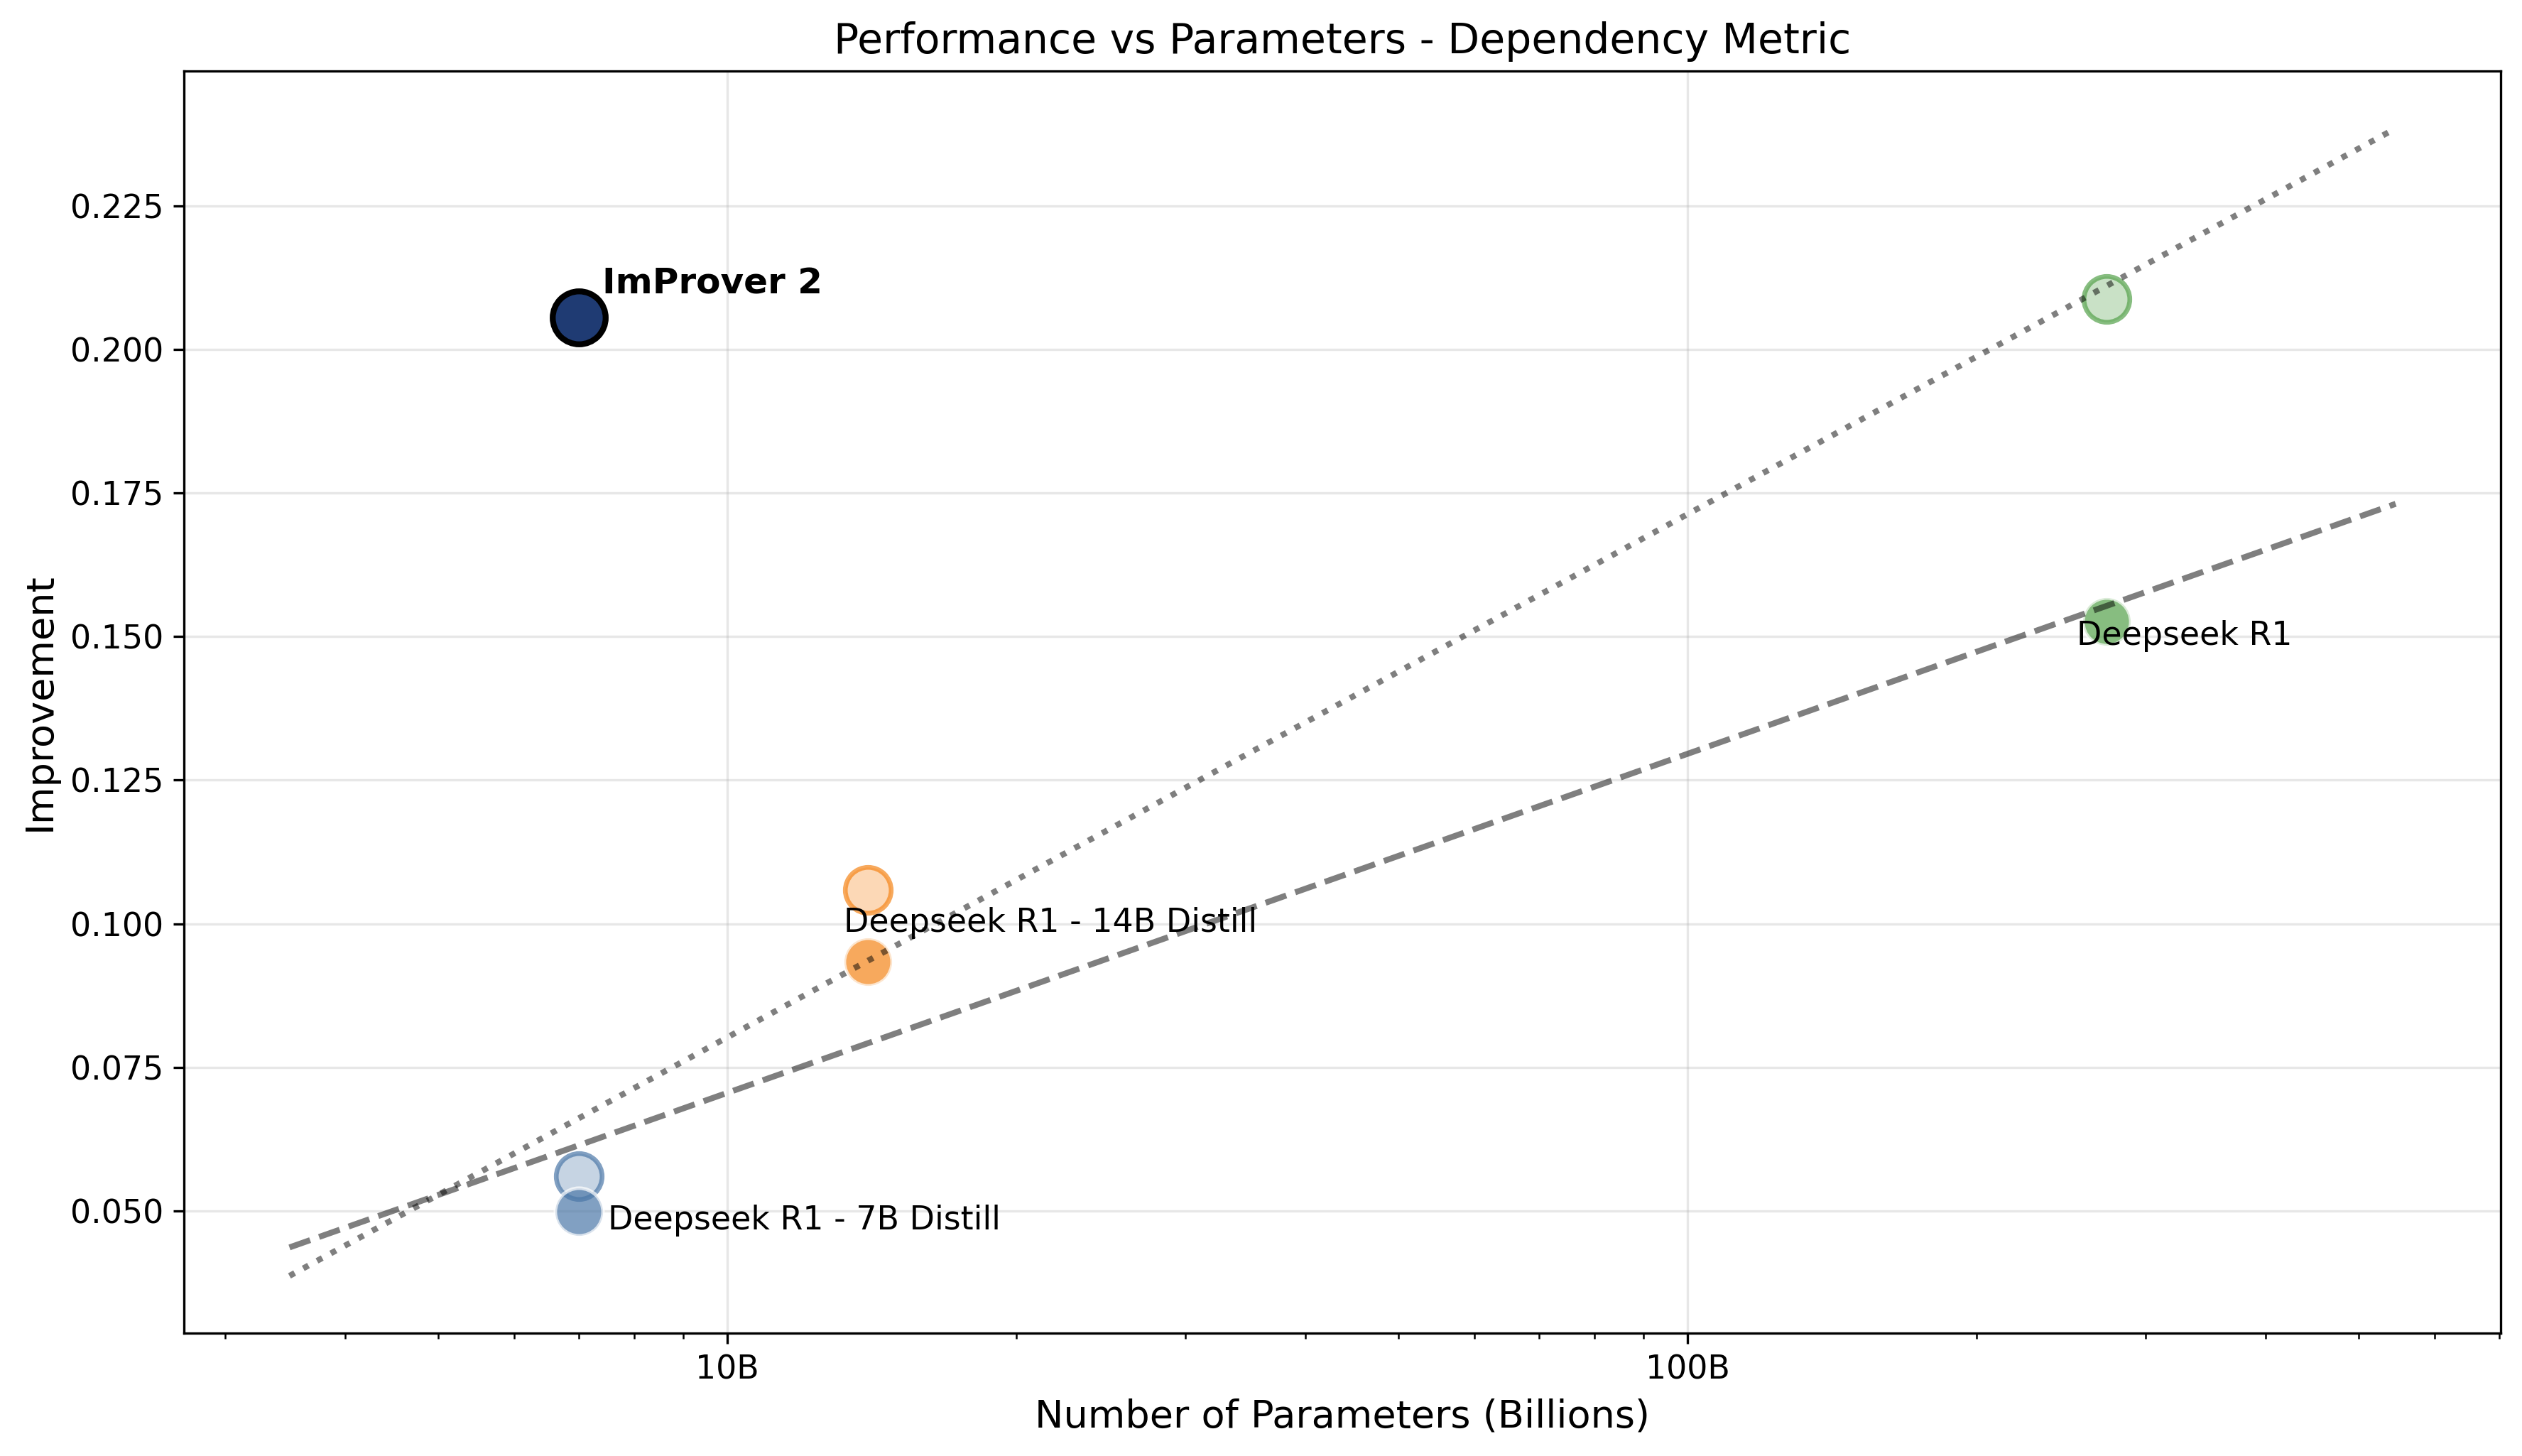
\includegraphics[width=0.82\linewidth]{figures/Dependency/dependency_param_perf.png}
\end{center}
\vspace{0.2em}
\begin{alertblock}{}
  \centering\small \textbf{ImProver~2 (7B)} outperforms DeepSeek-671B on all three metrics. Specialization beats scale.
\end{alertblock}
\end{frame}

\begin{frame}{Full Accuracy and Compilation Breakdown}
\begin{center}
\small ($\mathcal{A}^+_\mu / \mathcal{A}$: improved accuracy / compilation accuracy)\\[0.5em]
\begin{tabular}{l|ccc}
\hline
\textbf{Model} & \textbf{Length} & \textbf{Mod.} & \textbf{Dep.}\\
\hline
DS-R1 7B    & 0.062/0.617 & 0.003/0.570 & 0.037/0.754\\
DS-R1 671B  & 0.162/0.536 & 0.048/0.536 & 0.109/0.480\\
ImProver~2  & 0.131/0.657 & 0.065/0.579 & 0.069/0.368\\
GPT-5-high  & \good{0.264}/\good{0.757} & \good{0.092}/0.656 & 0.094/0.753\\
\hline
\end{tabular}
\end{center}
\vspace{0.3em}
\small ImProver~2 attempts riskier structural transformations; its $\mathcal{A}^+$ is higher relative to its $\mathcal{A}$ than frontier models.
\end{frame}

\begin{frame}{Frontier Comparison: Length (Best@$n$)}
\begin{center}
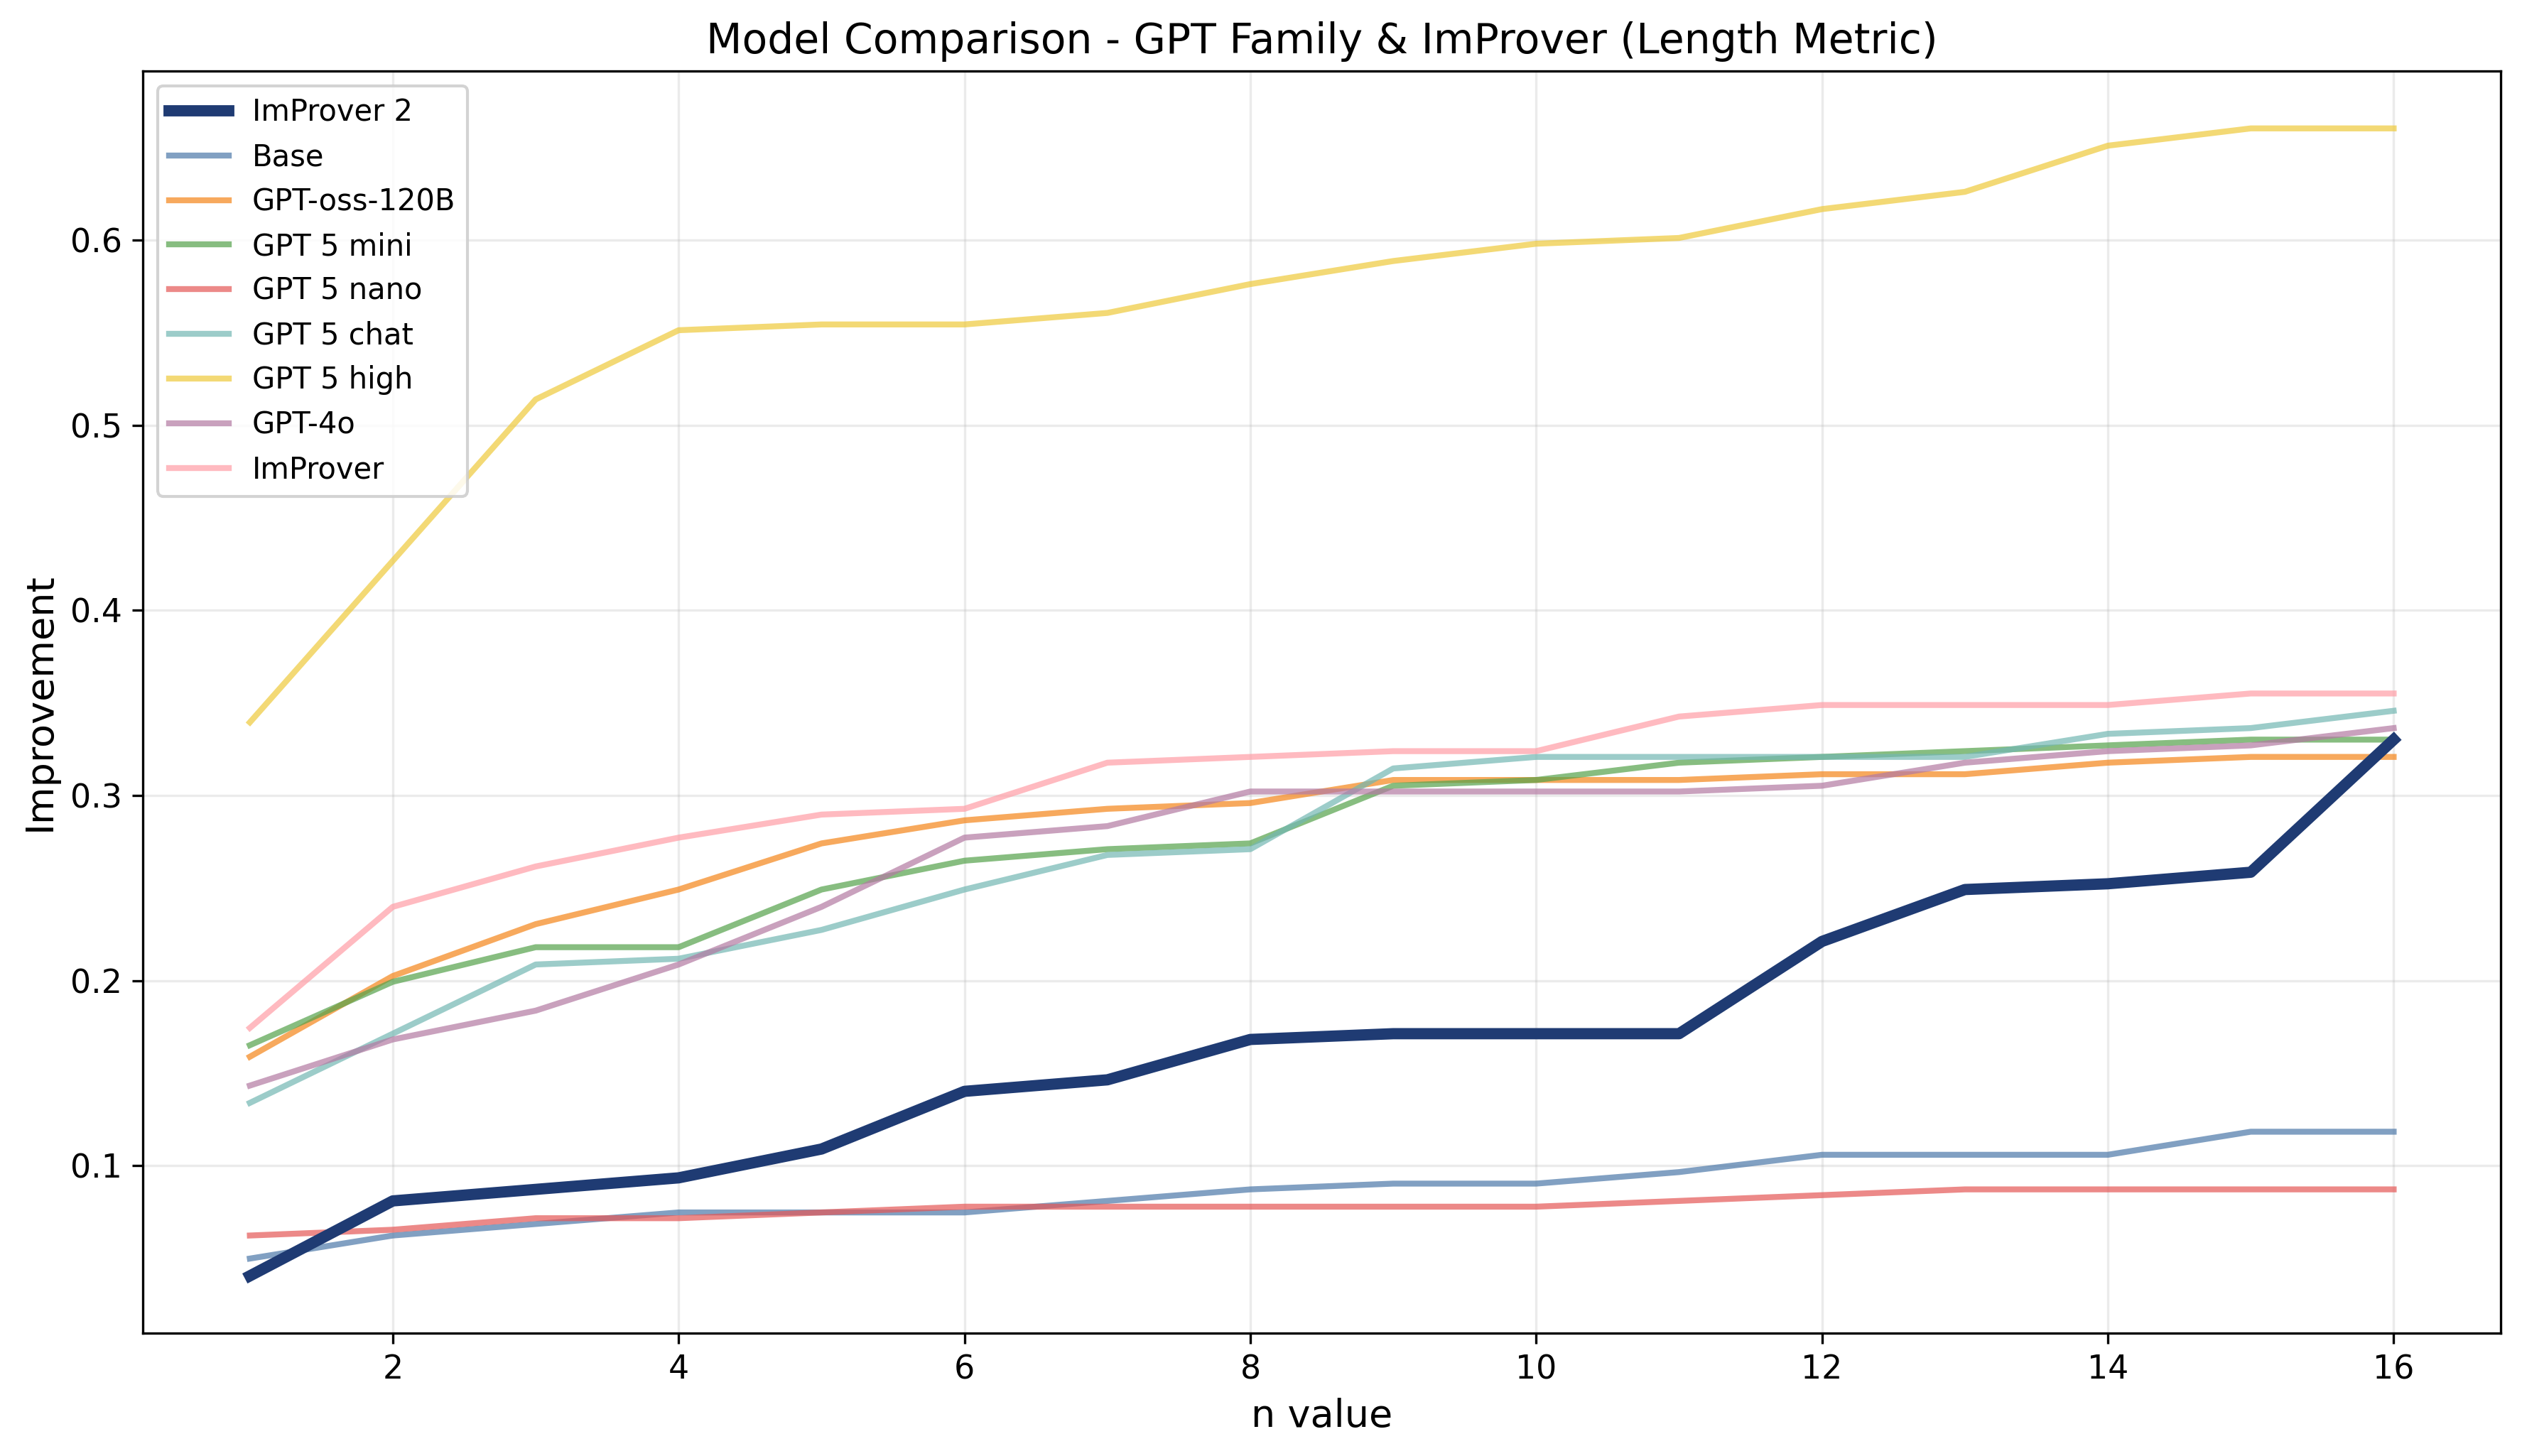
\includegraphics[width=0.82\linewidth]{figures/Length/length_gpt_improver_comparison.png}
\end{center}
\vspace{0.2em}
\small ImProver~2 vs.\ frontier GPT models, best@$n$ ($n=1$--$16$), length metric.
\end{frame}

\begin{frame}{Frontier Comparison: Modularity (Best@$n$)}
\begin{center}
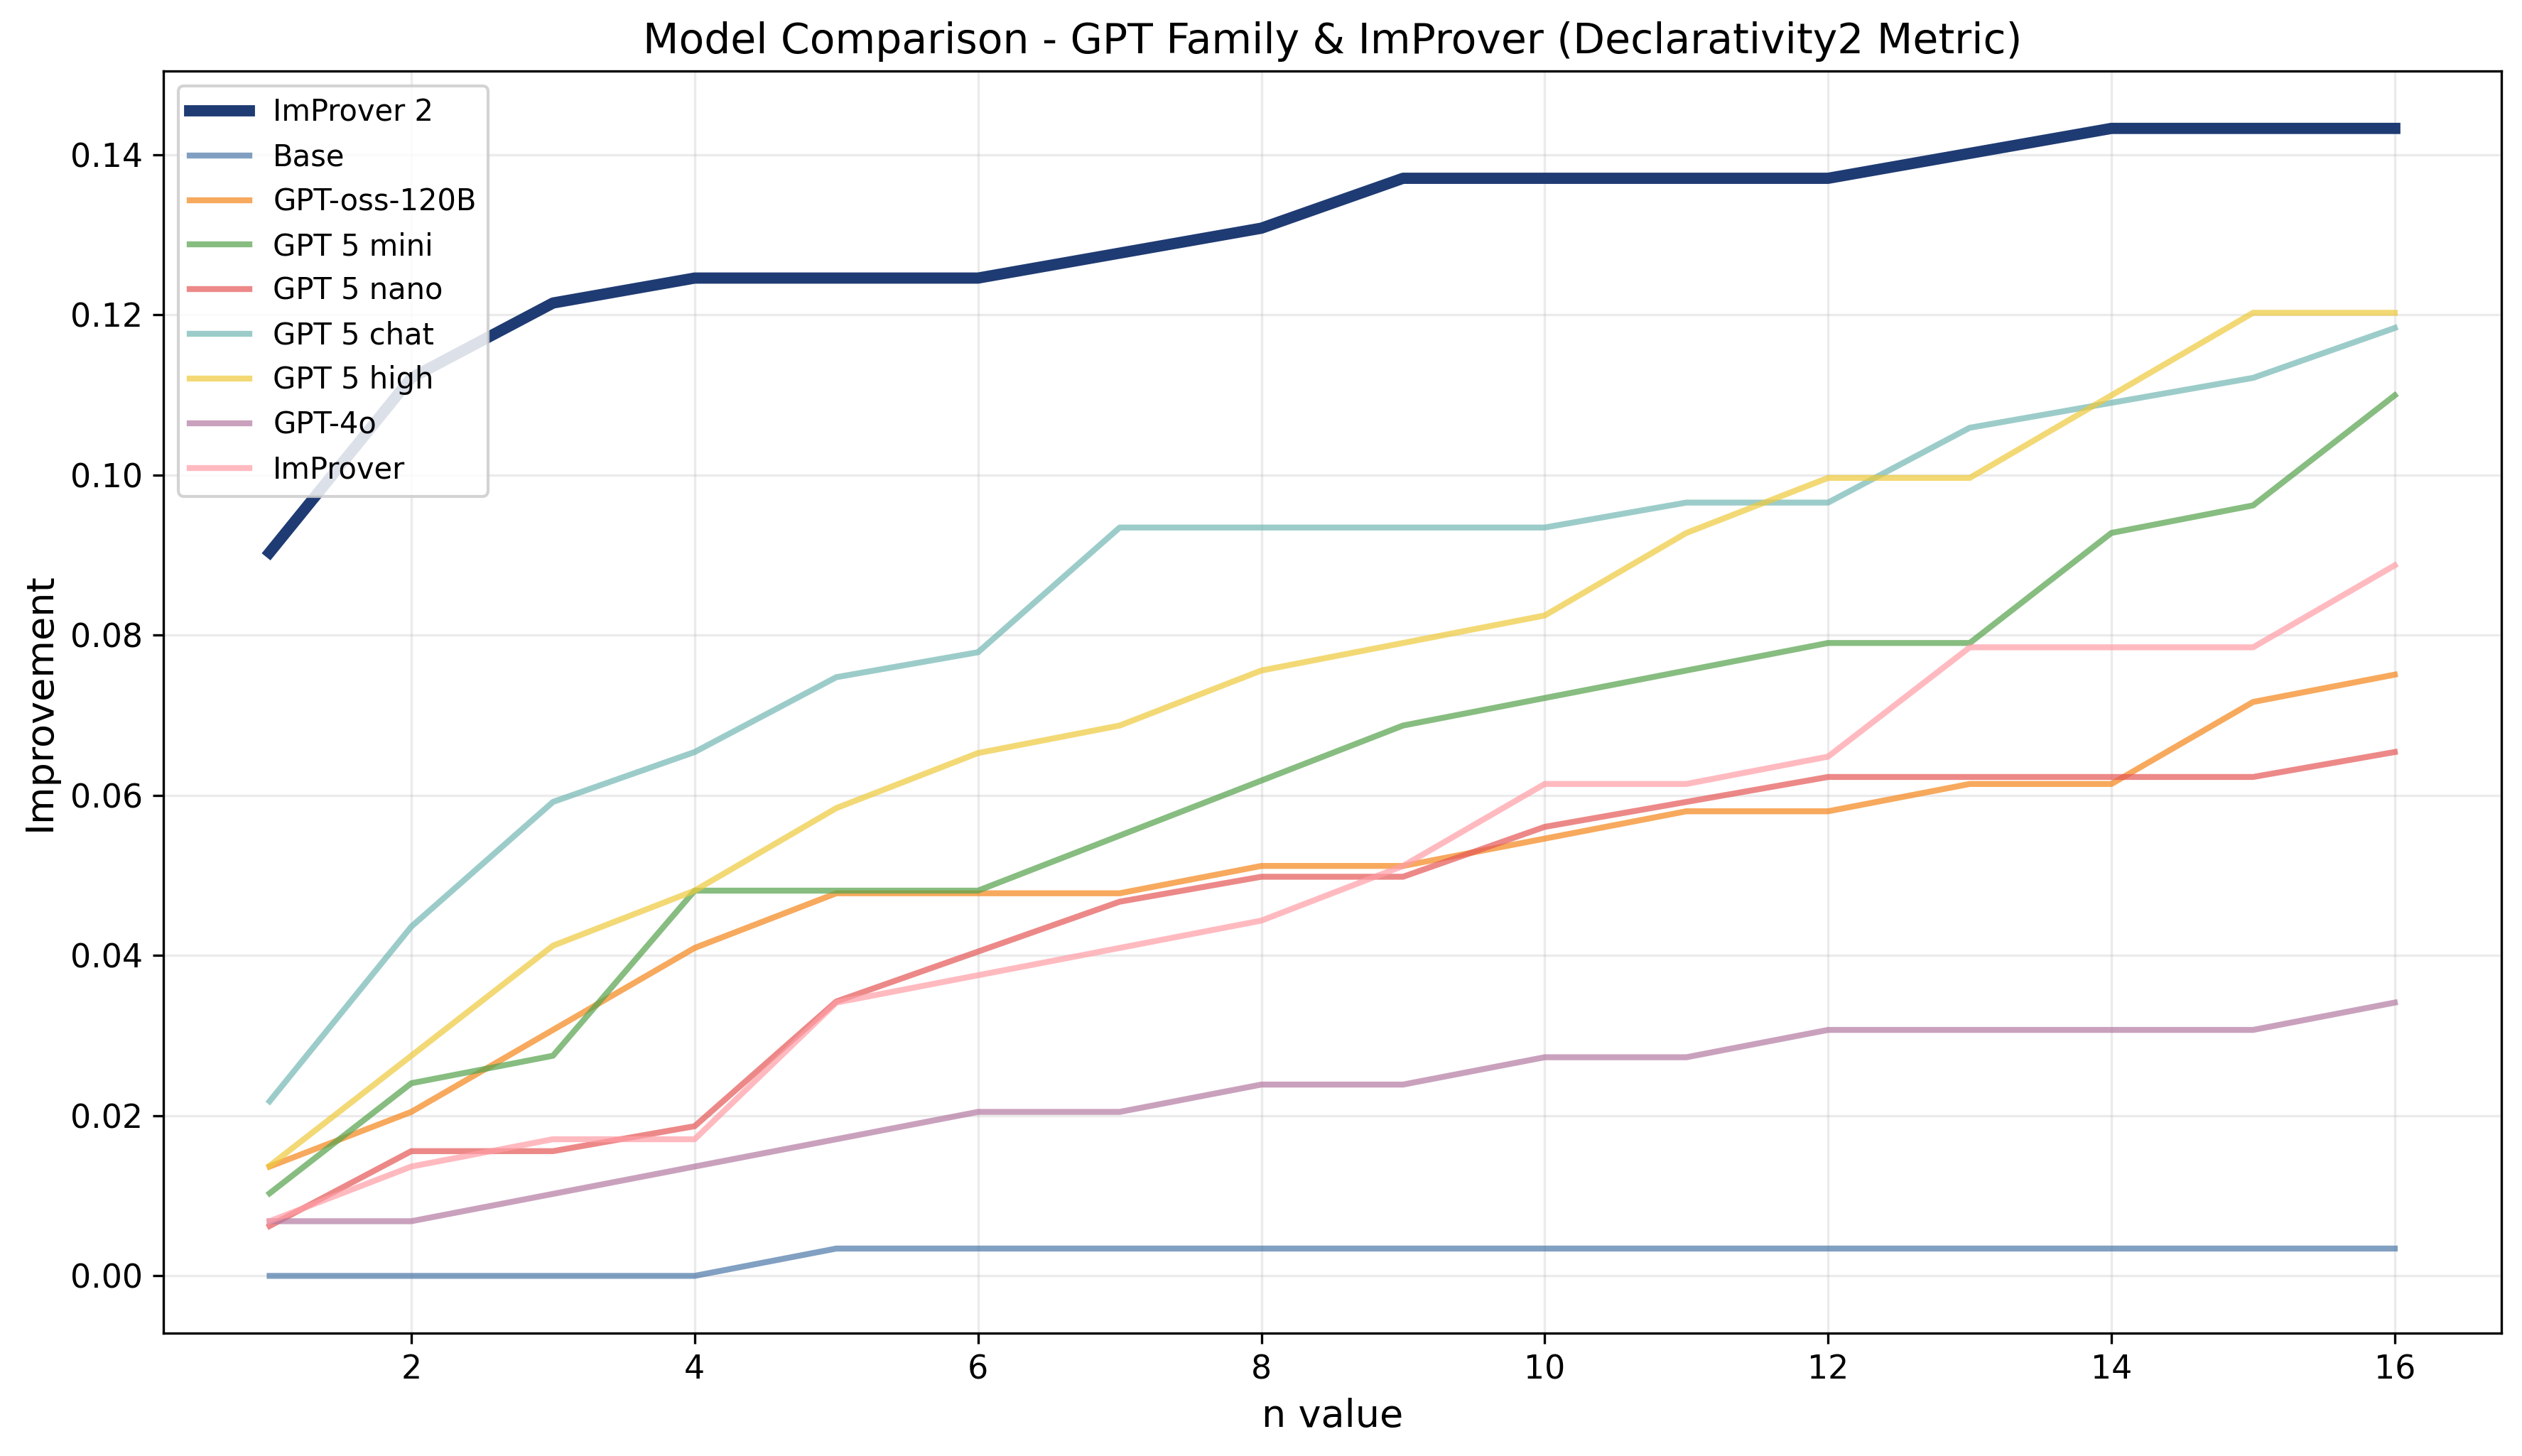
\includegraphics[width=0.82\linewidth]{figures/Modularity/declarativity2_gpt_improver_comparison.png}
\end{center}
\vspace{0.2em}
\small ImProver~2 leads all models on modularity at every $n$, including GPT-5-high.
\end{frame}

\begin{frame}{Frontier Comparison: Dependencies (Best@$n$)}
\begin{center}
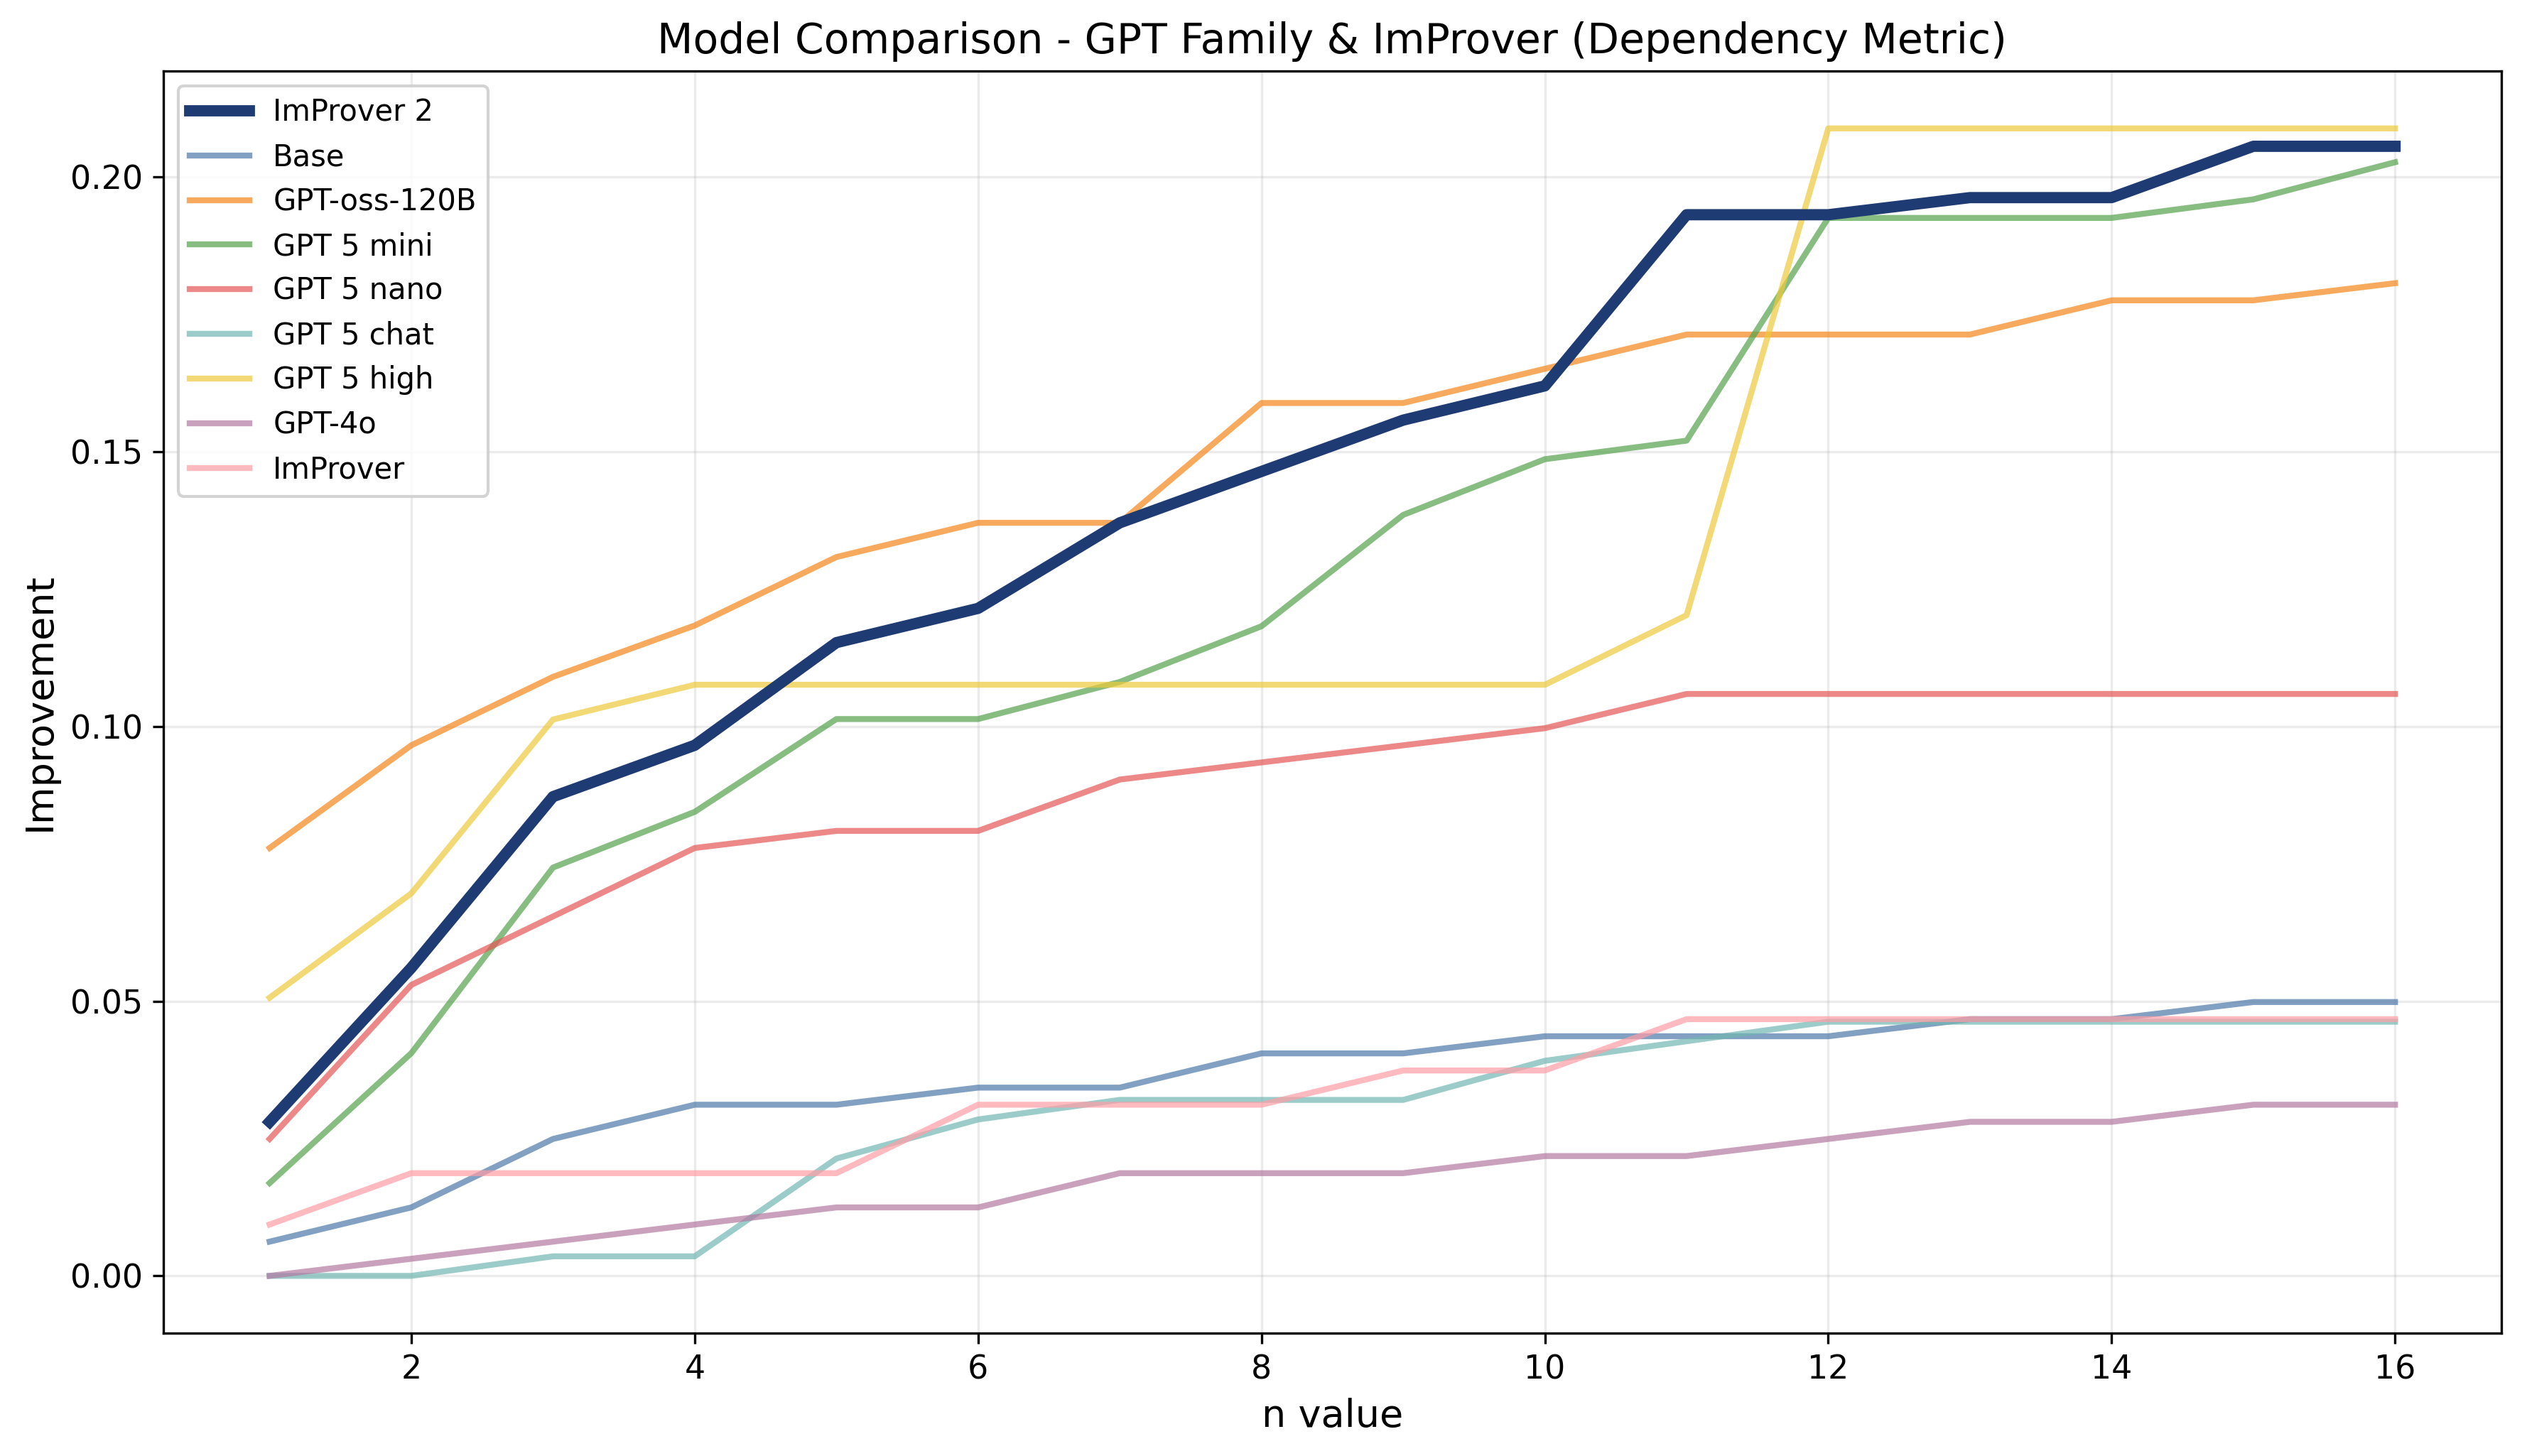
\includegraphics[width=0.82\linewidth]{figures/Dependency/dependency_gpt_improver_comparison.png}
\end{center}
\vspace{0.2em}
\small Competitive with frontier on dependencies; gap narrows at higher $n$.
\end{frame}

\begin{frame}{Effect of Neurosymbolic Scaffold}
\vspace{0.2em}
\begin{center}
\resizebox{\linewidth}{!}{%
\small
\begin{tabular}{llccccccccc}
\toprule
\textbf{Metric} & \textbf{Variant} & \textbf{DS-R1 7B} & \textbf{DS-R1 14B} & \textbf{DS-R1 671B} & \textbf{GPT-4o} & \textbf{GPT-oss} & \textbf{GPT-5-nano} & \textbf{GPT-5-mini} & \textbf{GPT-5-chat} & \textbf{GPT-5-high}\\
\midrule
\multirow{2}{*}{Length} & Base & 0.118 & 0.140 & 0.308 & 0.336 & 0.321 & 0.087 & 0.330 & 0.346 & 0.660\\
 & Scaffold & \textbf{0.236} & \textbf{0.202} & \textbf{0.355} & \textbf{0.396} & \textbf{0.508} & \textbf{0.296} & \textbf{0.632} & \textbf{0.576} & \textbf{0.875}\\
\midrule
\multirow{2}{*}{Mod.} & Base & 0.003 & \textbf{0.037} & 0.055 & 0.034 & 0.075 & 0.065 & 0.109 & 0.118 & 0.120\\
 & Scaffold & \textbf{0.007} & 0.024 & \textbf{0.100} & \textbf{0.092} & \textbf{0.092} & \textbf{0.069} & \textbf{0.123} & \textbf{0.153} & ---\\
\midrule
\multirow{2}{*}{Dep.} & Base & 0.050 & 0.093 & 0.153 & 0.050 & 0.181 & 0.106 & 0.203 & 0.046 & 0.208\\
 & Scaffold & \textbf{0.056} & \textbf{0.106} & \textbf{0.209} & \textbf{0.075} & \textbf{0.406} & \textbf{0.108} & \textbf{0.267} & \textbf{0.087} & \textbf{0.315}\\
\bottomrule
\end{tabular}%
}
\end{center}
\vspace{0.3em}
\small Scaffold improves nearly all models on all metrics. DS-R1-7B length: $0.118 \to 0.236$ (doubles before any training). GPT-5-high: $0.660 \to 0.875$. Gains do \emph{not} diminish with scale.
\end{frame}

\begin{frame}{Scaffold Ablation: Each Channel Contributes}
\begin{center}
\begin{figure}
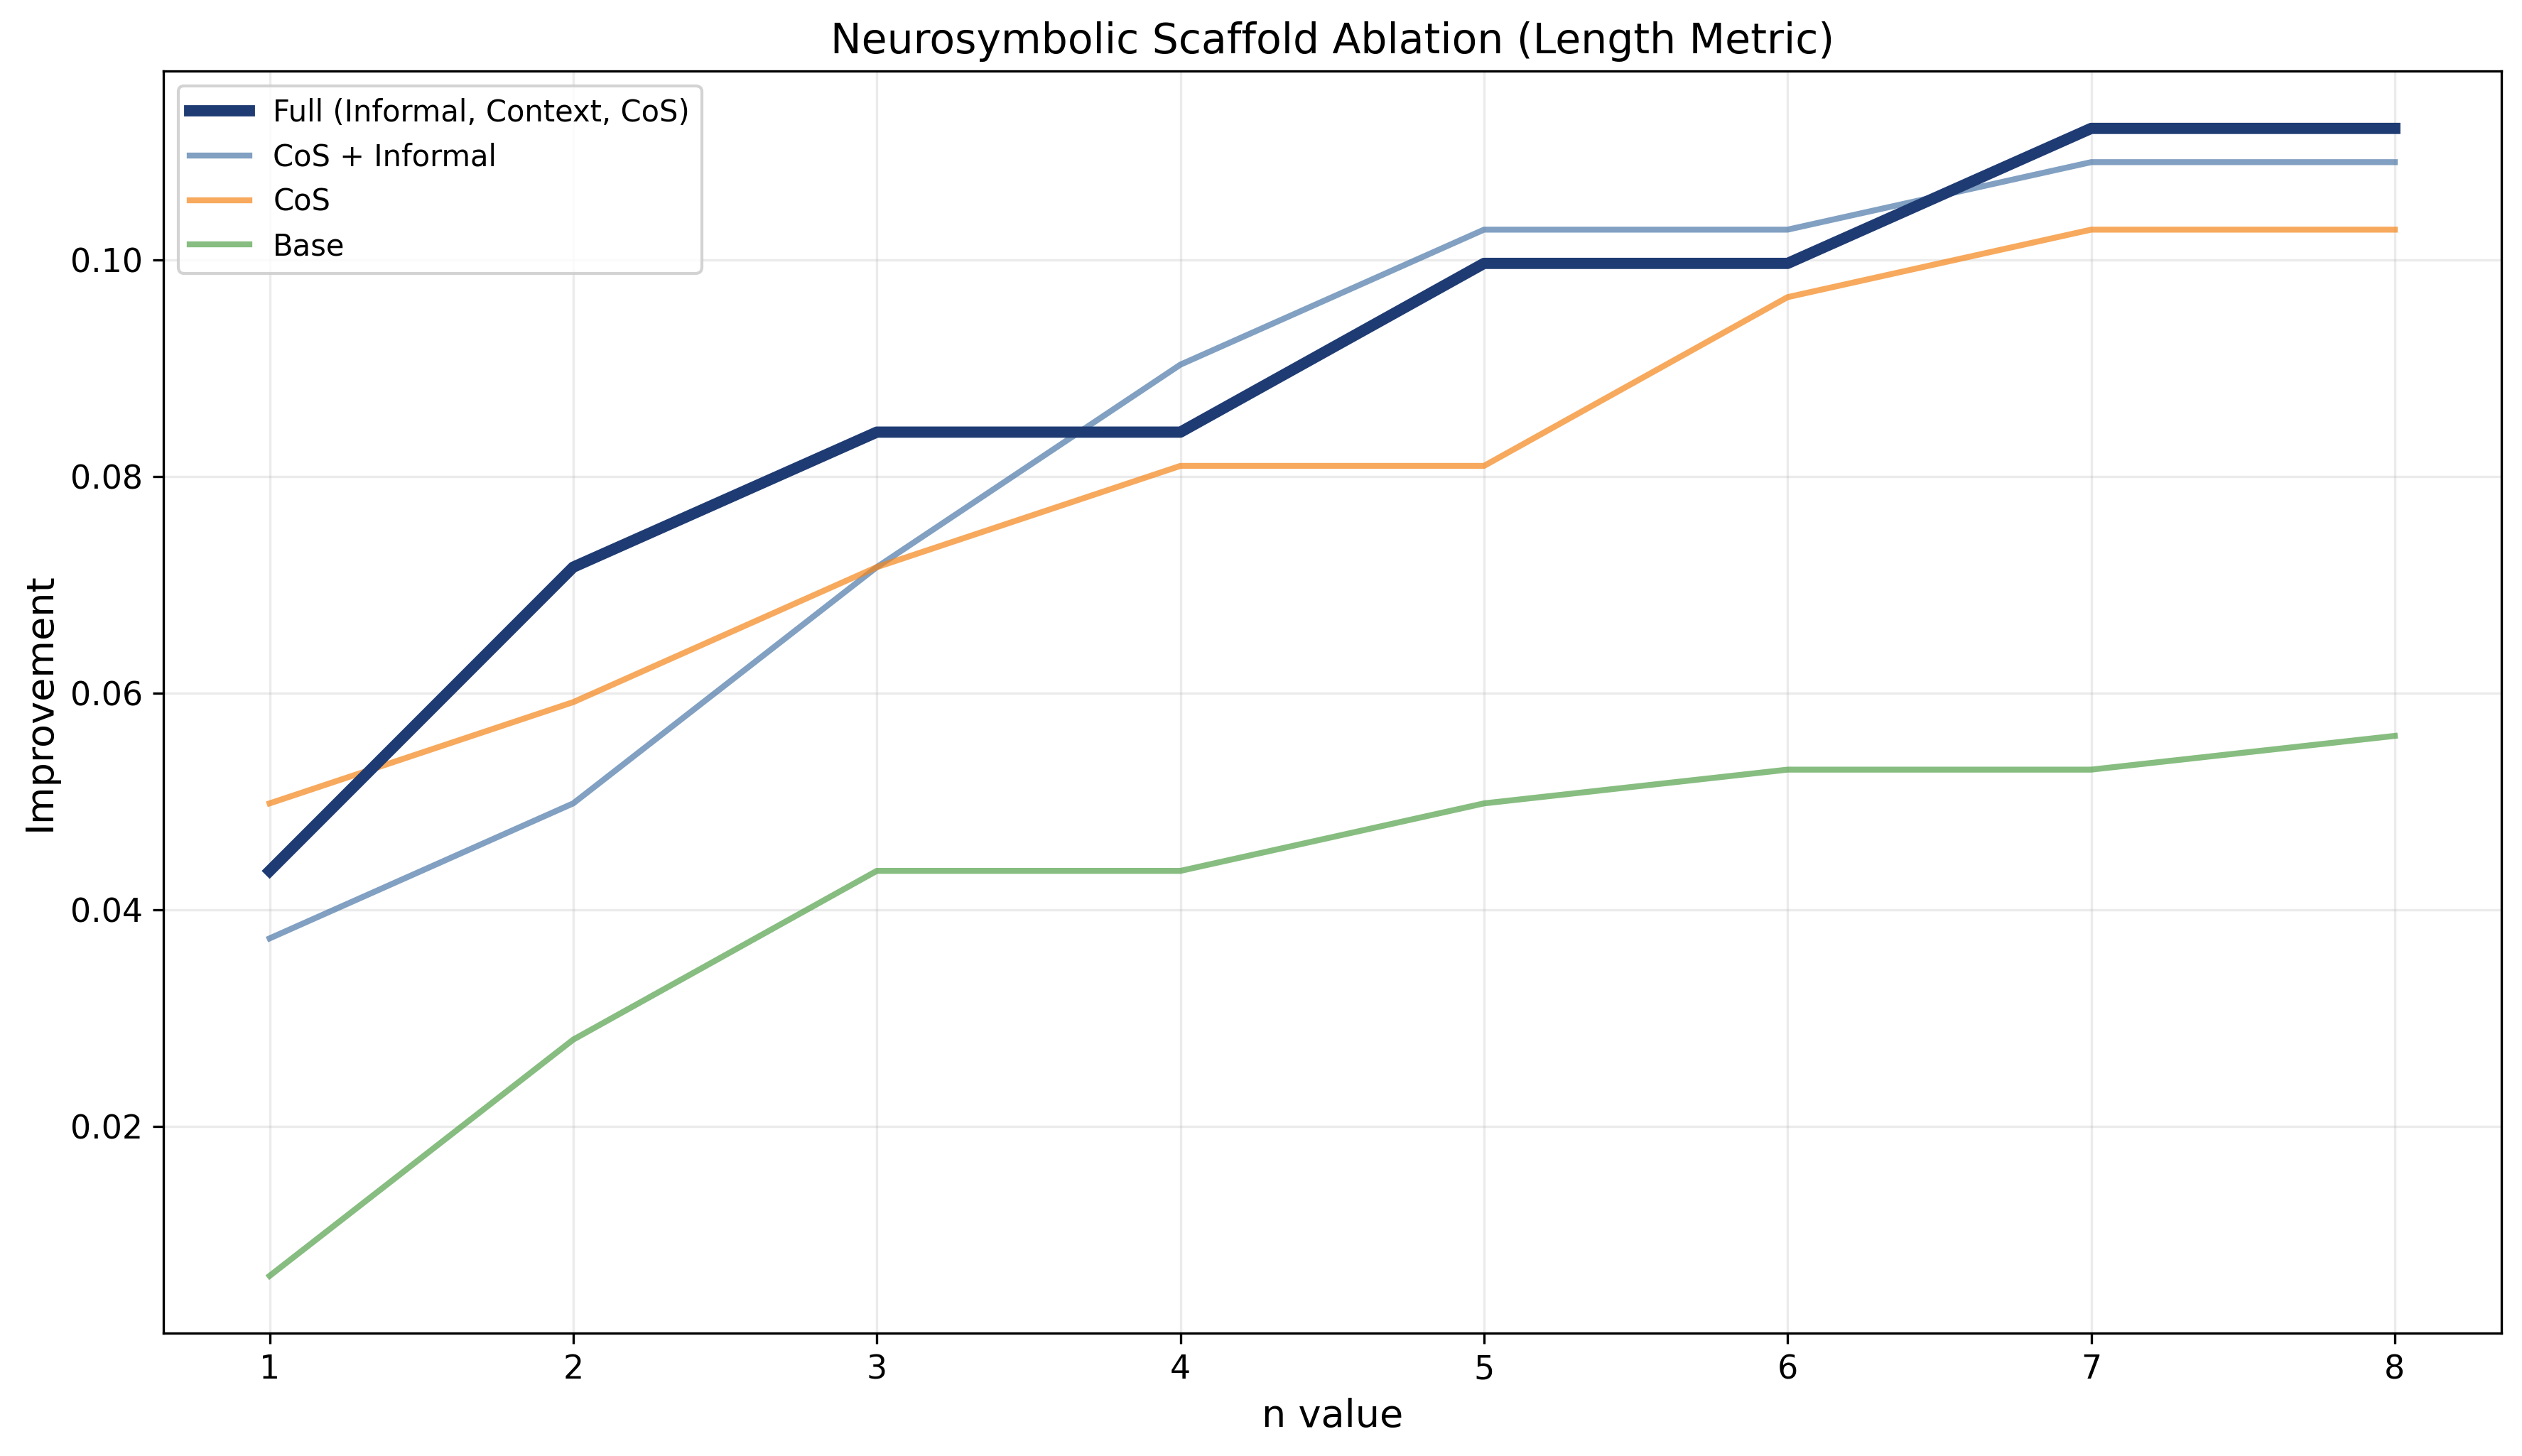
\includegraphics[width=0.85\linewidth]{figures/Length/length_neuro_ablation.png}
\end{figure}
\end{center}
\vspace{0.2em}
\small Each channel (context slice, CoS, auto-informalization) adds incremental improvement on DS-R1-7B (length metric). Adding each source shows noticeable gains on some $n$ values. Diminishing returns as all three are combined.
\end{frame}

\begin{frame}{Training and Iteration Results}
\begin{columns}[T]
\begin{column}{0.52\textwidth}
\begin{figure}
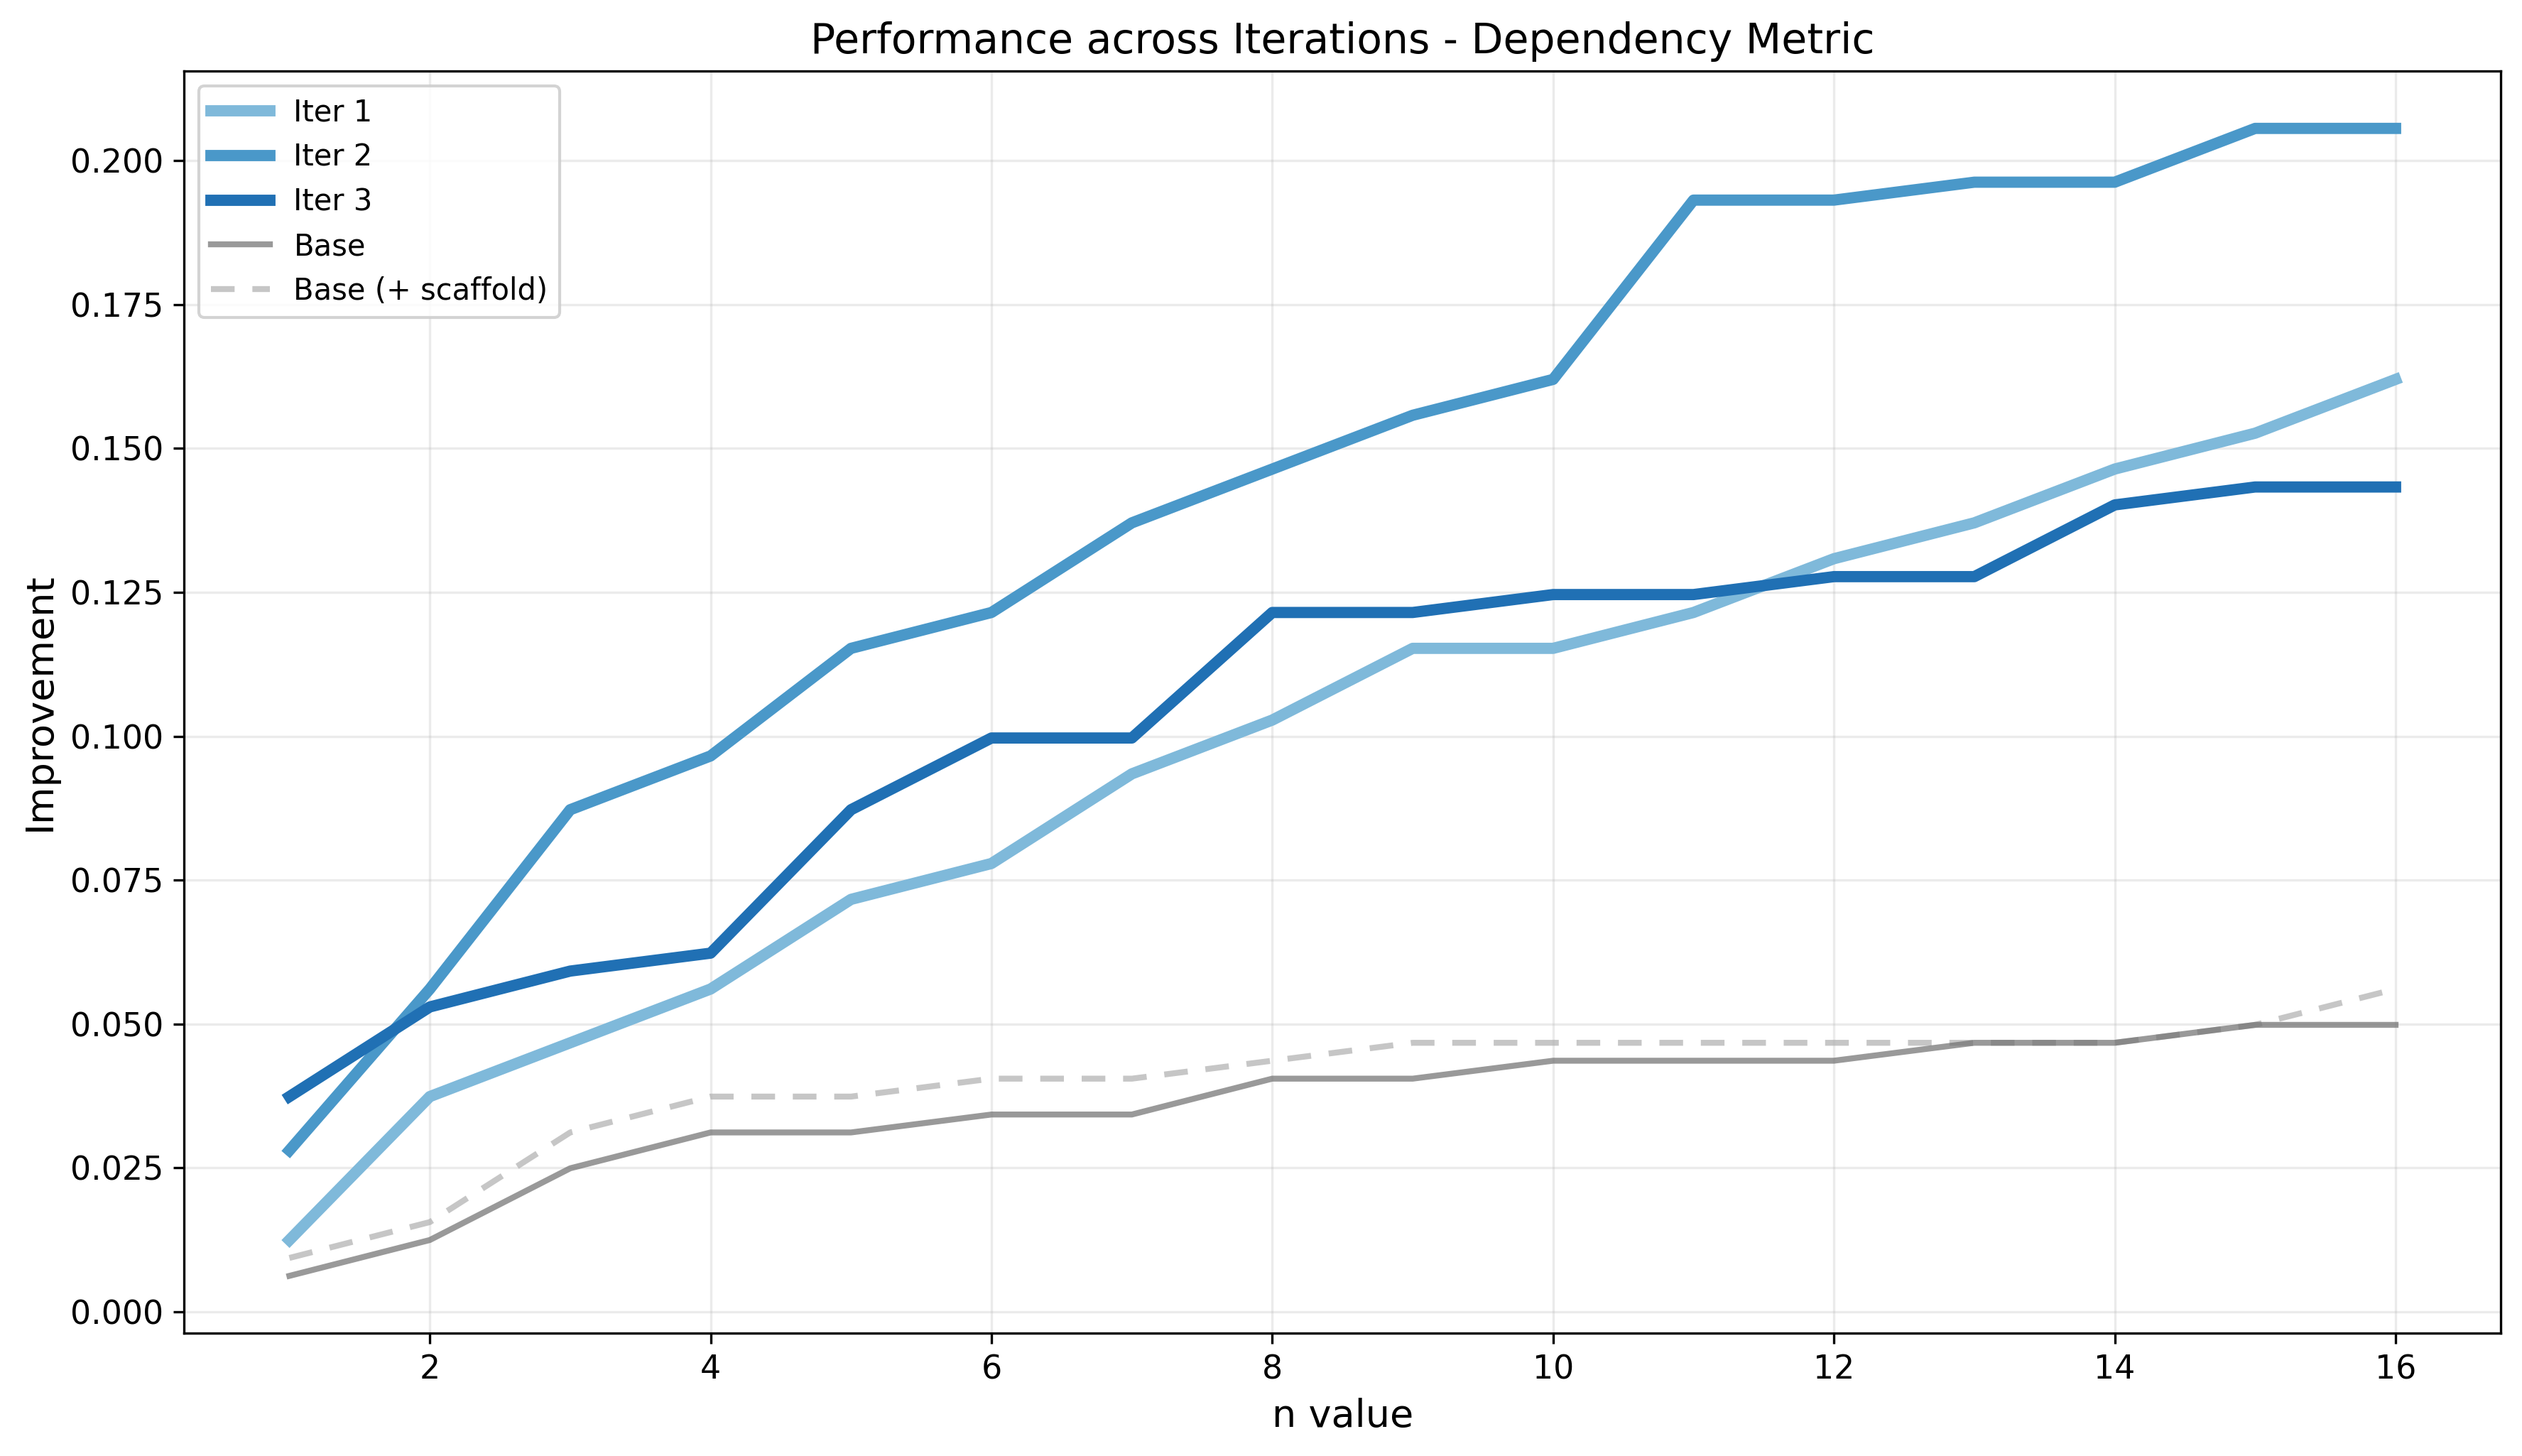
\includegraphics[width=\linewidth]{figures/Dependency/dependency_iterations.png}
\end{figure}
\end{column}
\begin{column}{0.44\textwidth}
\vspace{0.2em}
\resizebox{\columnwidth}{!}{%
\begin{tabular}{l|ccc}
\hline
\textbf{Iter.} & \textbf{Len} & \textbf{Mod} & \textbf{Dep}\\
\hline
Base      & 0.118 & 0.003 & 0.050\\
+Scaffold & 0.236 & 0.007 & 0.056\\
\hdashline
1         & 0.265 & 0.062 & 0.137\\
2         & 0.318 & 0.134 & \good{0.206}\\
3         & \good{0.330} & \good{0.143} & 0.165\\
4         & 0.299 & 0.096 & ---\\
\hline
\end{tabular}%
}
\vspace{0.4em}
\begin{minipage}{\columnwidth}\small Rapid gains in rounds 1--2. Each metric peaks separately. Round 4: regression = saturation.\end{minipage}
\end{column}
\end{columns}
\end{frame}

\begin{frame}{Training Iteration: Modularity and Length}
\begin{columns}[T]
\begin{column}{0.49\textwidth}
\begin{figure}
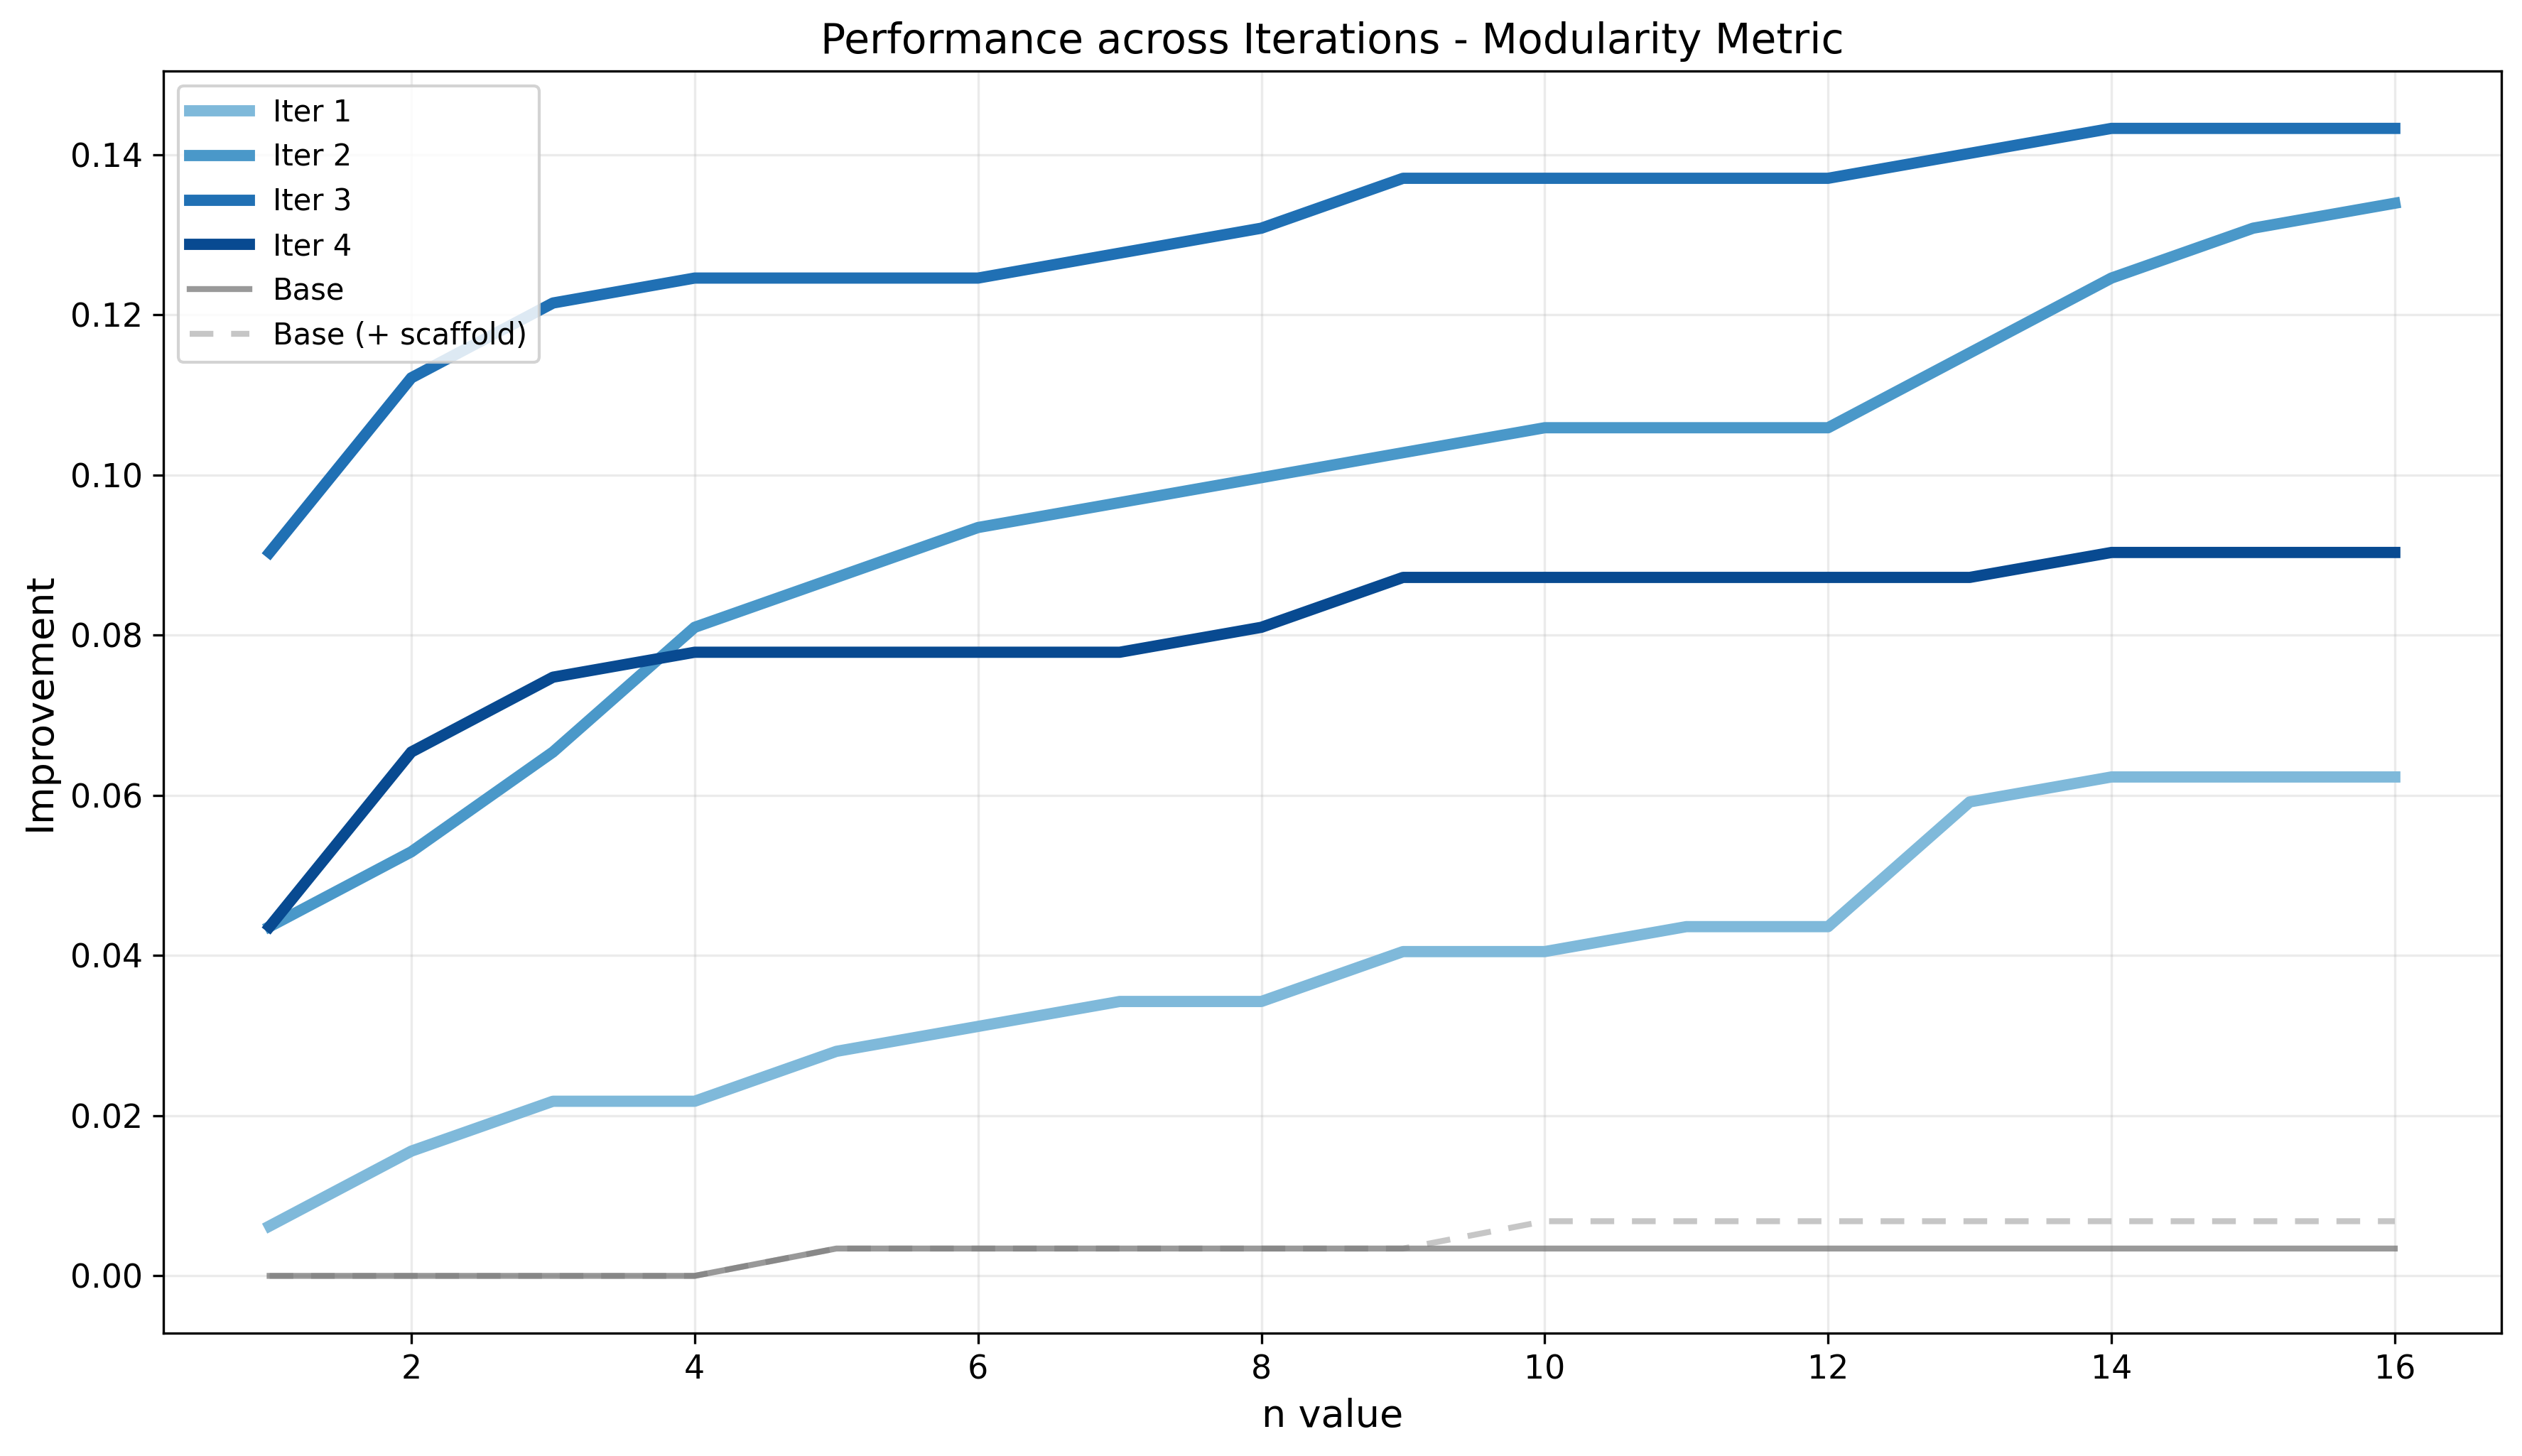
\includegraphics[width=\linewidth]{figures/Modularity/declarativity2_iterations.png}
\end{figure}
\end{column}
\begin{column}{0.49\textwidth}
\begin{figure}
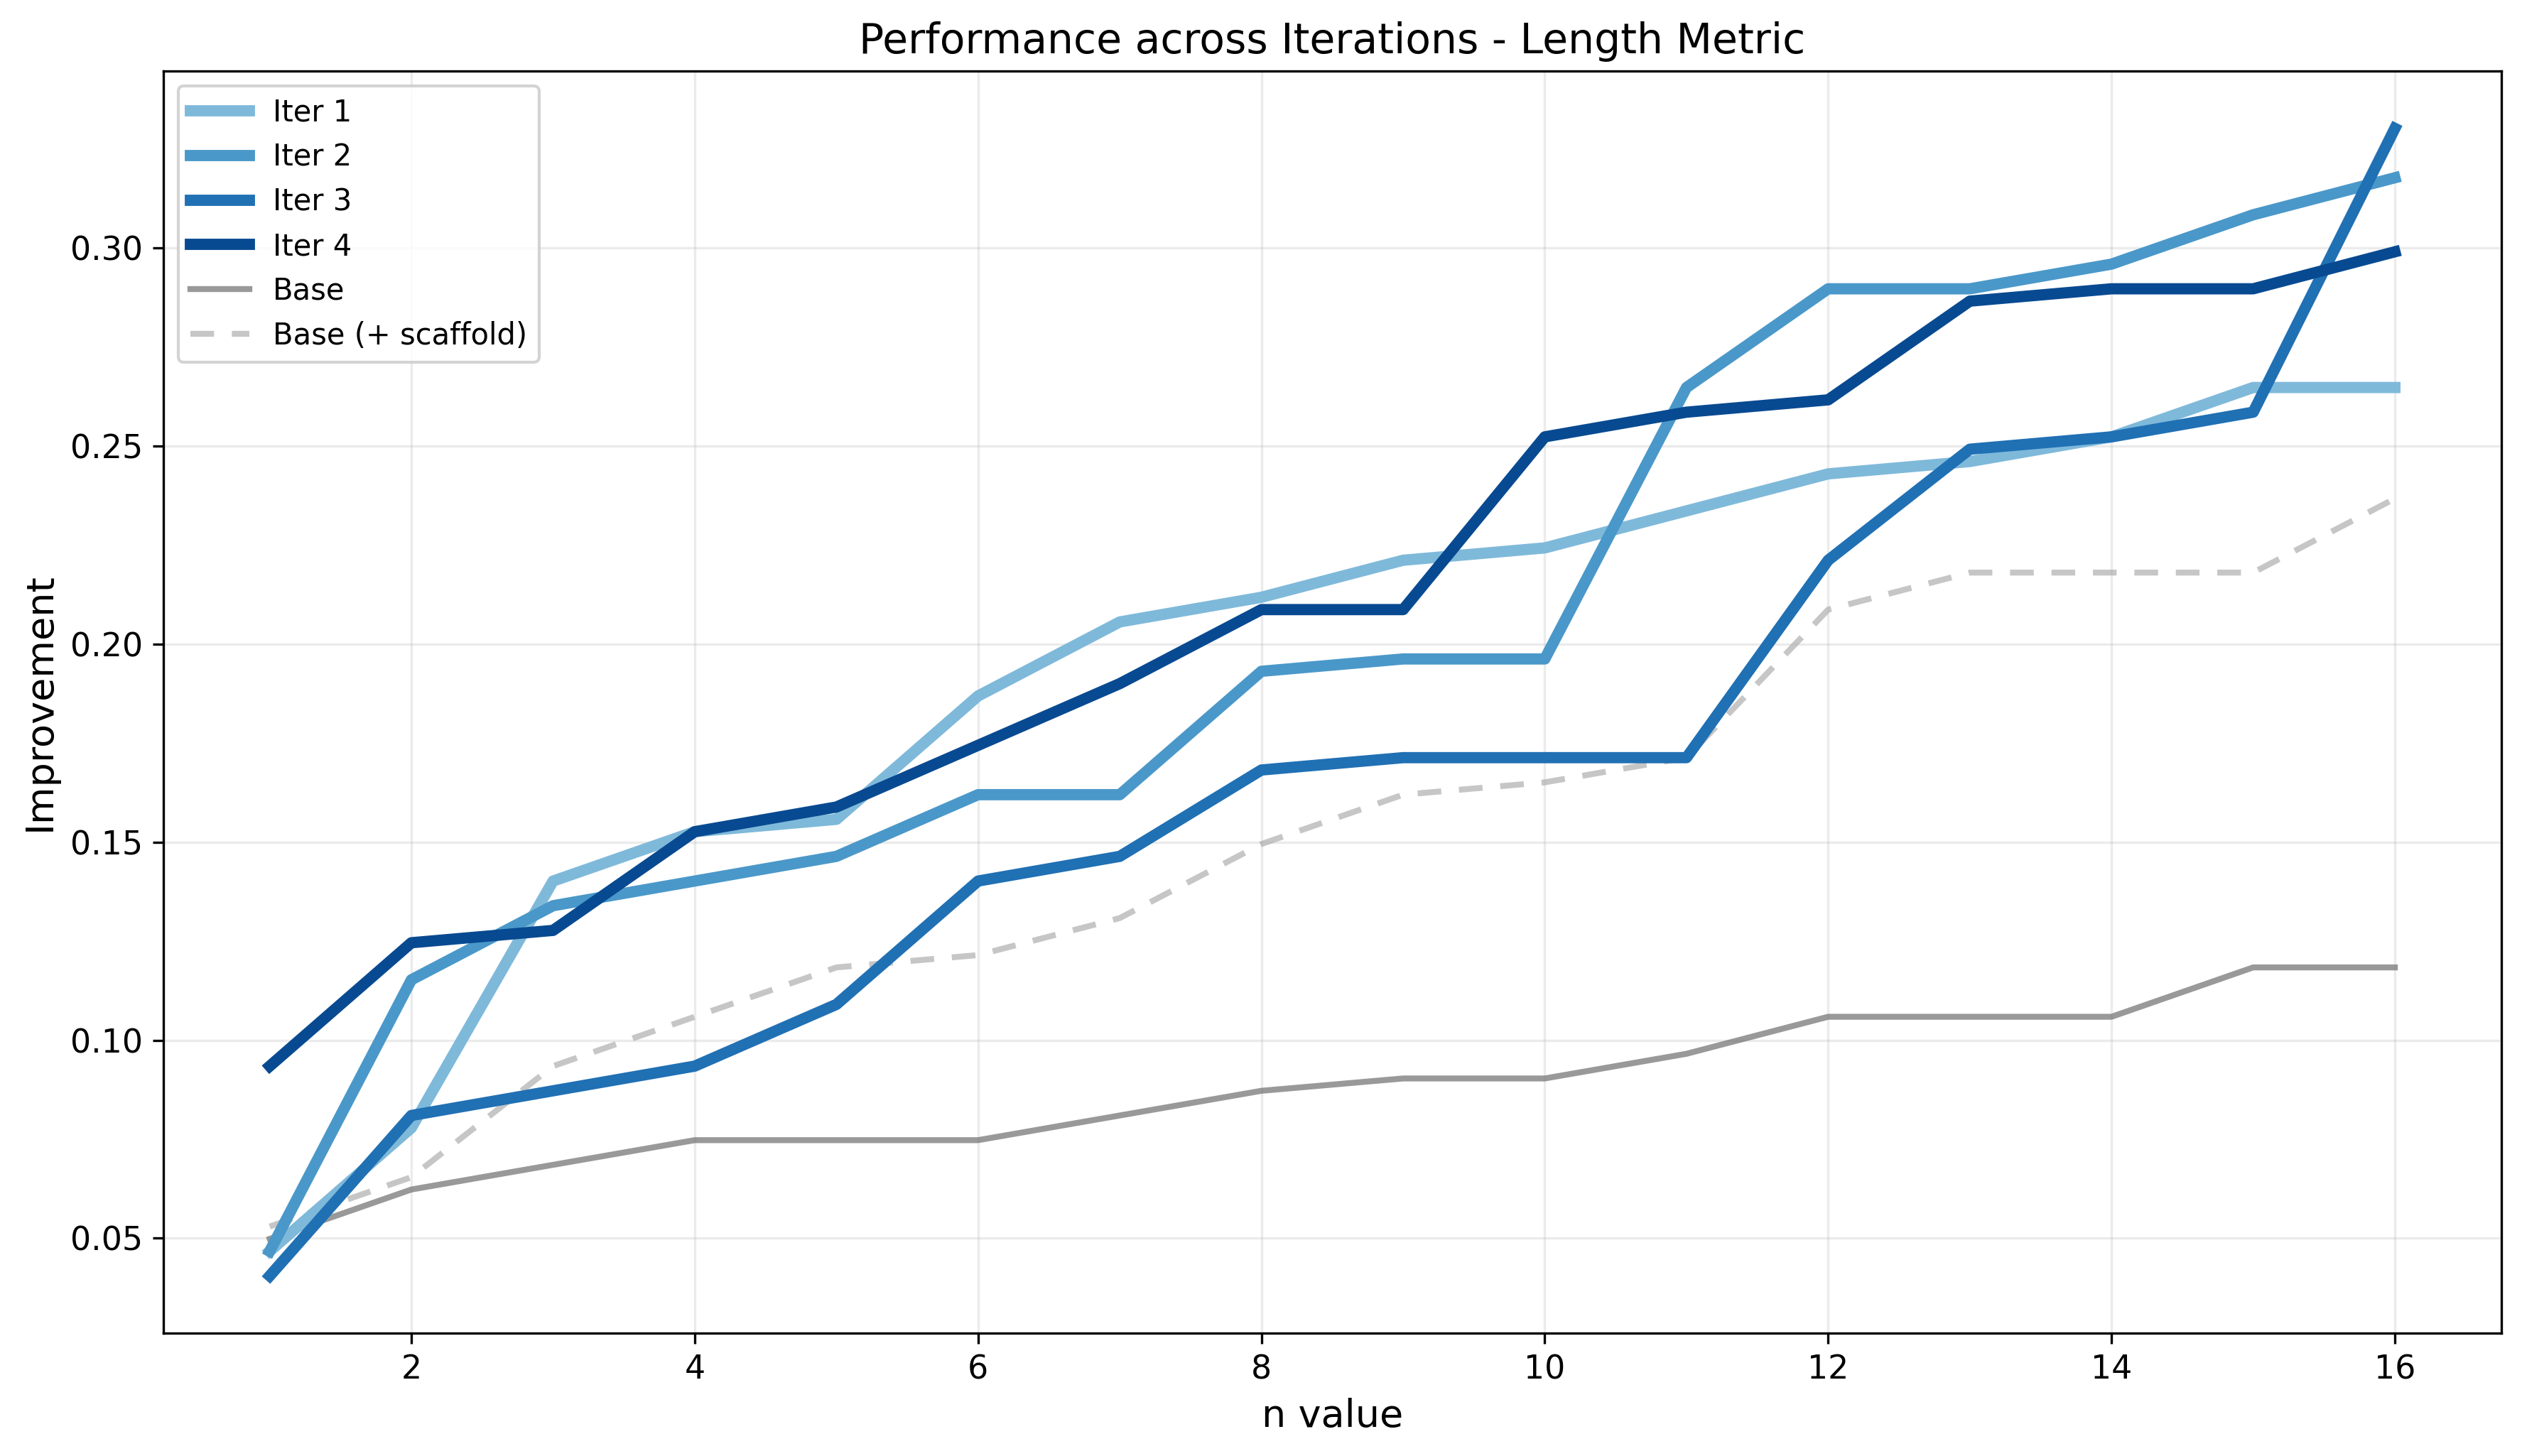
\includegraphics[width=\linewidth]{figures/Length/length_iterations.png}
\end{figure}
\end{column}
\end{columns}
\small Rapid gains in early rounds; saturation and mild regression after peak iteration on all three metrics.
\end{frame}

\begin{frame}{Per-Repository Heterogeneity}
\vspace{0.4em}
\begin{center}
\small
\begin{tabular}{l|ccc}
\toprule
\textbf{Repository} & \textbf{Length} & \textbf{Dep.} & \textbf{Mod.}\\
\midrule
HEPLean    & \good{1.283} & 0.379 & 0.030\\
ConNF      & 0.420 & 0.278 & 0.048\\
Seymour    & 0.199 & 0.100 & \good{0.359}\\
FLT        & 0.131 & 0.133 & 0.066\\
Foundation & 0.082 & 0.015 & 0.219\\
Carleson   & 0.048 & 0.188 & 0.095\\
Mathlib    & 0.016 & \good{0.306} & 0.163\\
\bottomrule
\end{tabular}
\end{center}
\end{frame}

\begin{frame}{Per-Repository Heterogeneity: Interpretation}
\vspace{0.8em}
\begin{itemize}\setlength{\itemsep}{12pt}
  \item \textbf{Mathlib}: proofs already concise (low length gain) but admit structural refactoring (high dep./mod.\ --- already well-optimized for length, still room for modularity)
  \item \textbf{HEPLean/ConNF}: large length/dependency gains --- proofs have more compression opportunity; less emphasis on existing automation
  \item \textbf{Seymour}: highest modularity gain ($0.359$) --- proof style admits natural decomposition into independent subgoals
  \item Results are descriptive; reflect stylistic differences and theorem difficulty distributions across repos
\end{itemize}
\end{frame}

\begin{frame}[fragile]{Qualitative: Dependency Reduction}
\vspace{0.2em}
{\small \texttt{isCoatom\_iff} (Mathlib.Order.Atoms) --- 5 named deps $\to$ 2}
\begin{columns}[T]
\begin{column}{0.50\textwidth}
\textbf{Original}
\begin{lstlisting}[basicstyle=\scriptsize\ttfamily]
theorem isCoatom_iff
    [OrderTop A] {K : A} :
    IsCoatom K $\leftrightarrow$
    K $\neq$ T $\wedge$ $\forall$ H g, K $\leq$ H
    $\to$ g $\notin$ K $\to$ g $\in$ H $\to$ H = T
    := by
  simp_rw [IsCoatom,
    lt_iff_le_not_le,
    SetLike.not_le_iff_exists,
    and_comm (a := _ $\leq$ _),
    and_imp, exists_imp,
    $\leftarrow$ and_imp, and_comm]
\end{lstlisting}
\end{column}
\begin{column}{0.47\textwidth}
\textbf{ImProver~2}
\begin{lstlisting}[basicstyle=\scriptsize\ttfamily]
theorem isCoatom_iff
    [OrderTop A] {K : A} :
    IsCoatom K $\leftrightarrow$
    K $\neq$ T $\wedge$ $\forall$ H g, K $\leq$ H
    $\to$ g $\notin$ K $\to$ g $\in$ H $\to$ H = T
    := by
  constructor <;> intro h
  <;> simp_all [IsCoatom,
    lt_iff_le_not_le,
    SetLike.not_le_iff_exists]
  <;> tauto
\end{lstlisting}
\vspace{0.3em}
\small Automation replaces brittle named-rewrite chain. 5 explicit deps $\to$ 2.
\end{column}
\end{columns}
\end{frame}

\begin{frame}[fragile]{Qualitative: Length Reduction (HEPLean)}
\vspace{0.2em}
{\small \texttt{summerCommute\_jacobi} (HEPLean.PerturbationTheory) --- 43 lines $\to$ 24 \good{($-$19 tactics)}}
\begin{columns}[T]
\begin{column}{0.54\textwidth}
\textbf{Original}
\begin{lstlisting}[basicstyle=\tiny\ttfamily]
lemma summerCommute_jacobi ... := by
  repeat rw [superCommuteF_ofCrAnListF_...]
  simp only [instCommGroup, map_sub, ...]
  repeat rw [superCommuteF_ofCrAnListF_...]
  simp only [instCommGroup.eq_1, ...]
  by_cases h1 : (FF |>s Phis1) = bosonic <;>
    by_cases h2 : (FF |>s Phis2) = bosonic <;>
    by_cases h3 : (FF |>s Phis3) = bosonic
  -- Case 1 of 8: all bosonic
  . simp only [h1, h2, h3,
      bosonic_exchangeSign, one_smul, ...]
    abel
  -- ... (6 more explicit simp/abel cases) ...
  . simp only [neq_bosonic_iff_eq_fermionic]
      at h1 h2 h3
    simp only [h1, h2, h3, mul_self, ...]
    abel
\end{lstlisting}
\end{column}
\begin{column}{0.42\textwidth}
\textbf{ImProver~2}
\begin{lstlisting}[basicstyle=\tiny\ttfamily]
lemma summerCommute_jacobi ... := by
  simp_all [
    superCommuteF_ofCrAnListF_...,
    instCommGroup, map_sub, map_smul,
    instCommGroup.eq_1,
    ofList_append_eq_mul,
    neq_bosonic_iff_eq_fermionic]
  <;> by_cases h1 : ... = bosonic
  <;> by_cases h2 : ... = bosonic
  <;> by_cases h3 : ... = bosonic
  <;> simp_all [h1, h2, h3,
      bosonic_exchangeSign,
      fermionic_exchangeSign_fermionic,
      bosonic_mul_fermionic, ...]
  <;> abel
\end{lstlisting}
\vspace{0.3em}
\small 8 explicit bosonic/fermionic case branches unified into single \texttt{simp\_all} + \texttt{abel} pass.
\end{column}
\end{columns}
\end{frame}

\begin{frame}[fragile]{Qualitative: Modularity Increase}
\vspace{0.2em}
{\small \texttt{KD\_weakerThan\_KDB} (Seymour) --- flat proof $\to$ 2 effective named subgoals}
\begin{columns}[T]
\begin{column}{0.40\textwidth}
\textbf{Original}
\begin{lstlisting}[basicstyle=\scriptsize\ttfamily,literate={<=s}{{$\leq_s$}}2]
lemma KD_weakerThan_KDB :
  (Hilbert.KD $\alpha$) <=s
  (Hilbert.KDB $\alpha$) :=
  normal_weakerThan_of_subset
    (by intro; aesop)
\end{lstlisting}
\small Flat; modularity $= 0$.
\end{column}
\begin{column}{0.57\textwidth}
\textbf{ImProver~2}
\begin{lstlisting}[basicstyle=\scriptsize\ttfamily,literate={<=s}{{$\leq_s$}}2 {subset}{{$\subseteq$}}1]
lemma KD_weakerThan_KDB :
  (Hilbert.KD $\alpha$) <=s
  (Hilbert.KDB $\alpha$) := by
  have h1 : KD.axioms subset
    KDB.axioms ->
    KD <=s KDB := by
    apply normal_weakerThan_of_subset
  have h2 : KD.axioms subset
    KDB.axioms := by
    intro phi hphi
    cases hphi <;>
      simp_all [KD, KDB]
  exact h1 h2
\end{lstlisting}
\small 2 effective spawned goals: $h_1$, $h_2$.
\end{column}
\end{columns}
\end{frame}

% ================================================================
\section{Conclusions}
% ================================================================

\begin{frame}{Summary: ImProver}
\vspace{0.5em}
\begin{itemize}\setlength{\itemsep}{8pt}
  \item \textbf{Task formalization}: proof optimization as a well-defined task with flexible metric framework; subsumes NTP as a strict special case
  \item \textbf{Chain-of-States}: mechanism for annotating intermediate proof states as generation context; single largest ablation contributor
  \item \textbf{Scaffold}: error correction, refinement loops, and RAG over Mathlib + TPiL
  \item \textbf{Results}: 423--778\% over GPT-4o baseline; 100\% compilation via fallback guarantee
  \item \textbf{Feasibility}: establishes that agentic prompting with frontier LLMs can produce meaningful proof optimization
\end{itemize}
\end{frame}

\begin{frame}{Summary: ImProver~2}
\vspace{0.3em}
\begin{itemize}\setlength{\itemsep}{5pt}
  \item \textbf{Training pipeline}: iterative self-improvement via IRPO; winner-winner pairs create dense reward signal beyond binary correctness
  \item \textbf{Replay buffer}: prevents model collapse; mixes historical and new data with improvement-rate filtering
  \item \textbf{Neurosymbolic scaffold}: context slice + CoS + auto-informalization consistently improves performance across all model sizes
  \item \textbf{New metrics}: modularity and dependencies with kernel-level reward-hacking guards
  \item \textbf{Results}: 7B model outperforms 671B on all structural metrics; competitive with frontier on dependencies; leads all on modularity
\end{itemize}
\end{frame}

\begin{frame}{Limitations: ImProver}
\vspace{0.8em}
\begin{enumerate}\setlength{\itemsep}{12pt}
  \item[\bad{1.}] \textbf{Cost}: many GPT-4o API calls + document retrieval per theorem; library-scale deployment infeasible at current pricing
  \item[\bad{2.}] \textbf{Closed-source}: tightly coupled to GPT-4o; non-reproducible; subject to model deprecation
  \item[\bad{3.}] \textbf{Small evaluation}: only $72 + 26 + 43 = 141$ theorems; toy datasets not representative of real research repositories with inter-file dependencies
  \item[\bad{4.}] \textbf{Weak metrics}: declarativity gameable via \texttt{have}-padding; no kernel-level structural metric
\end{enumerate}
\end{frame}

\begin{frame}{Limitations: ImProver~2}
\vspace{0.8em}
\begin{enumerate}\setlength{\itemsep}{12pt}
  \item[\bad{1.}] \textbf{Unvalidated metrics}: structural metrics (modularity, dependencies) not validated against human-maintainer preferences via a formal study
  \item[\bad{2.}] \textbf{Single-step generator}: no recovery when rewrite fails --- deliberate design choice to study training dynamics before adding agentic complexity
  \item[\bad{3.}] \textbf{Training saturation}: saturates after 2--4 rounds on fixed dataset; escaping saturation requires larger preference datasets or explicit curriculum growth
\end{enumerate}
\end{frame}

\begin{frame}{Future Work: Near-Term}
\vspace{0.8em}
\begin{enumerate}\setlength{\itemsep}{12pt}
  \item \textbf{Trained iterative revision}\\
    \small Internalize ImProver's error-correction loop into model weights; train the model to know when to stop, when to revise, and how to incorporate compiler feedback
  \item \textbf{Human preference study}\\
    \small Validate modularity/dependency metrics against formal mathematician judgments via a controlled, blinded study
  \item \textbf{Richer metrics}\\
    \small LLM-as-judge readability scoring; robustness to library version updates; maintainability proxies
\end{enumerate}
\end{frame}

\begin{frame}{Future Work: Longer-Term}
\vspace{0.8em}
\begin{enumerate}\setlength{\itemsep}{12pt}
  \item \textbf{Library-level optimization}\\
    \small Maintain consistency across inter-dependent Mathlib rewrites; ensure a modular refactor of one theorem does not break downstream proofs referencing its intermediate names
  \item \textbf{Close the training data loop}\\
    \small Empirically show that provers trained on ImProver/ImProver~2-optimized corpora outperform those trained on unoptimized data --- confirming the data quality hypothesis
  \item \textbf{Autoformalization quality}\\
    \small Use proof optimization to make machine-formalized proofs (e.g.\ AlphaProof outputs) human-readable and maintainable
\end{enumerate}
\end{frame}

\begin{frame}{Closing Remarks}
\vspace{0.2em}
\begin{itemize}\setlength{\itemsep}{4pt}
  \item Formal libraries are growing faster than human maintainers can curate them
  \item AI-generated proofs will flood these libraries --- automated quality improvement is necessary
  \item \textbf{Central insight}: giving a model access to formal proof structure --- via CoS at inference time, via neurosymbolic augmentation at training time --- enables far more substantive proof transformations
  \item Proof optimization is feasible, learnable, and applies to both library maintenance and training data quality
\end{itemize}
\vspace{0.2em}
\begin{exampleblock}{}
  \centering\small ImProver and ImProver~2 establish proof optimization as a foundation for AI-assisted formal mathematics.
\end{exampleblock}
\end{frame}

\begin{frame}[standout]
\centering
\Large Thank you!\\[0.8em]
\normalsize
\textbf{ImProver}: ICLR 2025\\[0.3em]
\textbf{ImProver~2}: ICML 2026 (submitted)\\[0.8em]
\small Questions welcome.
\end{frame}

\end{document}
